%% LyX 2.0.6 created this file.  For more info, see http://www.lyx.org/.
%% Do not edit unless you really know what you are doing.
\documentclass[english]{beamer}
\usepackage{mathptmx}
\renewcommand{\sfdefault}{lmss}
\usepackage[T1]{fontenc}
\usepackage[latin9]{inputenc}
\usepackage{array}
\usepackage{calc}
\usepackage{multirow}
\usepackage{amsmath}
\usepackage{amssymb}
\usepackage{graphicx}

\makeatletter

%%%%%%%%%%%%%%%%%%%%%%%%%%%%%% LyX specific LaTeX commands.
%% Because html converters don't know tabularnewline
\providecommand{\tabularnewline}{\\}

%%%%%%%%%%%%%%%%%%%%%%%%%%%%%% Textclass specific LaTeX commands.
 % this default might be overridden by plain title style
 \newcommand\makebeamertitle{\frame{\maketitle}}%
 \AtBeginDocument{
   \let\origtableofcontents=\tableofcontents
   \def\tableofcontents{\@ifnextchar[{\origtableofcontents}{\gobbletableofcontents}}
   \def\gobbletableofcontents#1{\origtableofcontents}
 }
 \long\def\lyxframe#1{\@lyxframe#1\@lyxframestop}%
 \def\@lyxframe{\@ifnextchar<{\@@lyxframe}{\@@lyxframe<*>}}%
 \def\@@lyxframe<#1>{\@ifnextchar[{\@@@lyxframe<#1>}{\@@@lyxframe<#1>[]}}
 \def\@@@lyxframe<#1>[{\@ifnextchar<{\@@@@@lyxframe<#1>[}{\@@@@lyxframe<#1>[<*>][}}
 \def\@@@@@lyxframe<#1>[#2]{\@ifnextchar[{\@@@@lyxframe<#1>[#2]}{\@@@@lyxframe<#1>[#2][]}}
 \long\def\@@@@lyxframe<#1>[#2][#3]#4\@lyxframestop#5\lyxframeend{%
   \frame<#1>[#2][#3]{\frametitle{#4}#5}}
 \def\lyxframeend{} % In case there is a superfluous frame end

%%%%%%%%%%%%%%%%%%%%%%%%%%%%%% User specified LaTeX commands.
%\usetheme{Warsaw}
%\usetheme{Boadilla}
%\usetheme{Madrid}
\usetheme{Frankfurt}
\usepackage{tikz}
\usetikzlibrary{decorations.pathreplacing} 

\setbeamertemplate{itemize subitem}{\tiny\raise1.5pt\hbox{\donotcoloroutermaths$\blacktriangleright$}}
\setbeamertemplate{itemize subsubitem}{\tiny\raise1.5pt\hbox{\donotcoloroutermaths$-$}}

\setbeamersize{text margin left=0.3cm,text margin right=0.5cm}
\usecolortheme{orchid}
\setbeamertemplate{footline}[text line]
{
 \leavevmode%
    \hspace*{0.9\paperwidth}
    \insertframenumber{} / \inserttotalframenumber%\hspace*{1ex}
}

\setbeamertemplate{navigation symbols}{}

\setbeamercovered{transparent}
% or whatever (possibly just delete it)

\makeatother

\usepackage{babel}
\begin{document}

\title{Limit determination - Emphasis on arbitrariness}


\author{E. Busato}

\makebeamertitle

\lyxframeend{}\lyxframe{Outline}

\tableofcontents{}


\lyxframeend{}\section{Introduction}


\lyxframeend{}\lyxframe{Standard cut\&count problem}
\begin{block}
<1->{Notations}
\begin{itemize}
\item One or more backgrounds: \textcolor{blue}{$\sum b_{i}$}
\item Signal with unknown x-sec: \textcolor{blue}{$s$} (free parameter)
\item Total expectation: \textcolor{blue}{$s+\sum b_{i}$}
\item Observed number of events: \textcolor{blue}{$N_{\text{obs}}$}
\end{itemize}
\end{block}

\pause{}
\begin{itemize}
\item When $N_{\text{obs}}$ agrees with background yield, infer upper limit
$s_{\text{up}}$


\begin{center}


\textcolor{red}{$\boxed{s_{\text{up}}=\text{yield above which total expectation and observation disagree}}$}


\end{center}

\end{itemize}

\pause{}
\begin{itemize}
\item \textcolor{blue}{To set limit one needs to}

\begin{itemize}
\item \textcolor{blue}{Know how $N_{\text{obs}}$ is distributed\vspace*{0.1cm}}
\item \textcolor{blue}{Have a quantitative measure of the agreement between
data and total expectation}
\end{itemize}
\end{itemize}

\lyxframeend{}\lyxframe{Distribution of $N_{\text{obs}}$ - Terminology}
\begin{itemize}
\item Distribution of observation described by \textcolor{red}{likelihood}
${\cal L}$:


\begin{center}


${\cal L}=\text{proba}(N_{\text{obs}};s+\sum\limits _{i}b_{i})$


\end{center}

\item Likelihood also called \textcolor{red}{statistical model} or \textcolor{red}{model}
\end{itemize}

\lyxframeend{}\lyxframe{Two central problems to be addressed}
\begin{enumerate}
\item \textcolor{blue}{Build statistical model}
\item \textcolor{blue}{Infer $s_{\text{up}}$ from statistical model (i.e.
quantify agreement between observation and total expectation for each
$s$)}
\end{enumerate}

\pause{}

\vspace*{1cm}

Important point: \textcolor{red}{no unique solution to these problems}

\vspace*{0.5cm}

$\rightarrow$ upper limit is a somewhat subjective notion (always
relative to the choices made to solve these problems)


\lyxframeend{}\lyxframe{Softwares}
\begin{itemize}
\item Throughout the presentation, three softwares implementing solutions
to previous problems will be discussed/compared/studied

\begin{itemize}
\item \textcolor{red}{McLimit}: hybrid frequentist-bayesian\textcolor{blue}{\vspace*{0.1cm}}
\item \textcolor{red}{CLsGenerator}: hybrid frequentist-bayesian\textcolor{blue}{\vspace*{0.1cm}}
\item \textcolor{red}{BayesianMCMC}: bayesian (Markov Chain Monte Carlo)
\end{itemize}
\end{itemize}
\textcolor{blue}{\vspace*{0.1cm}}
\begin{itemize}
\item HistFactory and various RooStats implementations (almost) not described
\end{itemize}

\lyxframeend{}\lyxframe{CLsGenerator and BayesianMCMC}
\begin{itemize}
\item Use exactly the same statistical model

\begin{itemize}
\item Difference is on how inference is made
\end{itemize}
\end{itemize}
\textcolor{blue}{\vspace*{0.2cm}}
\begin{itemize}
\item Take same files as input

\begin{itemize}
\item Comparison straightforward
\end{itemize}
\end{itemize}

\lyxframeend{}\section{Single channel - No uncertainties}


\lyxframeend{}\lyxframe{}

\begin{center}
\vspace*{2cm}
{\Large Single channel - No uncertainties}
\end{center}


\lyxframeend{}\lyxframe{Statistical model and inference}
\begin{enumerate}
\item \textbf{Statistical model}


In our experiments, $N_{\text{obs}}\sim Binomial$%
\footnote{$\sim$ means ``is distributed according to''%
}$\rightarrow$ Approximated by Poisson


\begin{center}


$\boxed{{\cal L}=\frac{\left(s+\sum\limits _{i}b_{i}\right)^{N_{\text{obs}}}}{N_{\text{obs}}!}e^{-\left(s+\sum\limits _{i}b_{i}\right)}}$


\end{center}


\pause{}

\item \textbf{Inference of $s_{\text{up}}$ }

\begin{itemize}
\item Two families of methods: \textcolor{red}{frequentist} and \textcolor{red}{bayesian}
\end{itemize}
\end{enumerate}

\lyxframeend{}\lyxframe{Frequentist solution}
\begin{itemize}
\item Consider the case: $N_{\text{obs}}=1$ and $\sum\limits _{i}b_{i}=0.82$
\end{itemize}
\begin{figure}
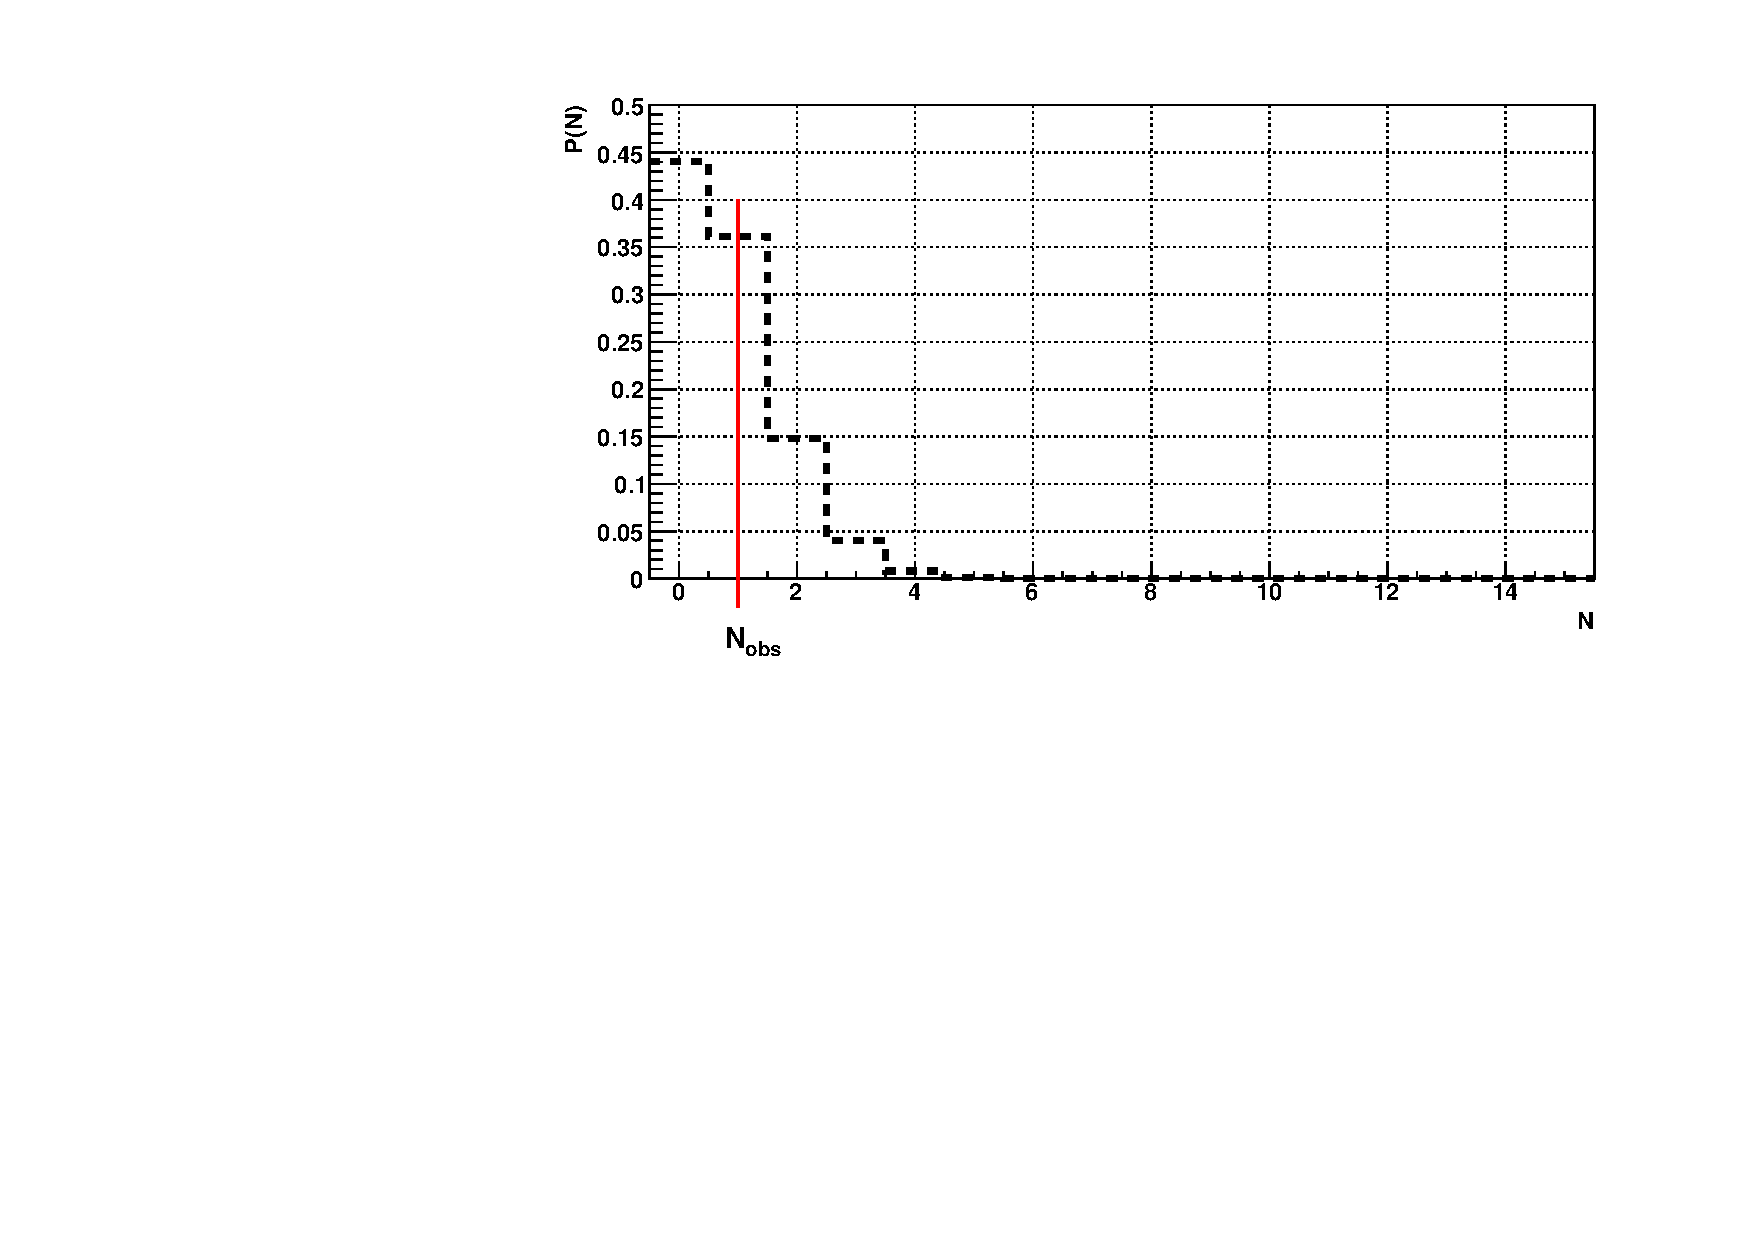
\includegraphics[scale=0.5]{macros/poissonDistributionBkgOnly}

\end{figure}



\lyxframeend{}\lyxframe{Frequentist solution}
\begin{itemize}
\item Consider the case: $N_{\text{obs}}=1$ and $\sum\limits _{i}b_{i}=0.82$
\end{itemize}
\begin{figure}
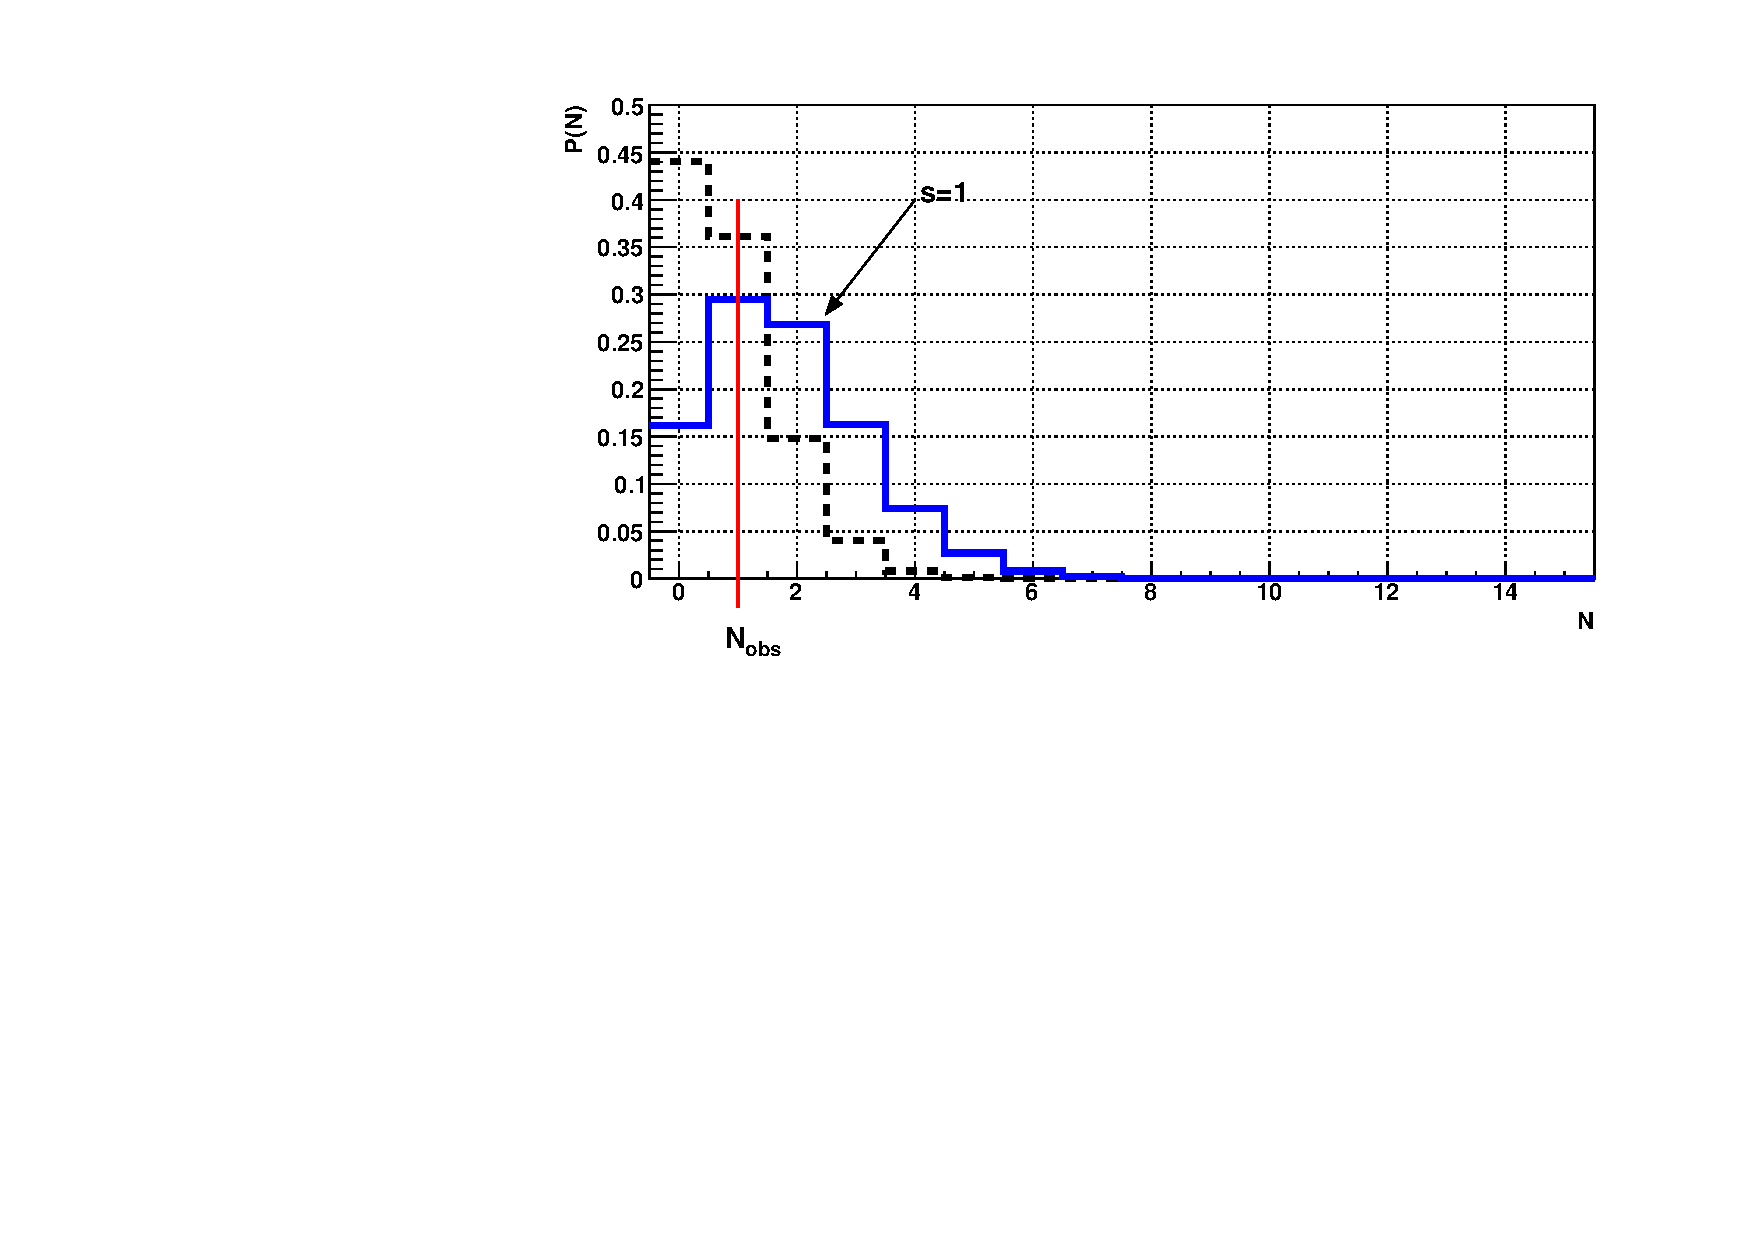
\includegraphics[scale=0.5]{macros/poissonDistributionSig1}
\end{figure}



\lyxframeend{}\lyxframe{Frequentist solution}
\begin{itemize}
\item Consider the case: $N_{\text{obs}}=1$ and $\sum\limits _{i}b_{i}=0.82$
\end{itemize}
\begin{figure}
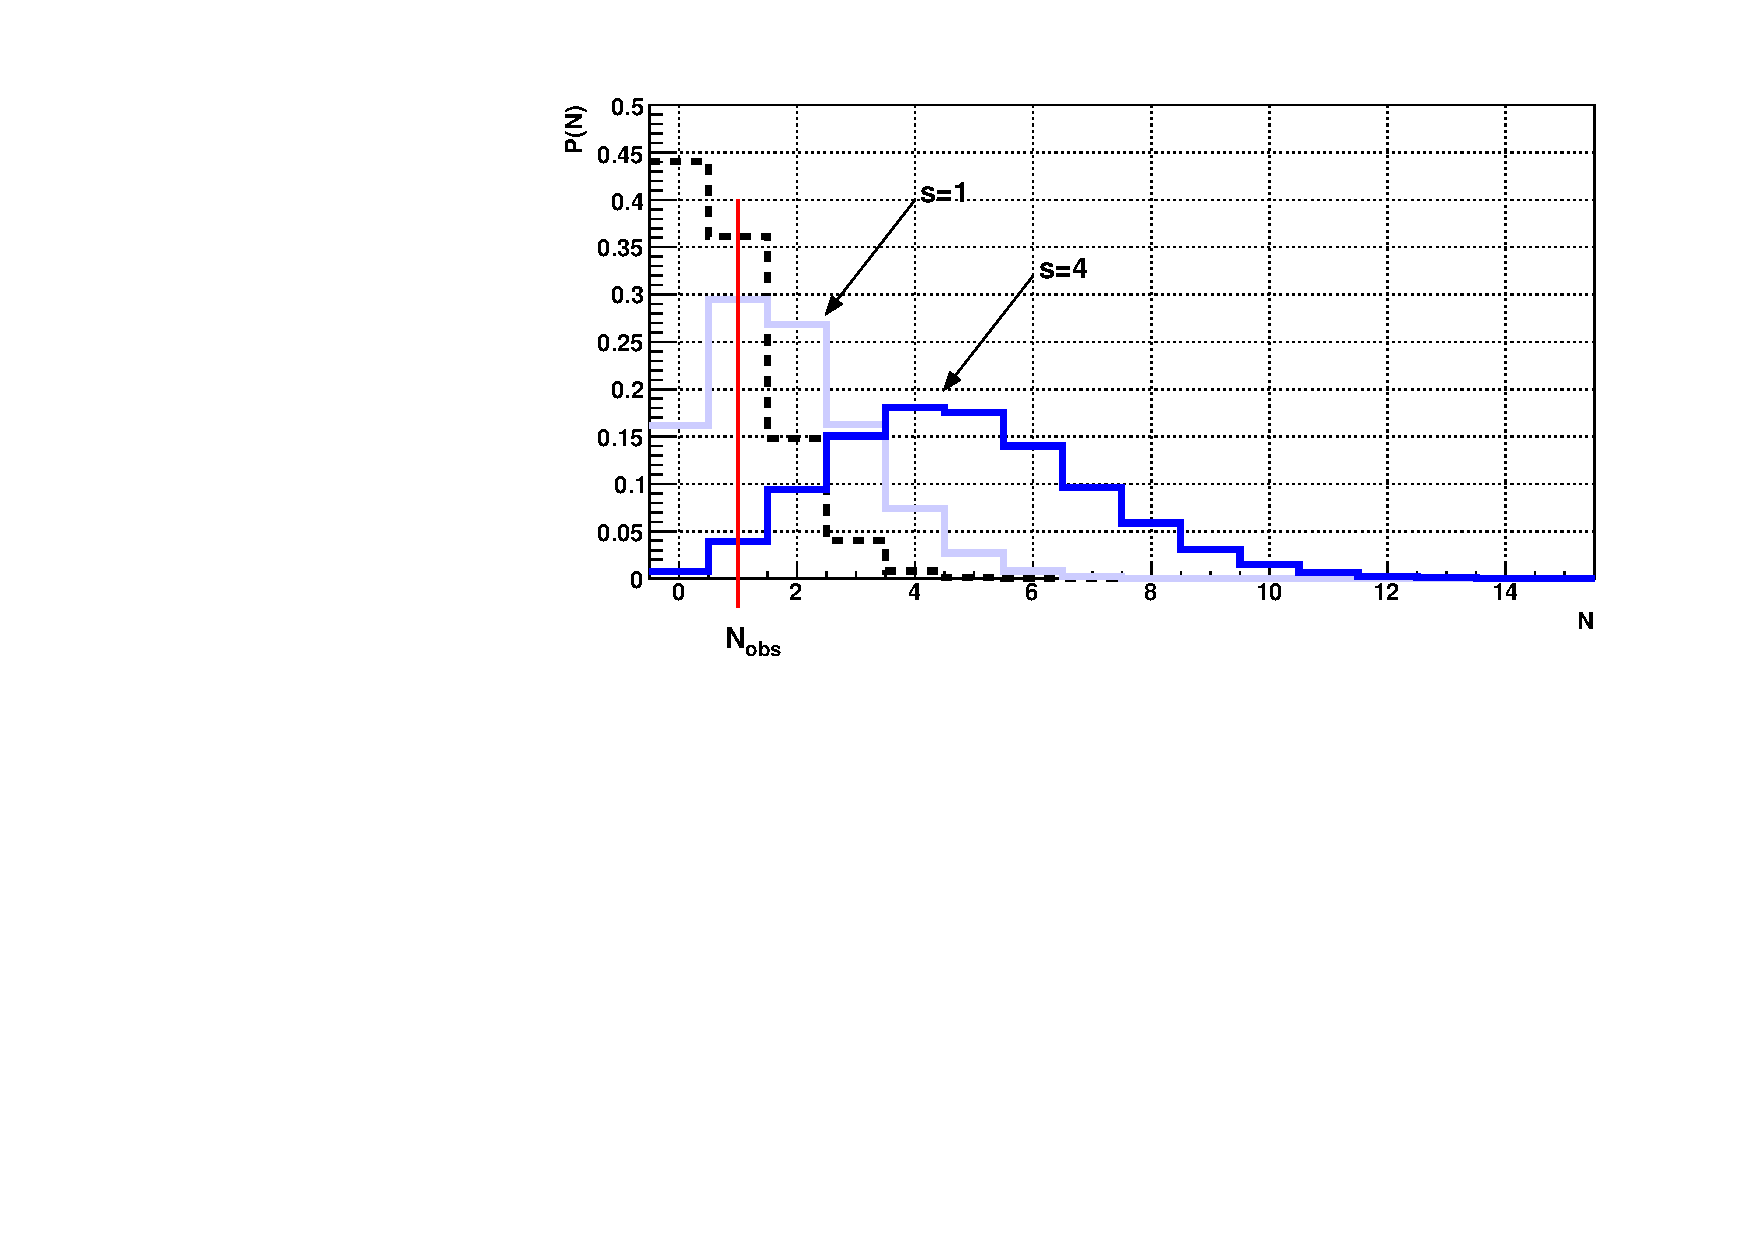
\includegraphics[scale=0.5]{macros/poissonDistributionSig4}
\end{figure}



\lyxframeend{}\lyxframe{Frequentist solution}
\begin{itemize}
\item Consider the case: $N_{\text{obs}}=1$ and $\sum\limits _{i}b_{i}=0.82$
\end{itemize}
\begin{figure}
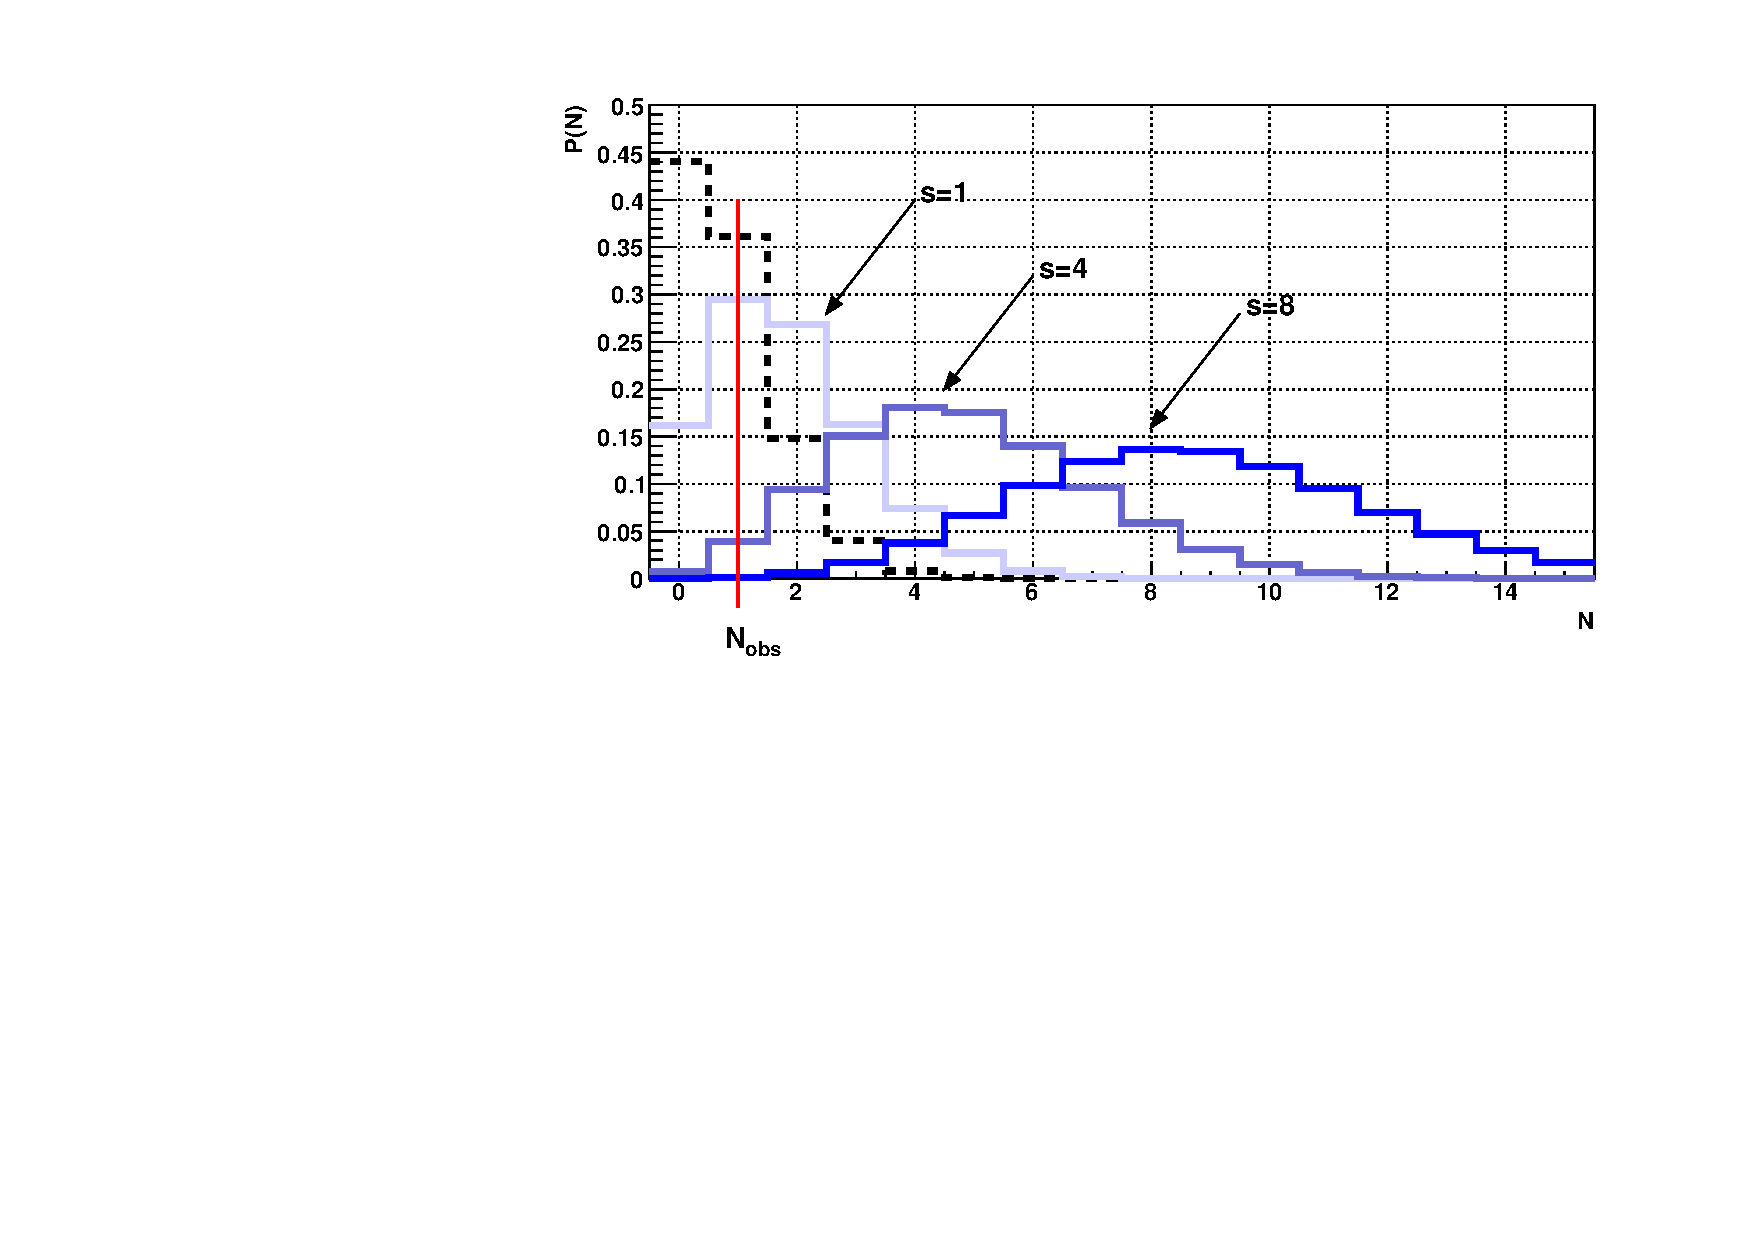
\includegraphics[scale=0.5]{macros/poissonDistributionSig8}
\end{figure}



\lyxframeend{}\lyxframe{Frequentist solution - $CL_{s+b}$ method}
\begin{itemize}
\item Quantitative measure of agreement: $p-value$


\begin{center}


$p-value=\underbrace{\sum\limits _{N=0}^{N_{\text{obs}}}{\cal P}(N;s+\sum\limits _{i}b_{i})}_{\text{c. d. f. }}=\sum\limits _{N=0}^{N_{\text{obs}}}\frac{\left(s+\sum\limits _{i}b_{i}\right)^{N}}{N!}e^{-\left(s+\sum\limits _{i}b_{i}\right)}$


\end{center}

\end{itemize}
\begin{figure}
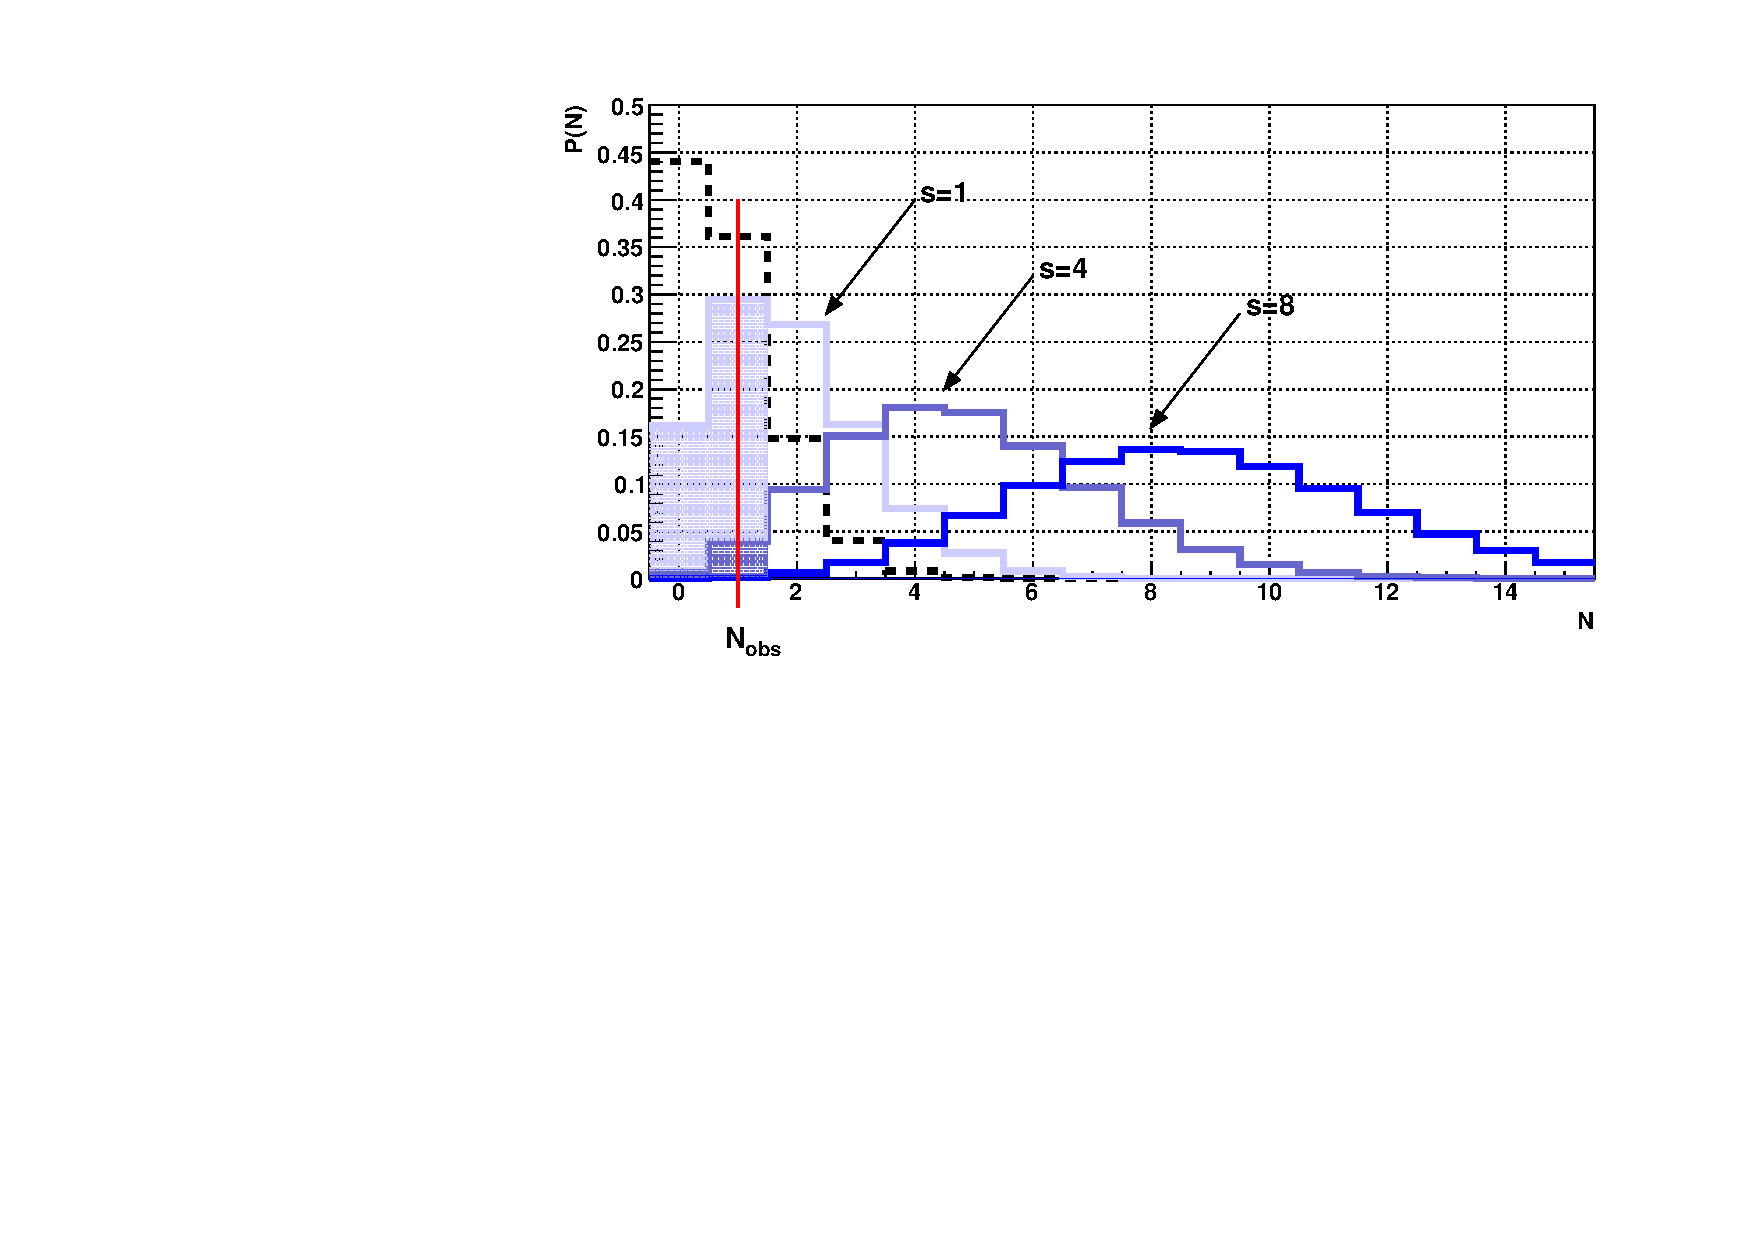
\includegraphics[scale=0.4]{macros/poissonDistributionSig8Pval}
\end{figure}


\vspace*{-0.2cm}
\begin{itemize}
\item \textcolor{magenta}{Remark: this $p-value$ is also called $CL_{s+b}$}
\end{itemize}

\lyxframeend{}\lyxframe{Frequentist solution - $CL_{s+b}$ method}
\begin{itemize}
\item For which values of $s$ does the observation disagree with total
expectation ?

\begin{itemize}
\item Usually we take values for which $p-value\leq\alpha$ with $\alpha=0.05$
\end{itemize}
\end{itemize}

\pause{}
\begin{itemize}
\item Upper limit $s_{\text{up}}$ is the smallest of all values for which
observation and total expectation disagree


\begin{center}


$\boxed{CL_{s+b}(s_{\text{up}})=\alpha}$


\end{center}

\end{itemize}

\pause{}
\begin{itemize}
\item Previous example: $s_{\text{up}}=3.92$
\end{itemize}

\lyxframeend{}\lyxframe{Frequentist solution - $CL_{s+b}$ method}

\begin{figure}
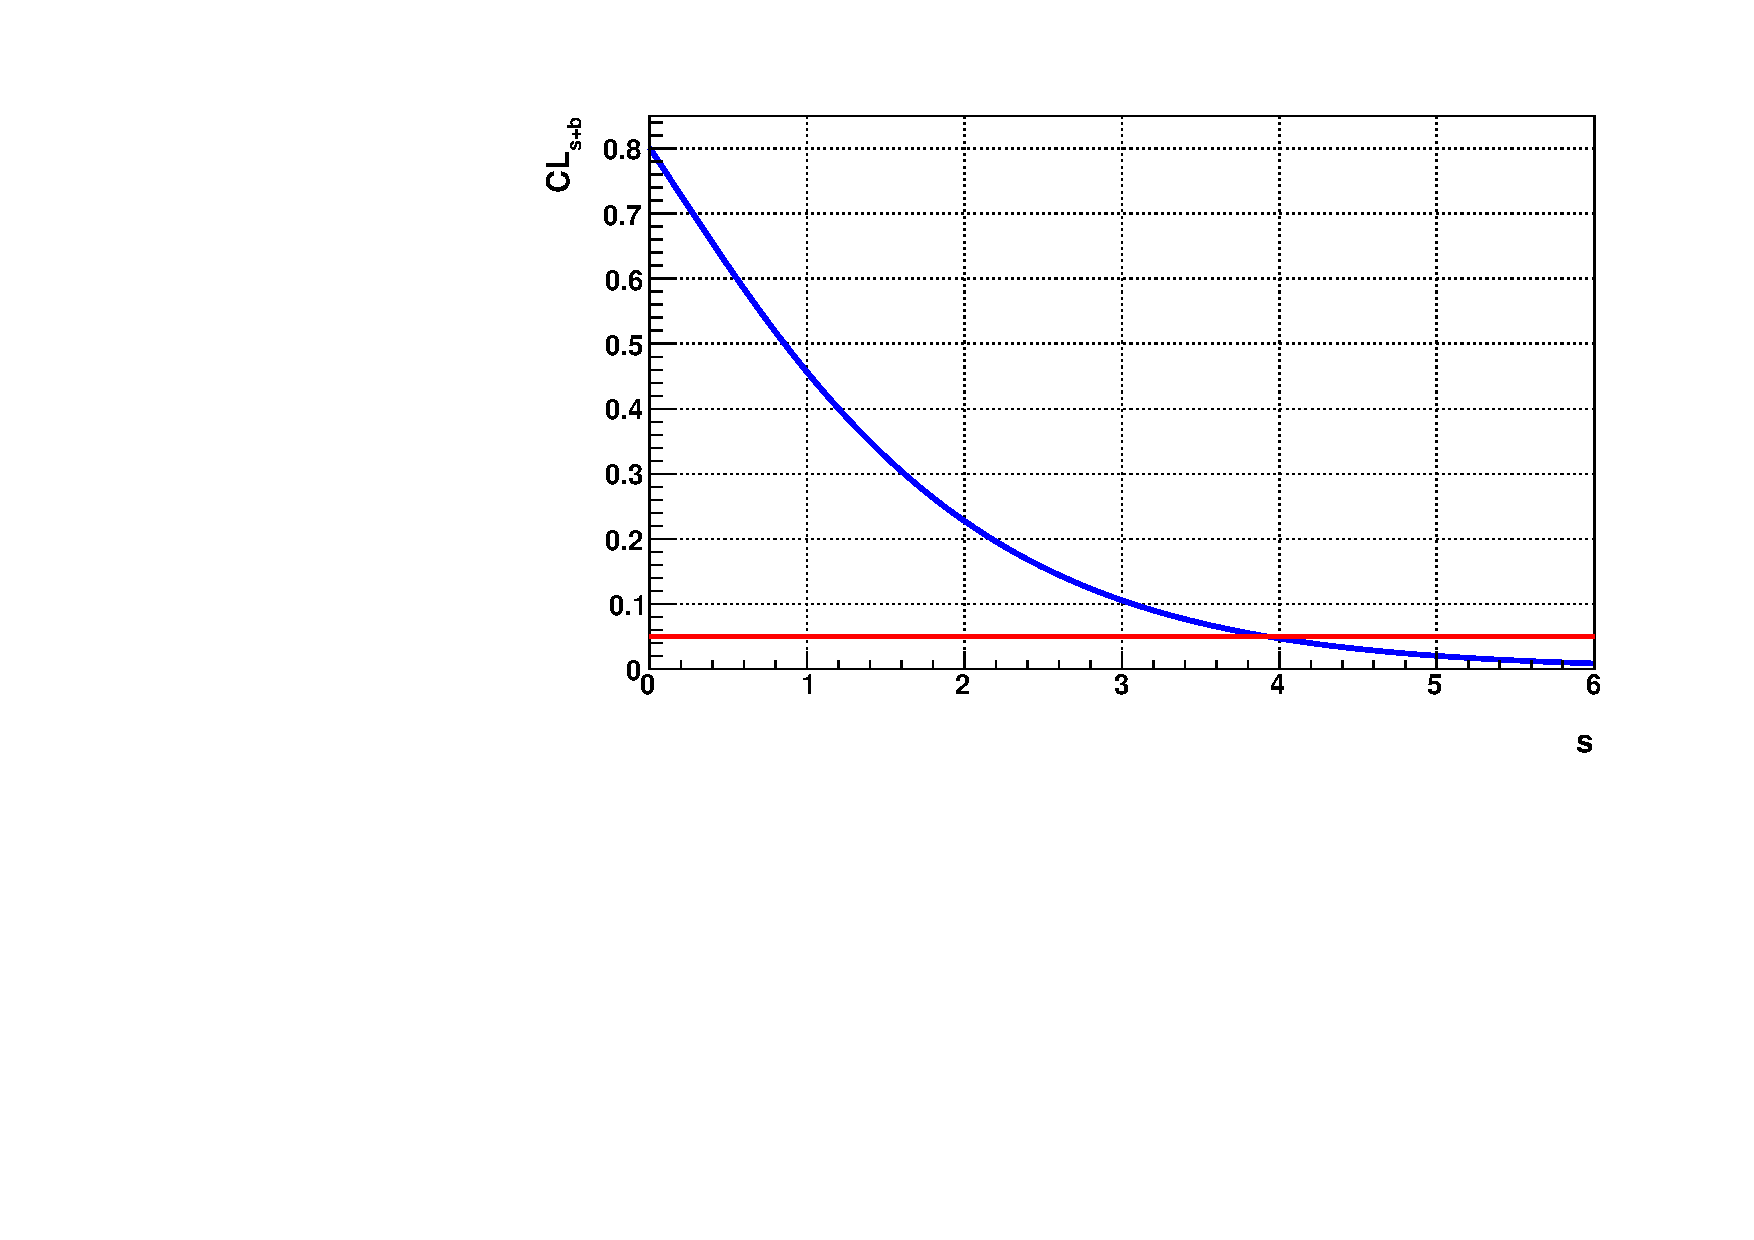
\includegraphics[scale=0.5]{macros/plotCLsbVsS_1}
\end{figure}



\lyxframeend{}\lyxframe{Frequentist solution - $CL_{s+b}$ method}
\begin{itemize}
\item Even though $CL_{s+b}$ seems a valid method, it's has a problem
\end{itemize}
\begin{figure}
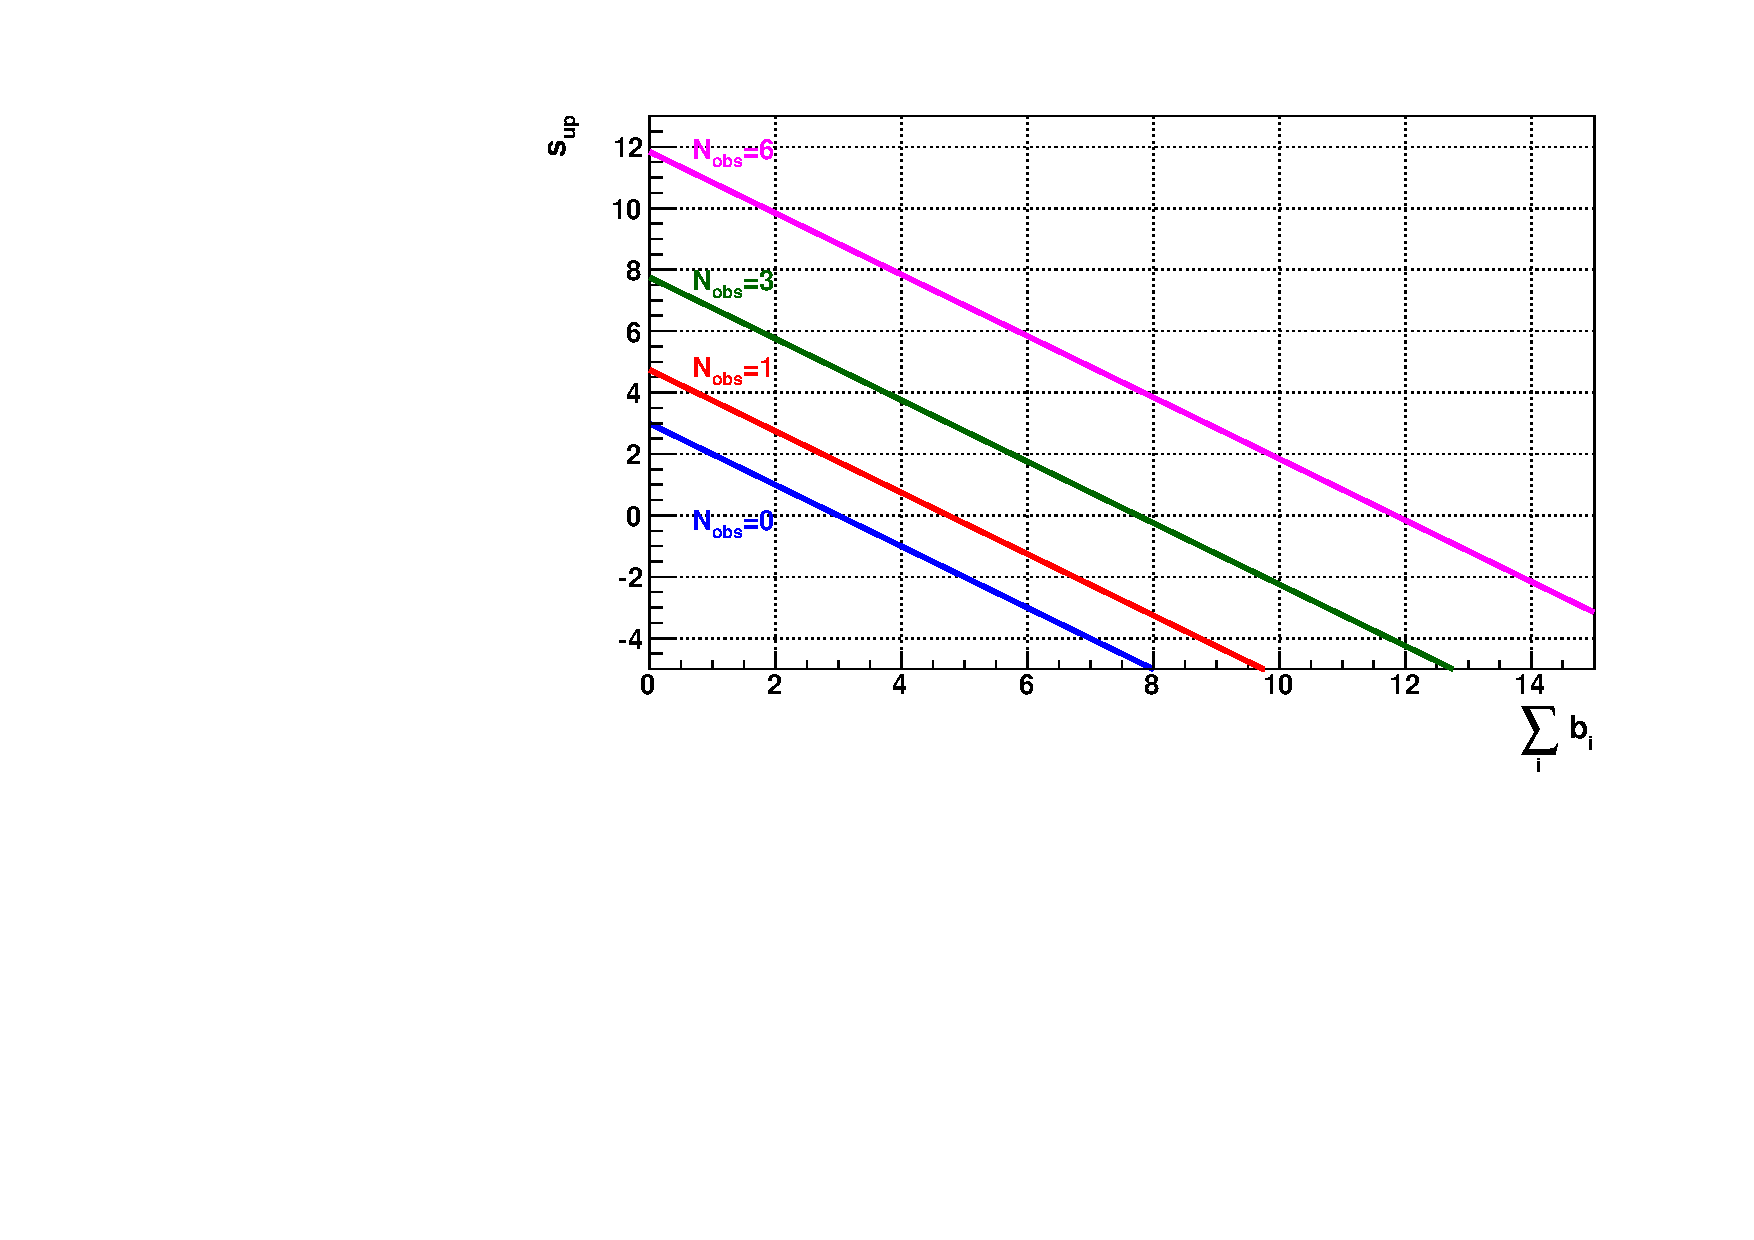
\includegraphics[scale=0.35]{macros/plotLimitVsNbkg_CLsb_1}
\end{figure}


\begin{center}$\rightarrow$ downward fluctuation leads to $s_{\text{up}}<\text{0}$
! \end{center}


\pause{}
\begin{itemize}
\item A fix could be to impose $s_{\text{up }}\geq0$ 


$\rightarrow$ Not satisfactory: all models predicting signal (even
those predicting very small yield) are excluded with 5\% probability

\end{itemize}

\lyxframeend{}\lyxframe{Frequentist solution - $CL_{s}$ method}
\begin{itemize}
\item Solution to previous issue: $CL_{s}$
\item Instead of defining $s_{\text{up}}$ by $CL_{s+b}(s_{\text{up}})=\alpha$,
define it by


\begin{center}


$\boxed{CL_{s}(s_{\text{up}})=\alpha}$


\end{center}


where $CL_{s}=\frac{CL_{s+b}}{CL_{b}}$, with


\begin{center}


$CL_{b}=\sum\limits _{N=0}^{N_{\text{obs}}}\frac{\left(\sum b_{i}\right)^{N}}{N!}e^{-\sum b_{i}}$


\end{center}

\end{itemize}

\lyxframeend{}\lyxframe{Frequentist solution - $CL_{s}$ method}

\begin{figure}
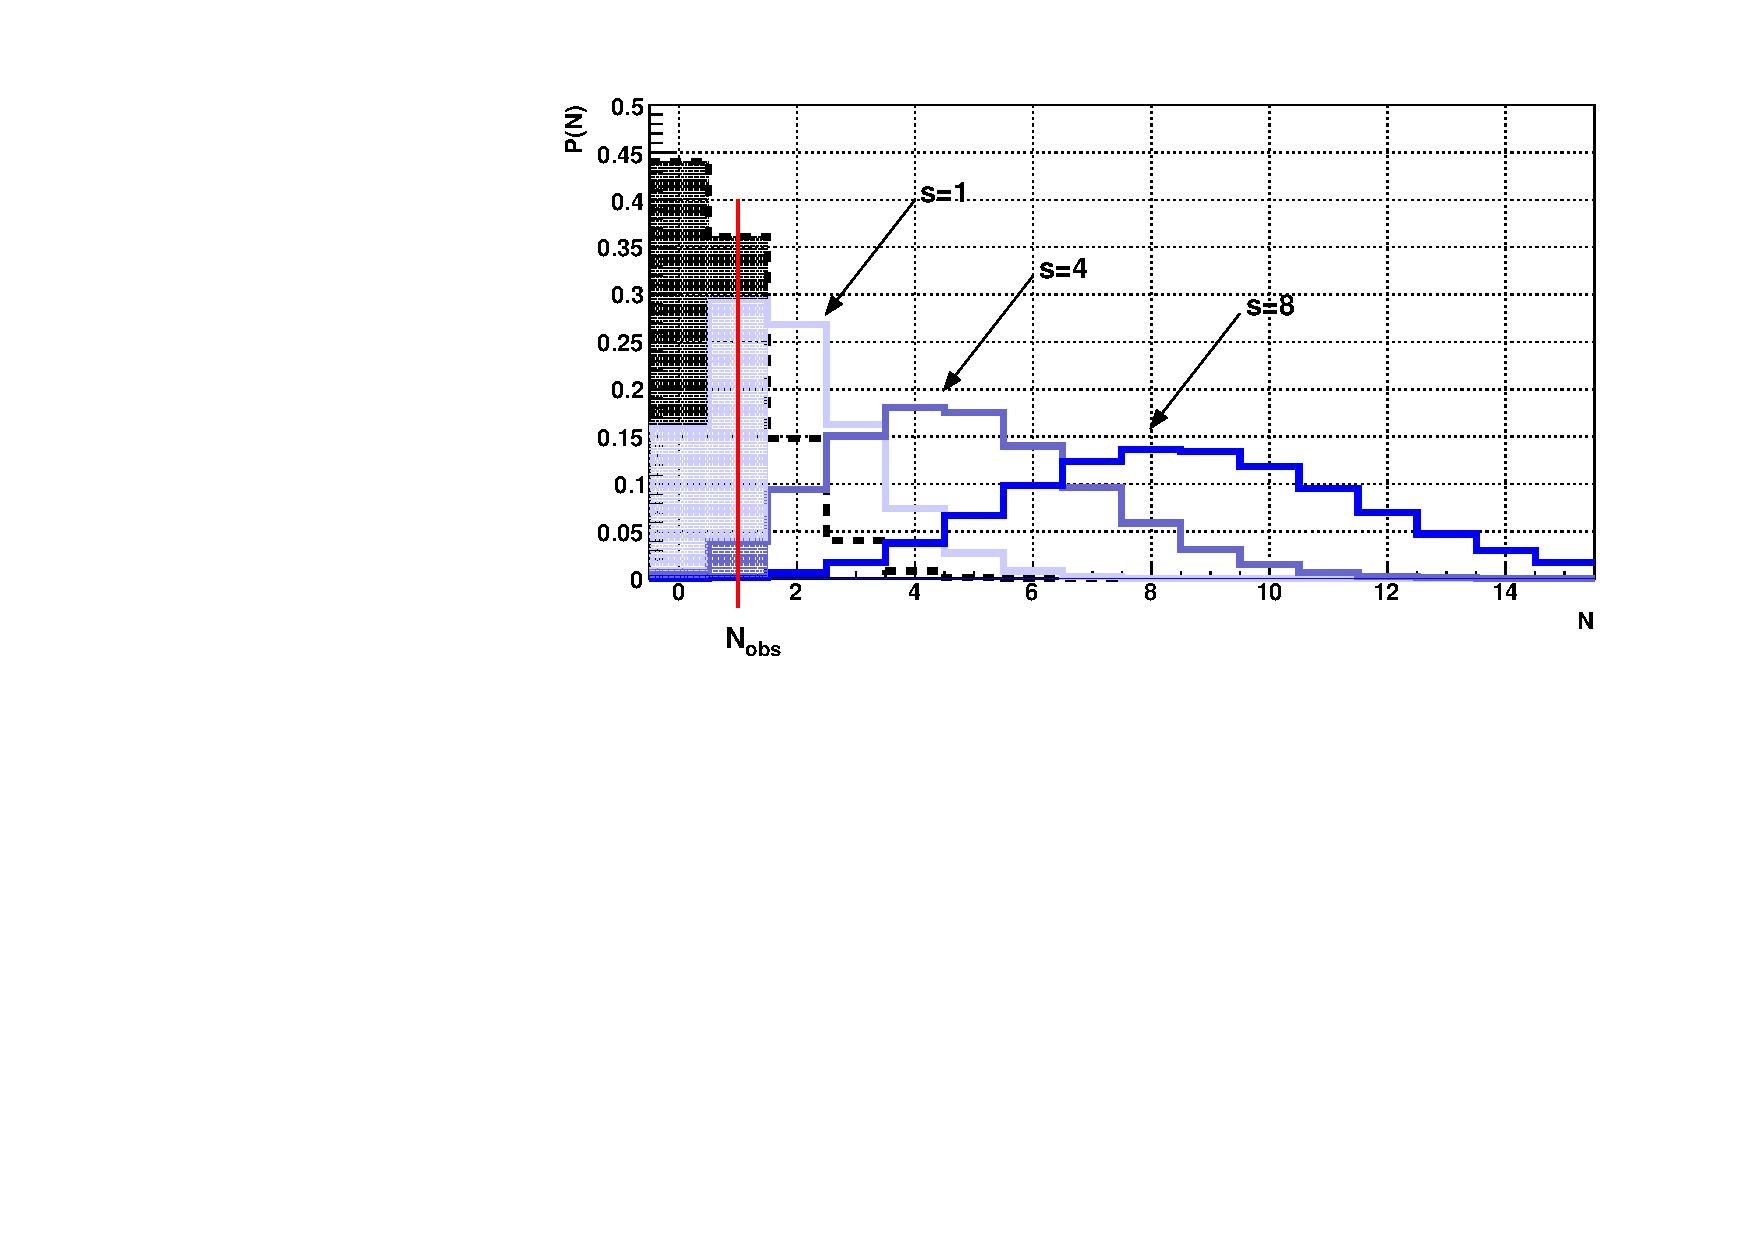
\includegraphics[scale=0.5]{macros/poissonDistributionSig8PvalBkg}
\end{figure}



\lyxframeend{}\lyxframe{Frequentist solution - $CL_{s}$ method}

\begin{figure}
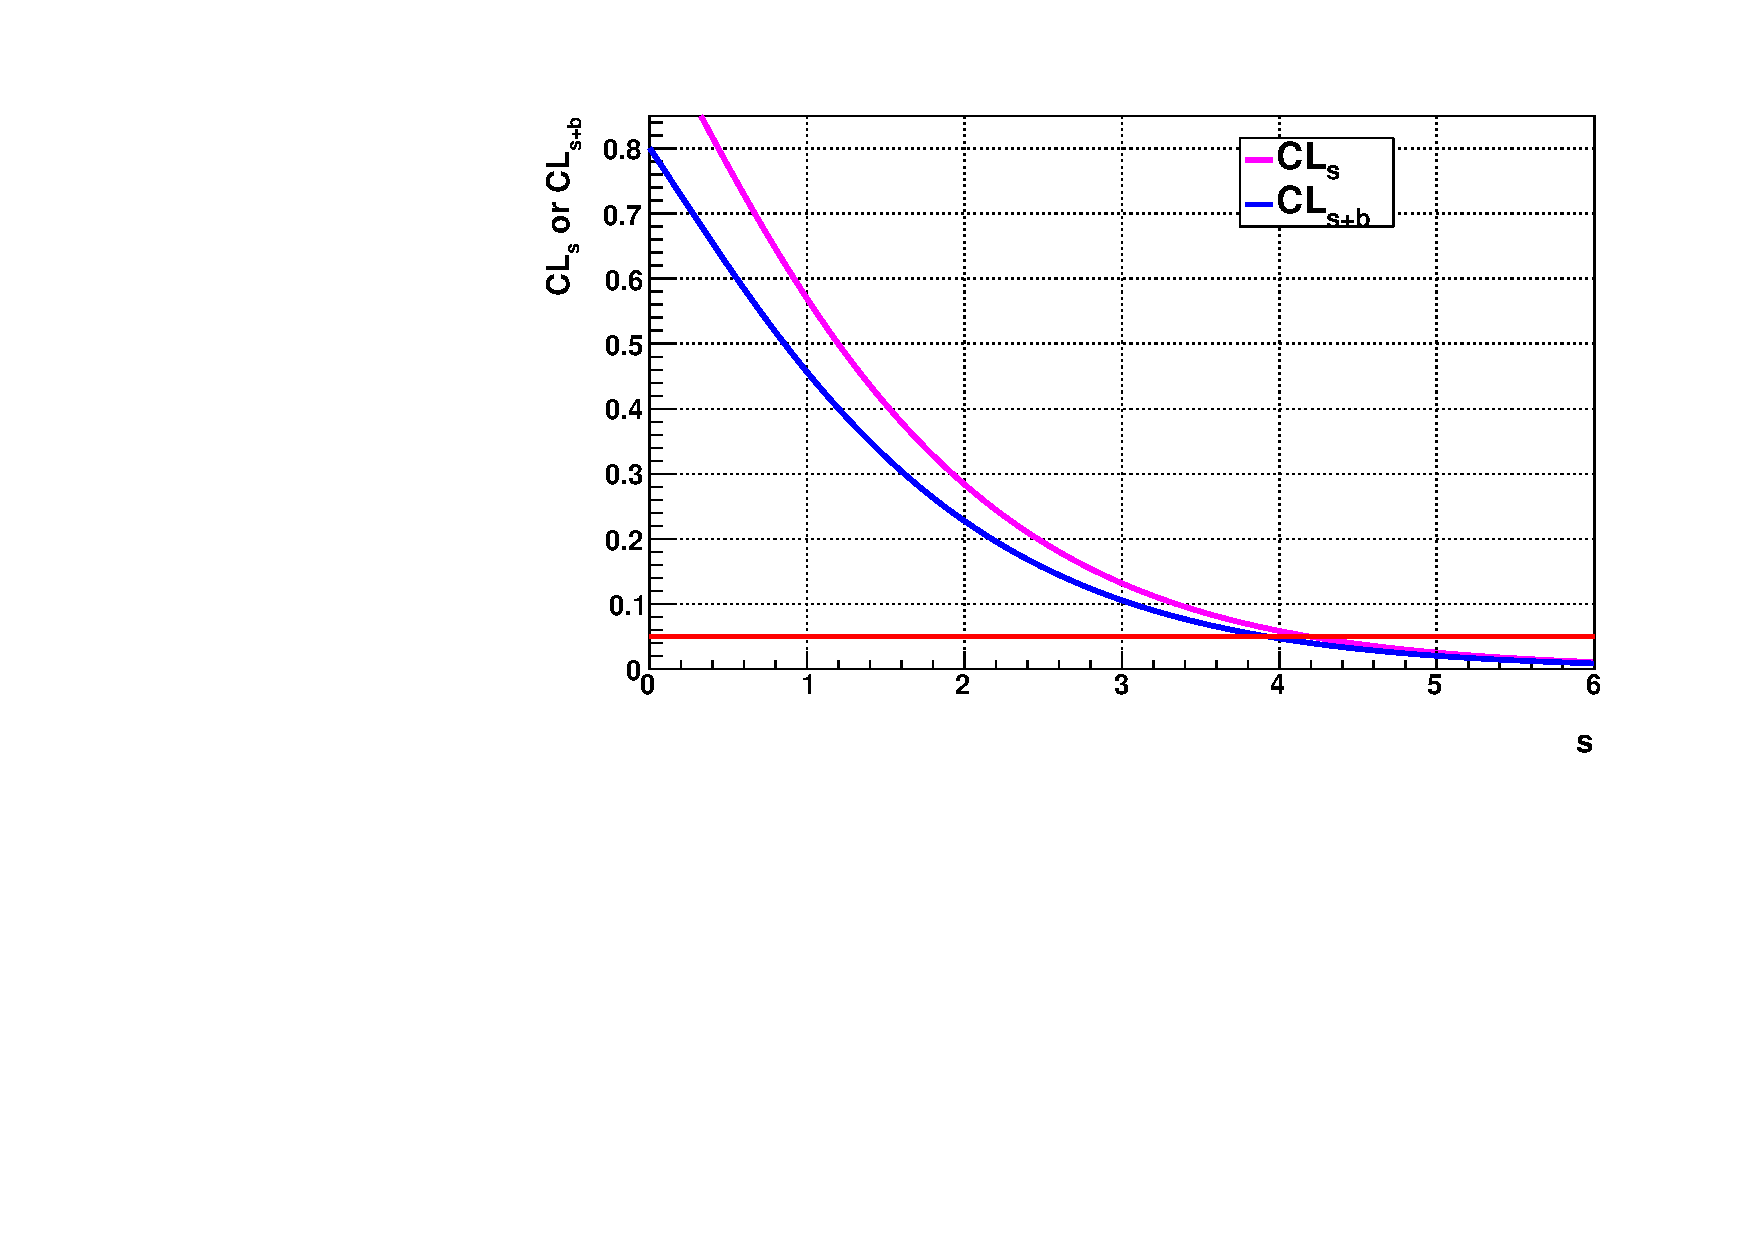
\includegraphics[scale=0.5]{macros/plotCLsbVsS_2}
\end{figure}

\begin{itemize}
\item Remark: upper limit always worse with $CL_{s}$ (in this example:
$s_{\text{up}}=4.19$)
\end{itemize}

\lyxframeend{}\lyxframe{Frequentist solution - $CL_{s}$ method}

\begin{figure}
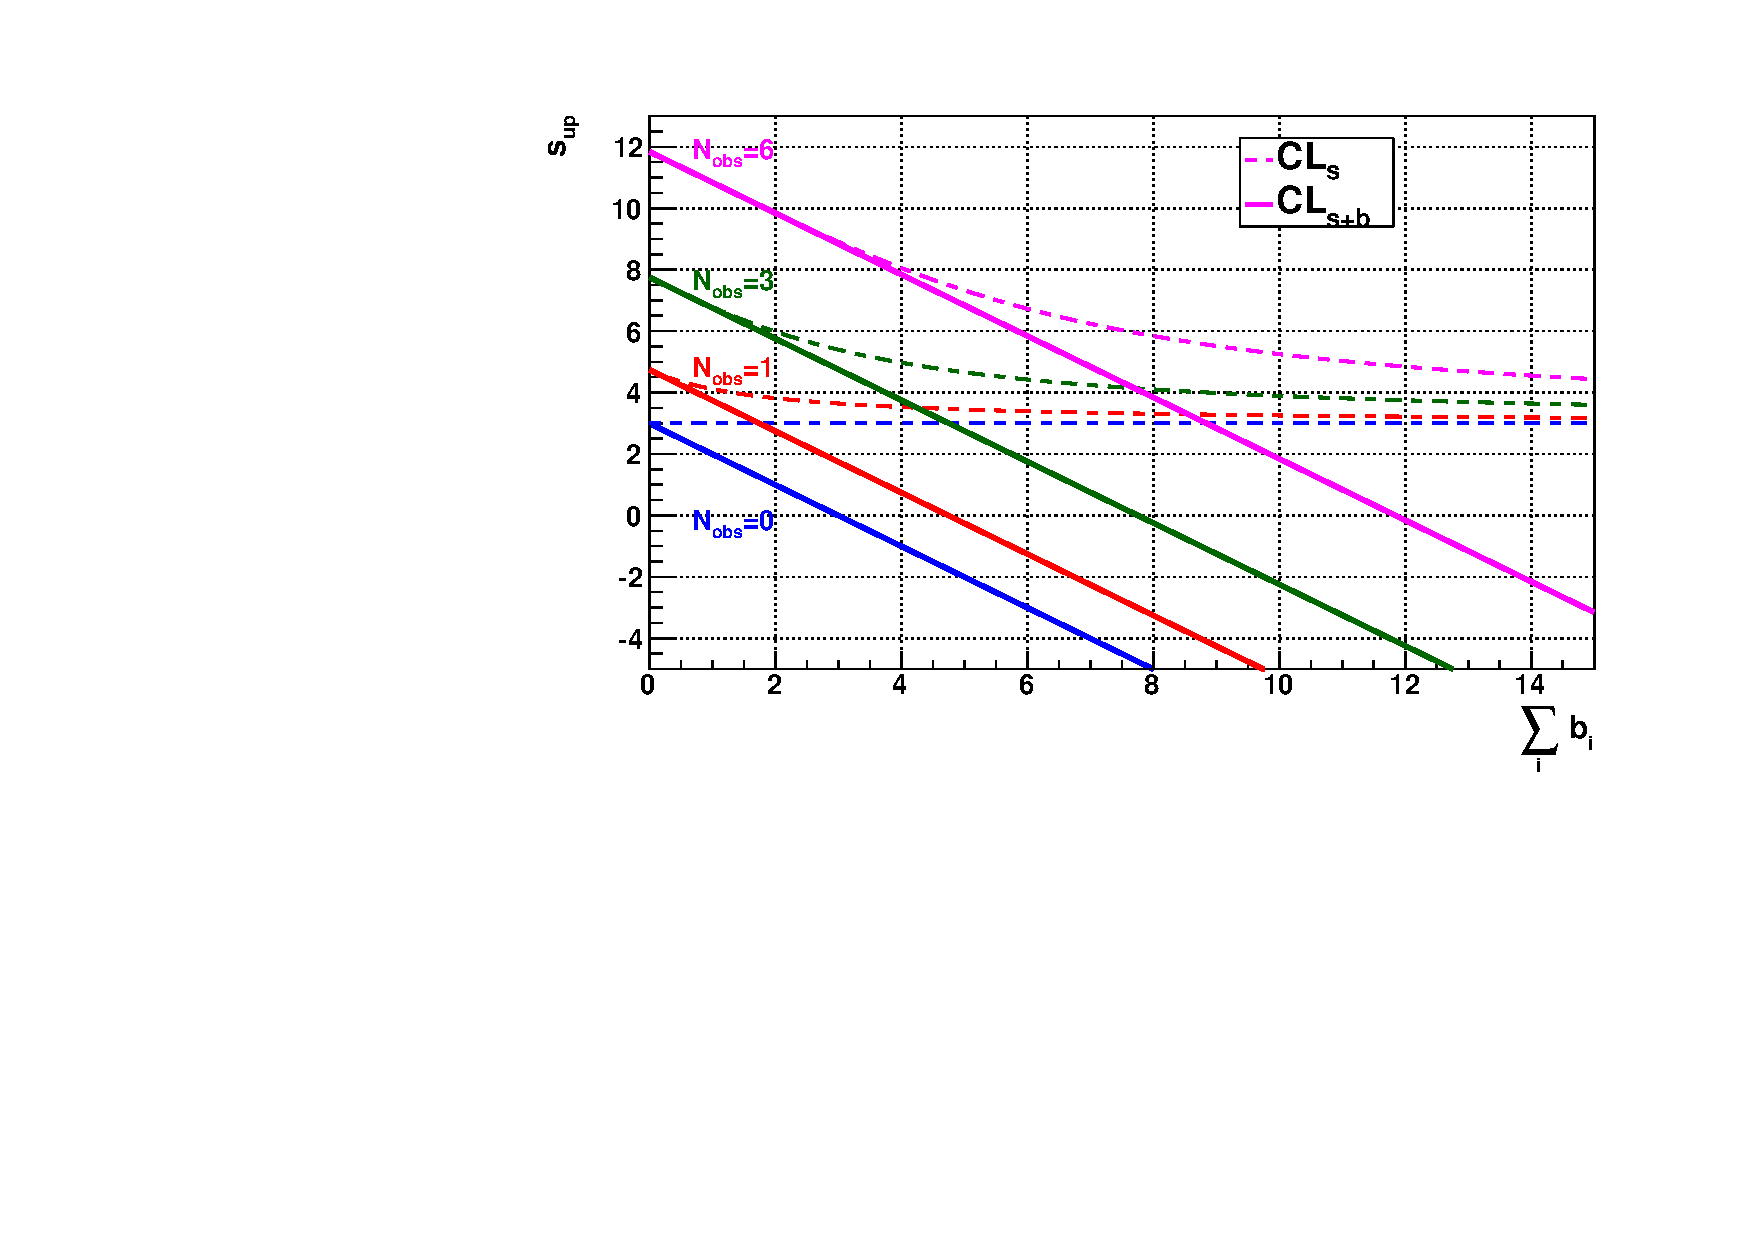
\includegraphics[scale=0.5]{macros/plotLimitVsNbkg_CLsb_2}
\end{figure}



\lyxframeend{}\lyxframe{Frequentist solution}
\begin{itemize}
\item Comments

\begin{itemize}
\item Other solutions than $CL_{s}$ exist to solve $s_{\text{up}}\leq0$
problem (e.g. PCL)
\end{itemize}

\pause{}
\begin{itemize}
\item $CL_{s}$ is the current recommendation in ATLAS
\end{itemize}

\pause{}
\begin{itemize}
\item Previous $CL_{s}$ procedure is what CLsGenerator and McLimit do in
single channel/no uncertainties case
\end{itemize}
\end{itemize}

\lyxframeend{}\lyxframe{Bayesian solution}
\begin{itemize}
\item Reminder: Bayes' theorem


\begin{center}


$P(A|B)=\frac{P(B|A)P(A)}{P(B)}\propto P(B|A)P(A)$ 


\end{center}


$\rightarrow$ Bayesian methods use this theorem to make inference

\end{itemize}

\pause{}
\begin{itemize}
\item Bayes' theorem applied to previous example


\begin{center}


\textcolor{blue}{$\underbrace{f(s|N_{\text{obs}})}_{\text{posterior}}\propto\underbrace{P(N_{\text{obs}}|s)}_{\text{likelihood}}\underbrace{\pi(s)}_{\text{prior}}=\frac{\left(s+\sum\limits _{i}b_{i}\right)^{N_{\text{obs}}}}{N_{\text{obs}}!}e^{-\left(s+\sum\limits _{i}b_{i}\right)}\pi(s)$}


\end{center}

\end{itemize}

\pause{}
\begin{itemize}
\item \textcolor{magenta}{Remark: philosophically very different from frequentist
methods}


\begin{center}


\textbf{\textcolor{magenta}{$\rightarrow$ $s$ considered as a random
variable}}%
\footnote{hence the notation $P(N_{\text{obs}}|s)=P(N_{\text{obs}};s)$%
}


\end{center}

\end{itemize}

\lyxframeend{}\lyxframe{Bayesian solution}
\begin{itemize}
\item Upper limit $s_{\text{up}}$ defined by


\begin{center}


$\boxed{{\displaystyle \int_{0}^{s_{\text{up}}}f(s|N_{\text{obs}})\text{d}s}=1-\alpha}$


\end{center}

\end{itemize}
\vspace*{0.1cm}
\begin{itemize}
\item For previous example ($N_{\text{obs}}=1,$ $\sum b_{i}=0.82$) with
uniform prior
\end{itemize}
\begin{figure}
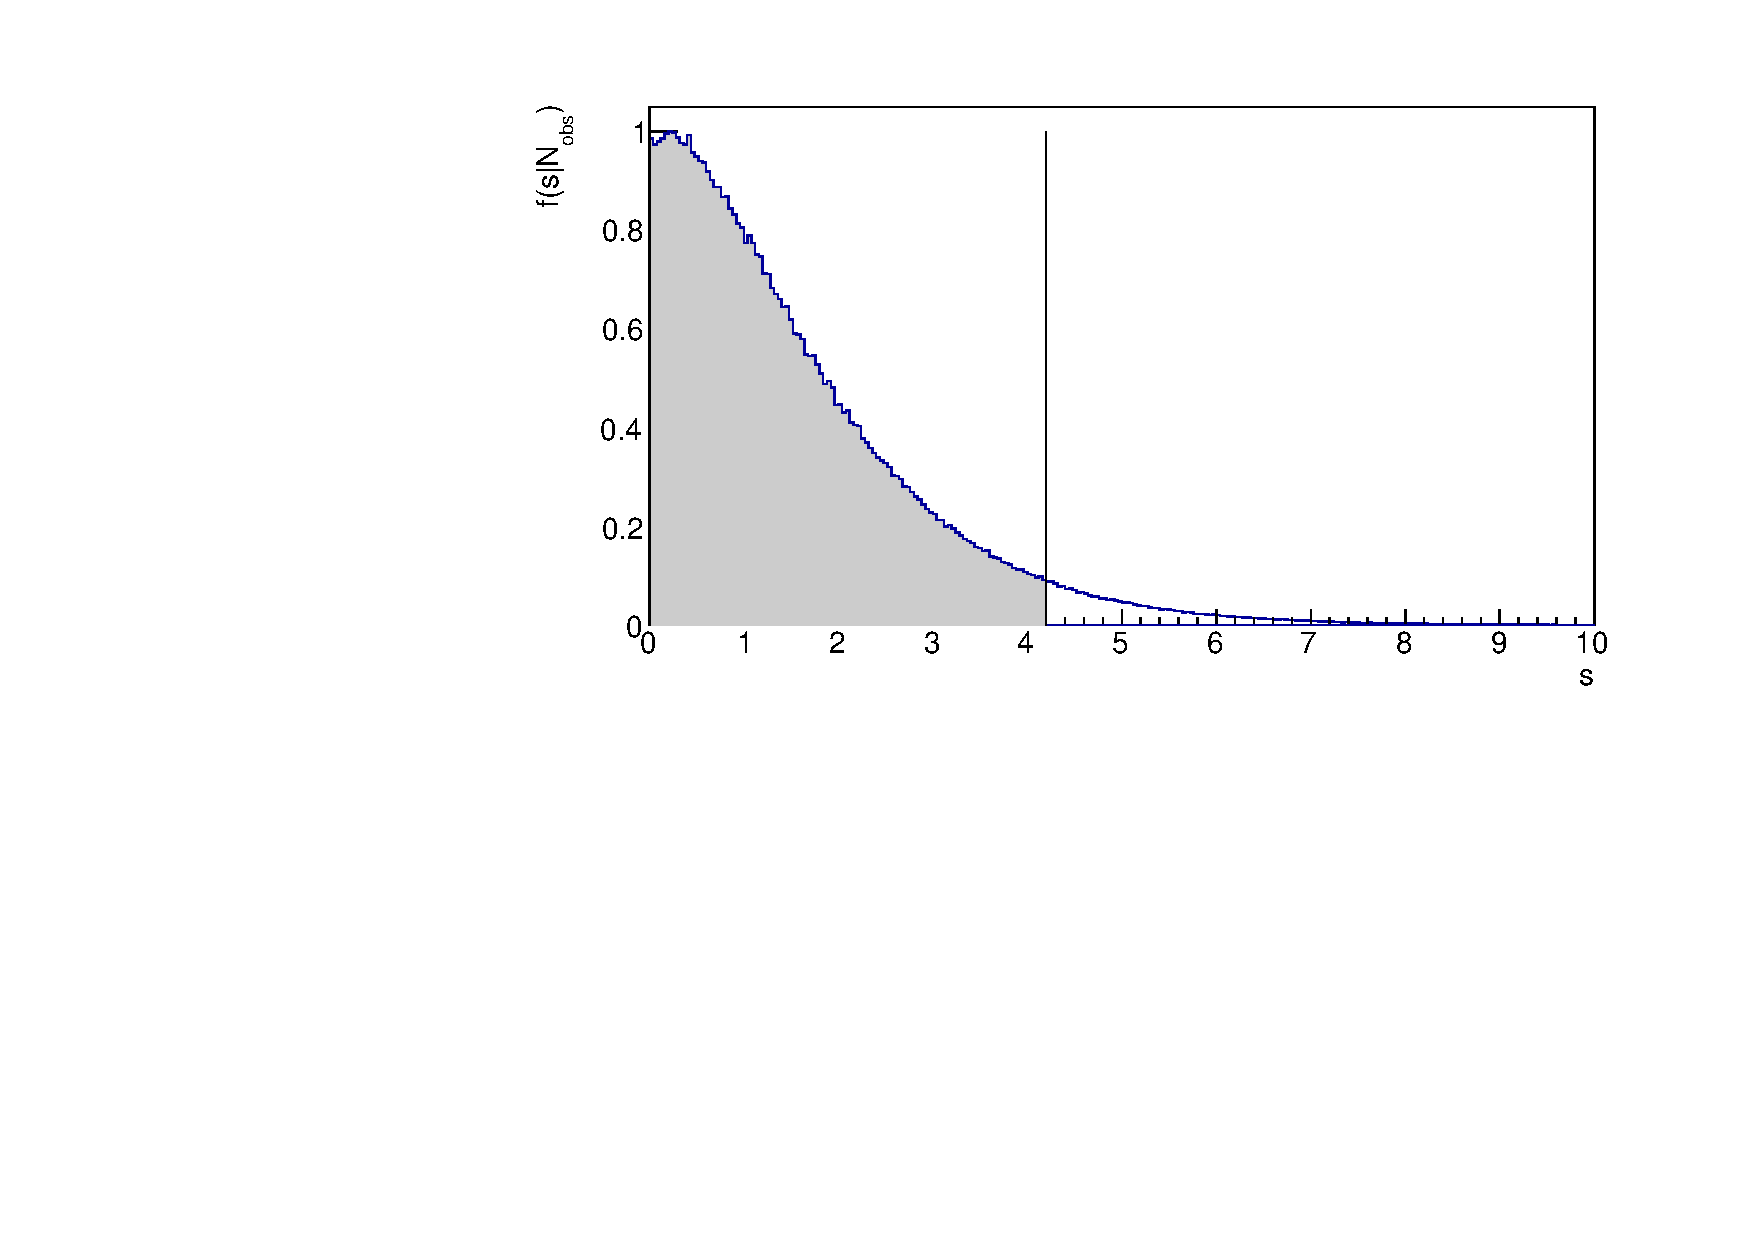
\includegraphics[scale=0.4]{macros/posteriorExample}
\end{figure}


\begin{center}$\rightarrow s_{\text{up}}=4.19$\end{center}


\lyxframeend{}\lyxframe{Frequentist Vs Bayesian}
\begin{itemize}
\item \textcolor{red}{$CL_{s}$ and bayesian with uniform prior strictly
equivalent in simple situation considered here}
\end{itemize}

\pause{}
\begin{itemize}
\item \underline{Proof}


\begin{small}
\begin{itemize}
\item \textrm{$f(s|N_{\text{obs}})=\frac{P(N_{\text{obs}}|s)}{{\displaystyle \int_{0}^{\infty}}P(N_{\text{obs}}|s)\text{ds}}$}


it can be shown that$ $${\displaystyle \int_{0}^{\infty}}P(N_{\text{obs}}|s)ds=CL_{b}$

\item $1-\alpha={\displaystyle \int_{0}^{s_{\text{up}}}f(s|N_{\text{obs}})\text{d}s}=\frac{1}{CL_{b}}{\displaystyle \int_{0}^{s_{\text{up}}}}P(N_{\text{obs}}|s)\text{ds}$


it can be shown that $ $${\displaystyle {\displaystyle \int_{0}^{s_{\text{up}}}}}P(N_{\text{obs}}|s)\text{ds}=CL_{b}-CL_{s+b}(s_{\text{up}})$

\end{itemize}

\begin{center}


$\Rightarrow\alpha=\frac{CL_{s+b}(s_{\text{up}})}{CL_{b}}=CL_{s}(s_{\text{up}})$


\end{center}


\end{small}

\end{itemize}

\lyxframeend{}\lyxframe{Analytical solution}
\begin{itemize}
\item No need to run sophisticated tools to compute previous limits


\begin{center}


$\rightarrow$\textrm{\textcolor{red}{{} }}\textcolor{red}{Analytical
solutions exist}


\end{center}

\end{itemize}

\pause{}
\begin{itemize}
\item Analytical solutions (proofs on next slide)

\begin{itemize}
\item $CL_{s+b}$:


\begin{center}


\textbf{\textcolor{black}{\footnotesize{$\boxed{s_{\text{up}}=0.5\times F_{\chi^{2}}^{-1}\left(1-\alpha;2\left(N_{\text{obs}}+1\right)\right)-\sum b_{i}}$ }}}{\footnotesize \par}


\vspace*{0.2cm}


\texttt{\textcolor{blue}{\footnotesize{0.5{*}ROOT::Math::chisquared\_quantile(1-$\alpha$,2{*}($N_{\text{obs}}$+1))-$b$}}}{\footnotesize \par}


\end{center}

\end{itemize}

\vspace*{0.4cm}
\begin{itemize}
\item $CL_{s}$ and bayesian with uniform prior :


\begin{center}


\textbf{\textcolor{black}{\footnotesize{$\boxed{s_{\text{up}}=0.5\times F_{\chi^{2}}^{-1}\left(1-\alpha\left[1-F_{\chi^{2}}\left(2\sum b_{i};2\left(N_{\text{obs}}+1\right)\right)\right];2\left(N_{\text{obs}}+1\right)\right)-\sum b_{i}}$ }}}{\footnotesize \par}


\end{center}


\texttt{\textcolor{blue}{\footnotesize{0.5{*}ROOT::Math::chisquared\_quantile(1-$\alpha${*}(1-}}}{\footnotesize \par}


\begin{flushright}


\texttt{\textcolor{blue}{\footnotesize{ROOT::Math::chisquared\_cdf(2{*}$b$,2{*}($N_{\text{obs}}$+1))),2{*}($N_{\text{obs}}$+1))-$b$}}}{\footnotesize \par}


\end{flushright}

\end{itemize}
\end{itemize}

\lyxframeend{}\lyxframe{Analytical solution}
\begin{itemize}
\item \underline{Demonstration of previous relations} 

\begin{itemize}
\item Consider first a $CL_{\text{s+b}}$ limit. Upper limit $\mu_{\text{up}}$
at $1-\alpha$ confidence level given by


\begin{center}


$CL_{\text{s+b}}={\displaystyle \sum_{n=0}^{N\text{obs}}}{\cal P}(N;s+\sum b_{i})=\alpha$ 


\end{center}


Poisson c. d. f. given by


\begin{center}


${\displaystyle \sum_{n=0}^{N_{\text{obs}}}{\cal P}}(N;s+\sum b_{i})=1-F_{\chi^{2}}\left(2(s+\sum b_{i});2\left(N_{\text{obs}}+1\right)\right)$ 


\end{center}


Thus


\begin{center}


$ $ \textrm{$s_{\text{up}}=0.5\times F_{\chi^{2}}^{-1}\left(1-\alpha;2\left(N_{\text{obs}}+1\right)\right)-\sum b_{i}$}


\end{center}

\item For $CL_{s}$, just need to replace $\alpha$ by $\alpha\times CL_{\text{b}}$
(since $CL_{b}$ is independant of signal)
\end{itemize}
\end{itemize}

\lyxframeend{}\lyxframe{Remark}
\begin{itemize}
\item Note that previous $CL_{s+b}$ formula is the one used in SS analysis
to set upper limit for samples with yield=0 \vspace*{0.5cm}


\begin{center}


\textrm{$\text{Yield}_{\text{up}}=0.5\times F_{\chi^{2}}^{-1}\left(0.68;2\left(0+1\right)\right)\simeq1.14$}


\end{center}

\end{itemize}

\lyxframeend{}\lyxframe{Summary of methods discussed so far}

\begin{table}
\begin{tabular}{|c|c|c|}
\cline{2-3} 
\multicolumn{1}{c|}{} & \textcolor{black}{\small{Method}} & \textcolor{black}{\small{Comment}}\tabularnewline
\hline 
\multirow{3}{*}{\textcolor{black}{\small{Frequentist}}} & \textcolor{black}{\small{$CL_{s+b}$}} & \textcolor{black}{\small{unphysical when downward fluctuation}}\tabularnewline
\cline{2-3} 
 & \textcolor{black}{\small{$CL_{s}$}} & \textcolor{black}{\small{equivalent to bayesian w/ uniform prior}}\tabularnewline
\cline{2-3} 
 & \textcolor{black}{\small{PCL}} & \textcolor{black}{\small{maybe solution of the future}}\tabularnewline
\hline 
\multirow{2}{*}{\textcolor{black}{\small{Bayesian}}} & \textcolor{black}{\small{Bayesian (uniform prior)}} & \textcolor{black}{\small{equivalent to $CL_{s}$}}\tabularnewline
\cline{2-3} 
 & \textcolor{black}{\small{Bayesian (other priors)}} & \tabularnewline
\hline 
\end{tabular}
\end{table}



\pause{}

\begin{center}$ $

$\rightarrow$ Quite a lot of solutions for such a simple problem

\vspace*{1cm}

\textbf{\textcolor{blue}{It's just the beginning !}}

\end{center}


\lyxframeend{}\lyxframe{Sensitivity of an analysis}
\begin{itemize}
\item Sensitivity of an analysis not given by $s_{\text{up}}$ but by some
quantity measuring by how much $s_{\text{up}}$ differs from some
nominal signal expectation $s_{\text{nom}}$

\begin{itemize}
\item Example: SUSY predicts $s_{\text{nom}}$ sgluon events after selection

\begin{itemize}
\item if $s_{\text{up}}<s_{\text{nom}}$: sgluon excluded
\item if $s_{\text{up}}\text{\ensuremath{\geq}}s_{\text{nom}}$: sgluon
not excluded
\end{itemize}
\end{itemize}
\end{itemize}

\pause{}
\begin{itemize}
\item Sensitivity usually given by 


\begin{center}


\textcolor{red}{$\mu_{\text{up}}=\frac{s_{\text{up}}}{s_{\text{nom}}}$}


\end{center}


If $\mu_{\text{up}}\gg1$, analysis not sensitive 

\end{itemize}

\lyxframeend{}\lyxframe{Comments on historical $\mu_{\text{up}}=1.64\sqrt{b}/s_{\text{nom}}$}
\begin{itemize}
\item In order to compute sensitivities fast, people sometimes use


\begin{center}


\textcolor{red}{$\mu_{\textup{up}}=1.64\frac{\sqrt{b}}{s_{\text{nom}}}\qquad$}
\textcolor{black}{\footnotesize{($b:$ total background)}}{\footnotesize \par}


\end{center}

\item From this formula one often predicts that sensitivity should scale
as $1/\sqrt{\text{Lumi}}$
\end{itemize}

\pause{}

\begin{center}

\textcolor{blue}{$\rightarrow$ Where does this come from ? }

\textcolor{blue}{$\rightarrow$ What approximations are behind ? }

\textcolor{blue}{$\rightarrow$ Can we do better ?}

\textcolor{blue}{$\rightarrow$ Is the $1/\sqrt{\text{Lumi}}$ scaling
correct ?}

\end{center}


\lyxframeend{}\lyxframe{Gaussian approximation}
\begin{itemize}
\item Analytical solution in gaussian approximation

\begin{itemize}
\item When $s+\sum b_{i}$ is large, poisson $\simeq$ gaussian with $\sigma=\sqrt{s+\sum b_{i}}$
\end{itemize}

\pause{}
\begin{itemize}
\item We can show that, for $CL_{s+b}$ (see next slide)


\begin{center}


\textrm{$\boxed{{s_{\text{up}}=N_{\text{obs}}-\sum b_{i}+\frac{\left[\Phi^{-1}(1-\alpha)\right]^{2}}{2}\left[1+\sqrt{1+4\frac{N_{\text{obs}}}{\left[\Phi^{-1}(1-\alpha)\right]^{2}}}\right]}}$}


\end{center}


where $\Phi$ is the c. d. f. of the standard normal distribution

\end{itemize}
\end{itemize}

\lyxframeend{}\lyxframe{Gaussian approximation - Demonstration}
\begin{itemize}
\item For $CL_{s+b}$, we have by definition


\begin{center}


$CL_{\text{s+b}}={\displaystyle \int_{0}^{N_{\text{{obs}}}}G\left(N;s_{\text{up}}+\sum b_{i},\sqrt{{s_{\text{up}}+\sum b_{i}}}\right)}\text{d}N=\alpha$ 


$\text{\ensuremath{\Rightarrow}}$ ${\displaystyle \int_{0}^{\frac{N_{\text{obs}}-(s_{\text{up}}+\sum b_{i})}{\sqrt{s_{\text{up}}+\sum b_{i}}}}G(N;0,1)}\text{d}N=\alpha$ 


$\text{\ensuremath{\Rightarrow}}$ $\Phi\left(\frac{N_{\text{\text{obs}}}-(s_{\text{up}}+\sum b_{i})}{\sqrt{s_{\text{up}}+\sum b_{i}}}\right)=\alpha$ 


$\Rightarrow N_{\text{obs}}-(s_{\text{up}}+\sum b_{i})=-\sqrt{s_{\text{up}}+\sum b_{i}}\times\Phi^{-1}(1-\alpha)$ 


\end{center}


Solving for $s_{\text{up}}$ gives expression on previous slide

\item For $CL_{s}$, just need to replace $\alpha$ by $\alpha\times\underbrace{\Phi\left(\frac{N_{\text{obs}-\sum b_{i}}}{\sqrt{\sum b_{i}}}\right)}_{CL_{b}}$
(as for Poisson)
\end{itemize}

\lyxframeend{}\lyxframe{Comments on historical $\mu_{\text{up}}=1.64\sqrt{b}/s_{\text{nom}}$}

\begin{center}

\textrm{$\boxed{{\mu_{\text{up}}=\frac{N_{\text{obs}}-\sum b_{i}}{s_{\text{nom}}}+\frac{\left[\Phi^{-1}(1-\alpha)\right]^{2}}{2s_{\text{nom}}}\left[1+\sqrt{1+4\frac{N_{\text{obs}}}{\left[\Phi^{-1}(1-\alpha)\right]^{2}}}\right]}}$$\quad(\star)$}

\end{center}


\pause{}
\begin{itemize}
\item Let's assume that

\begin{enumerate}
\item $N_{\text{obs}}=\sum b_{i}$ (i.e. expected limit)
\item $\sum b_{i}\gg\left[\Phi^{-1}(1-\alpha)\right]^{2}/4$ 

\begin{itemize}
\item note that $\Phi^{-1}(1-\alpha)=1.64$ for $\alpha=0.05$, corresponding
to $\sum b_{i}\gg0.7$
\item this assumption corresponds more or less to the gaussian approx.
\end{itemize}
\end{enumerate}

Then, one sees directly from $(\star)$ that


\begin{center}


$\boxed{{\mu_{\text{up}}\simeq\Phi^{-1}(1-\alpha)\frac{\sqrt{\sum b_{i}}}{s_{\text{nom}}}=1.64\frac{\sqrt{\sum b_{i}}}{s_{\text{nom}}}}}$


\end{center}

\end{itemize}

\lyxframeend{}\lyxframe{Comments on historical $\mu_{\text{up}}=1.64\sqrt{b}/s_{\text{nom}}$}
\begin{itemize}
\item \textcolor{blue}{Where does this come from ? What approximations are
behind ?}


\pause{}


$\rightarrow$ $CL_{s+b}$ method under gaussian approximation

\end{itemize}
\vspace*{0.5cm}


\pause{}
\begin{itemize}
\item \textcolor{blue}{Can we do better ?}


\pause{}


$\rightarrow$ Yes: \textcolor{red}{use analytical $CL_{s}$ poisson
solution (no more complicated to use and more correct)}


\begin{center}


\textbf{\textcolor{black}{\footnotesize{$\boxed{s_{\text{up}}=0.5\times F_{\chi^{2}}^{-1}\left(1-\alpha\left[1-F_{\chi^{2}}\left(2\sum b_{i};2\left(N_{\text{obs}}+1\right)\right)\right];2\left(N_{\text{obs}}+1\right)\right)-\sum b_{i}}$ }}}{\footnotesize \par}


\end{center}


\texttt{\textcolor{blue}{\footnotesize{0.5{*}ROOT::Math::chisquared\_quantile(1-$\alpha${*}(1-}}}{\footnotesize \par}


\begin{flushright}


\texttt{\textcolor{blue}{\footnotesize{ROOT::Math::chisquared\_cdf(2{*}$b$,2{*}($N_{\text{obs}}$+1))),2{*}($N_{\text{obs}}$+1))-$b$}}}{\footnotesize \par}


\end{flushright}

\end{itemize}

\lyxframeend{}\lyxframe{Comments on historical $\mu_{\text{up}}=1.64\sqrt{b}/s_{\text{nom}}$}
\begin{itemize}
\item Consider example with $b=0.82$, $s_{\text{nom}}=2.49$ for Lumi$=1$
\end{itemize}
\begin{figure}
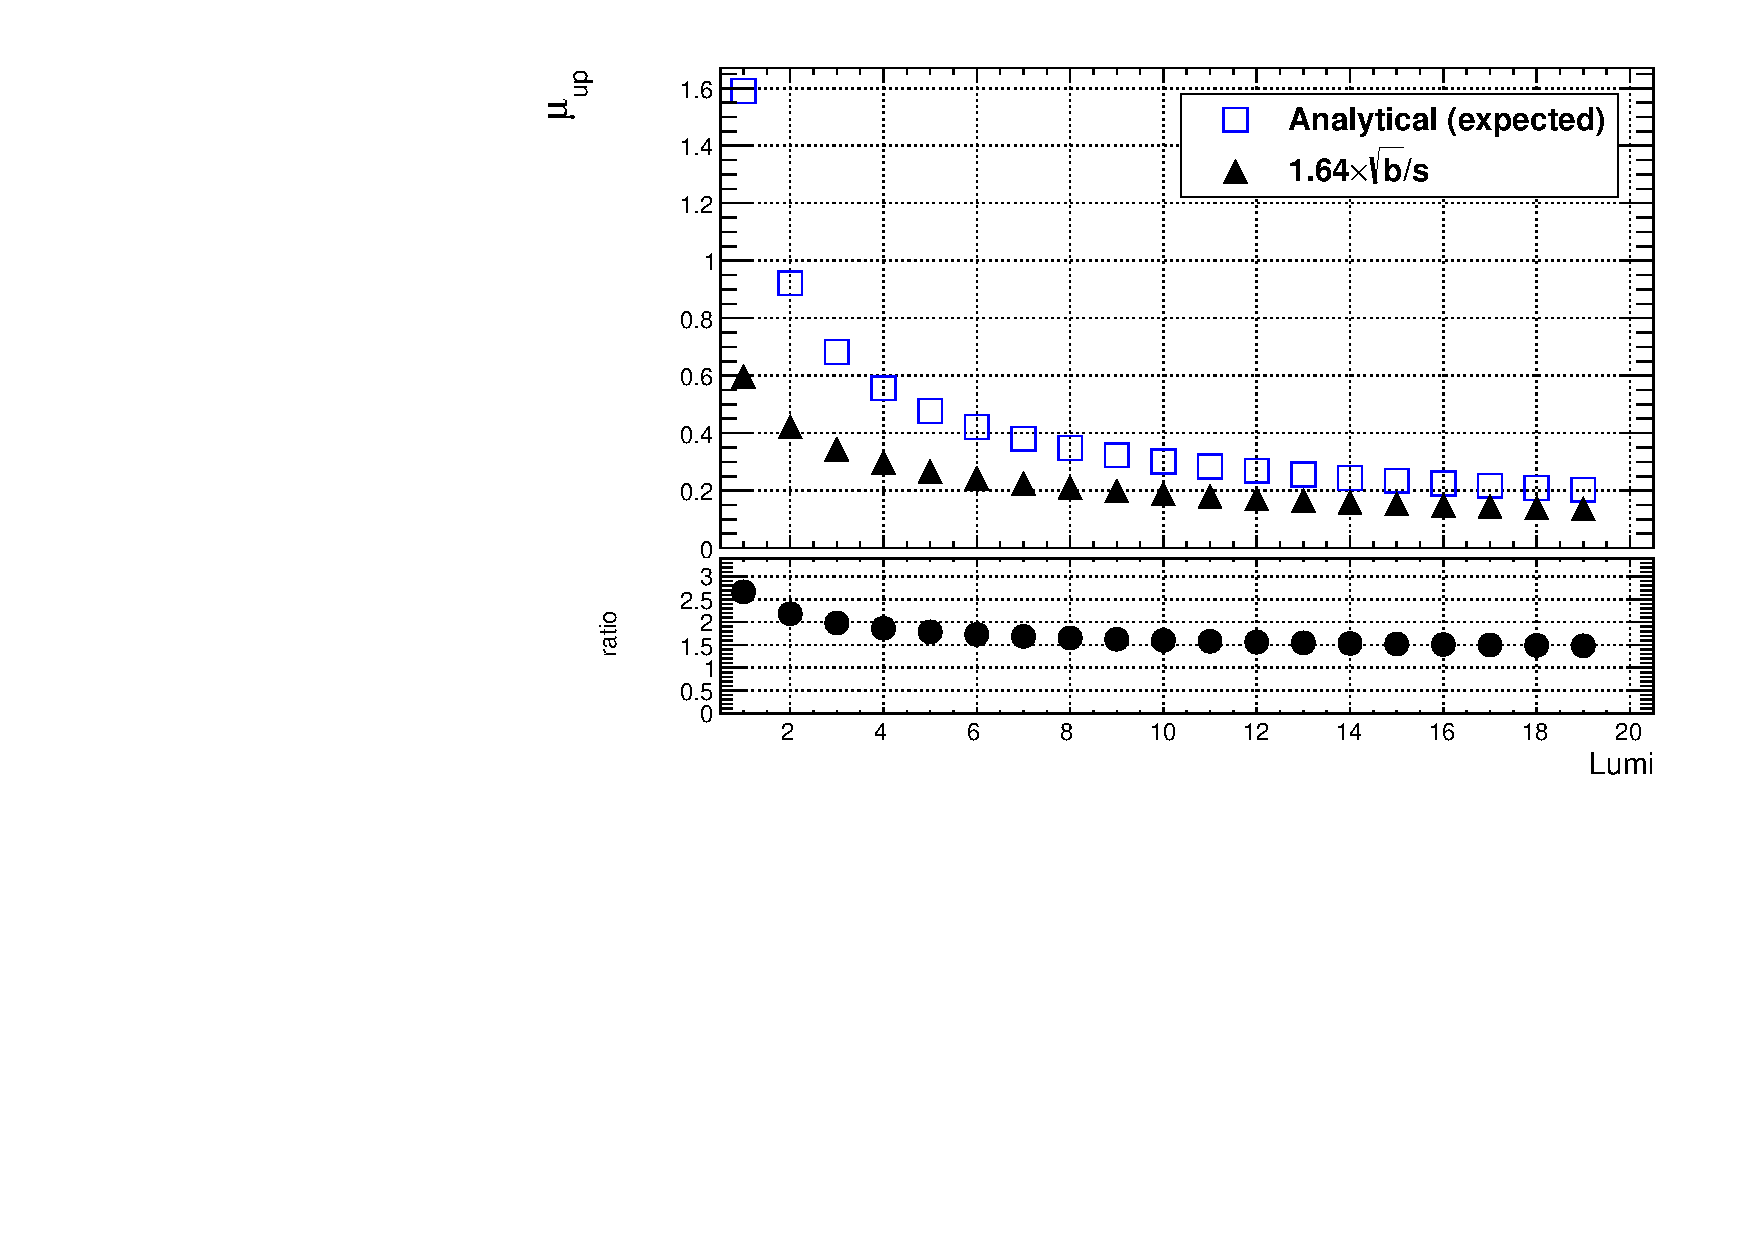
\includegraphics[scale=0.4]{macros/plotLimitVsLumiAnalyticalBadApprox1}
\end{figure}



\lyxframeend{}\lyxframe{Comments on historical $\mu_{\text{up}}=1.64\sqrt{b}/s_{\text{nom}}$}
\begin{itemize}
\item \textcolor{blue}{Is the $1/\sqrt{\text{Lumi}}$ scaling correct ?}


$\rightarrow$ As before: $b=0.82$, $s_{\text{nom}}=2.49$ for Lumi$=1$


\begin{figure}
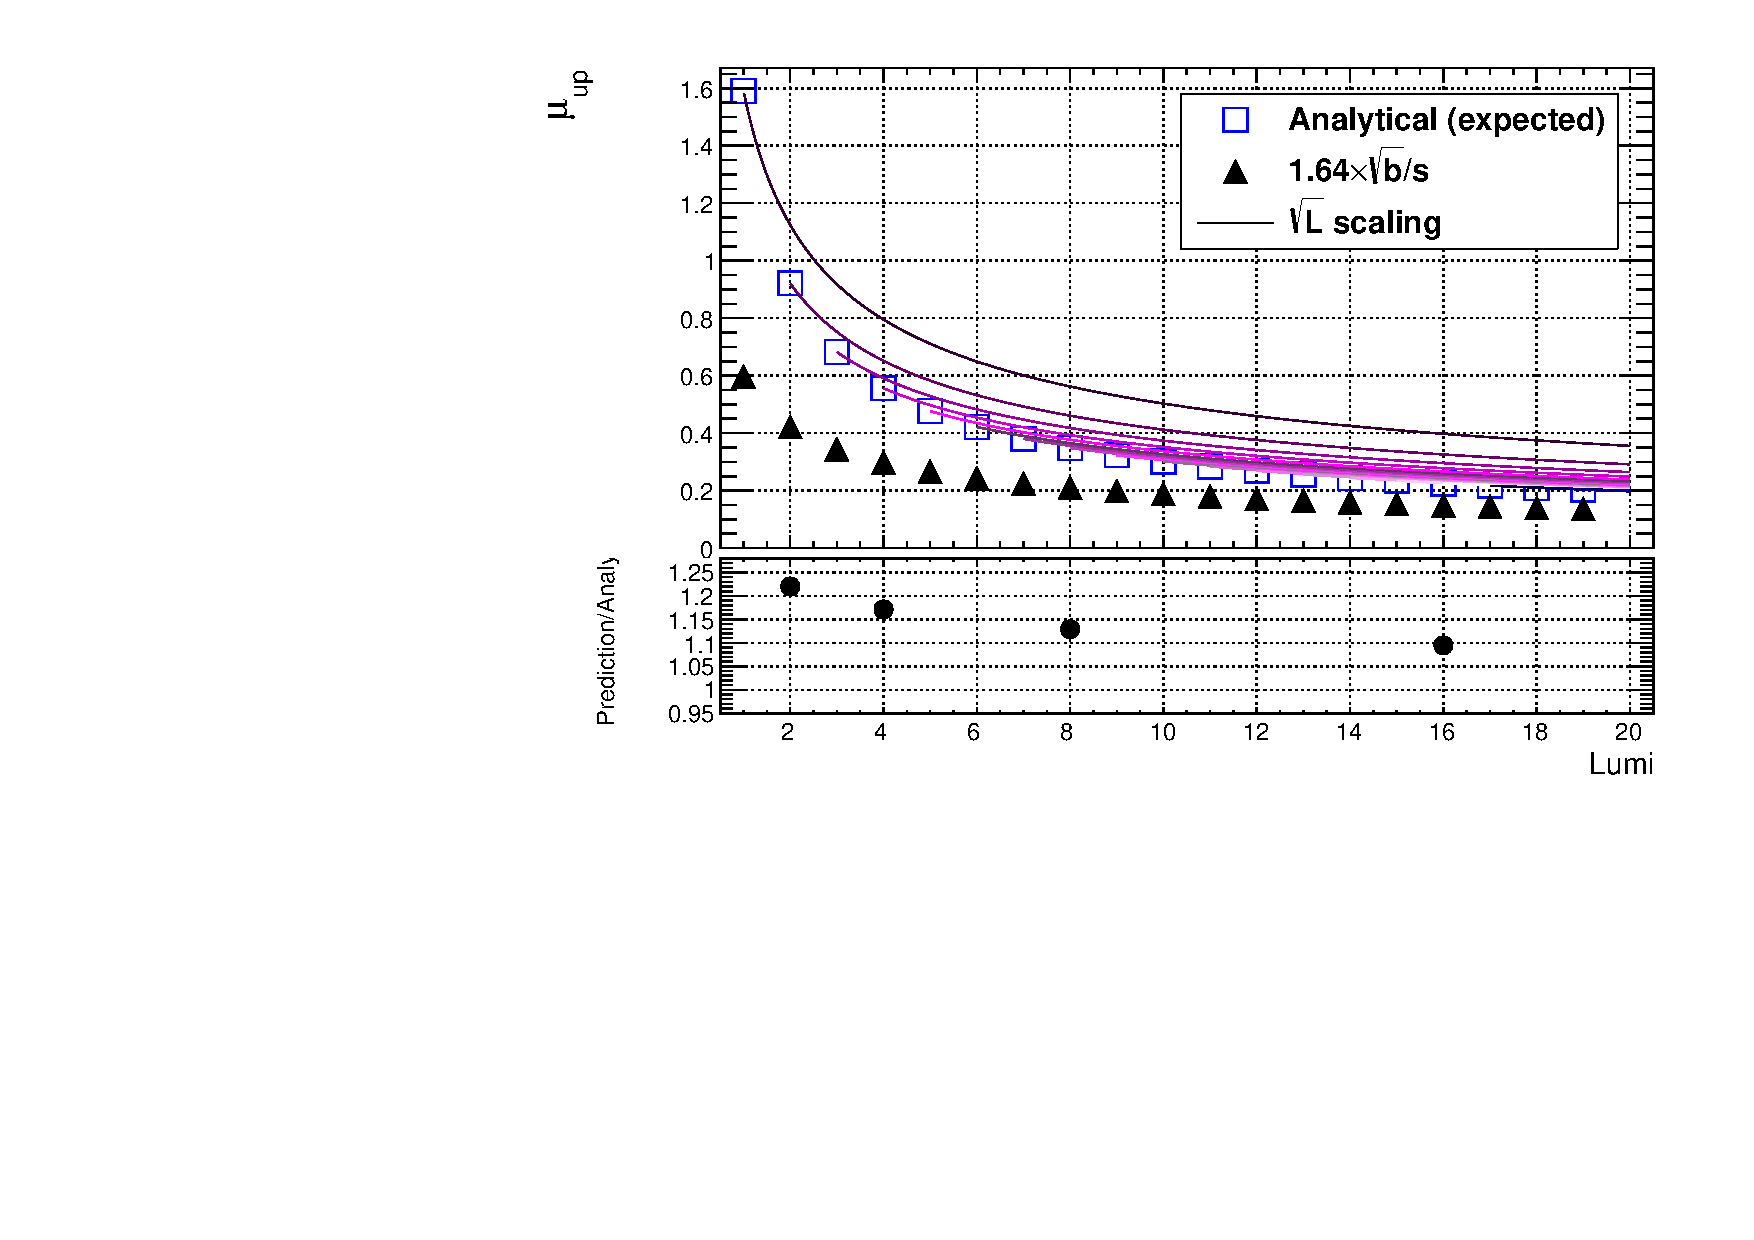
\includegraphics[scale=0.37]{macros/plotLimitVsLumiAnalyticalBadApprox2}
\end{figure}



\begin{center}


$\Rightarrow$ $1/\sqrt{\text{Lumi}}$ scaling rather good approximation
when number of events not too small 


\end{center}

\end{itemize}

\lyxframeend{}\lyxframe{Softwares}
\begin{itemize}
\item No softwares needed, use analytical (unless you want bayesian w/ non-uniform
prior or profile likelihood)
\end{itemize}

\lyxframeend{}\lyxframe{Validation of CLsGenerator and BayesianMCMC}
\begin{itemize}
\item Use analytical solution to validate CLsGenerator and BayesianMCMC 
\end{itemize}
\vspace*{0.2cm}

\begin{minipage}[c]{0.5\columnwidth}%
\begin{figure}
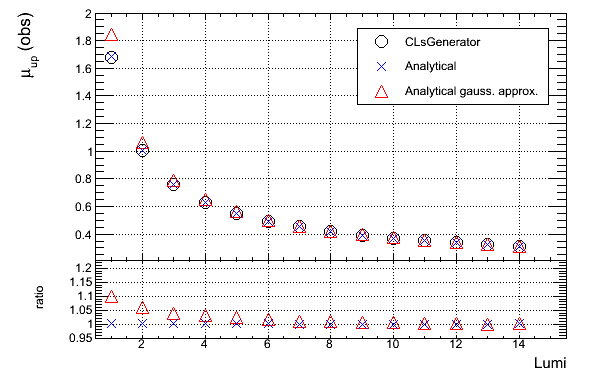
\includegraphics[scale=0.3]{figures/cLimitVsLumi1}
\end{figure}
%
\end{minipage}%
\begin{minipage}[c]{0.4\columnwidth}%
\begin{figure}
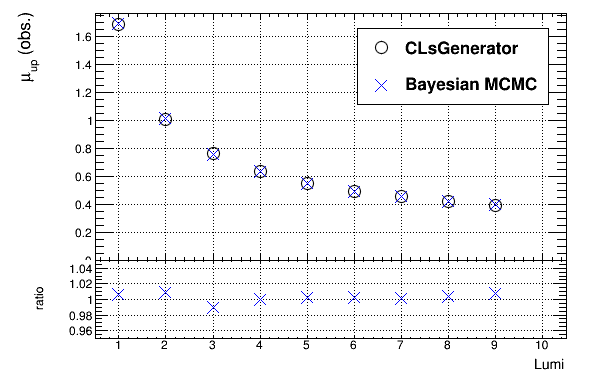
\includegraphics[scale=0.3]{figures/cLimitCLsGenVsBayesian}
\end{figure}
%
\end{minipage}

\vspace*{0.2cm}

\begin{center}

$\rightarrow$ CLsGenerator and BayesianMCMC validated in single channel
- no uncertainties case

\end{center}


\lyxframeend{}\section{Multiple channels - No uncertainties}


\lyxframeend{}\lyxframe{}

\begin{center}
\vspace*{2cm}
{\Large Multiple channels - No uncertainties}
\end{center}


\lyxframeend{}\lyxframe{Generalizing frequentist methods}
\begin{itemize}
\item Methods presented in simple ``Single channel - No uncertainties''
case can be used as prototypes for more general cases
\end{itemize}

\pause{}
\begin{itemize}
\item What we did previously was to

\begin{enumerate}
\item Pick variable with discrimating power between background and signal+background
hypothesis\vspace*{0.2cm}
\item Determine distribution of this variable\vspace*{0.2cm}
\item Compute $p-values$ as a function of signal yield $s$\vspace*{0.2cm}
\item Determine upper limit $s_{\text{up}}$\vspace*{0.2cm}
\end{enumerate}
\item All frequentist methods based on this general scheme
\end{itemize}

\lyxframeend{}\lyxframe{Generalizing frequentist methods}

\begin{figure}
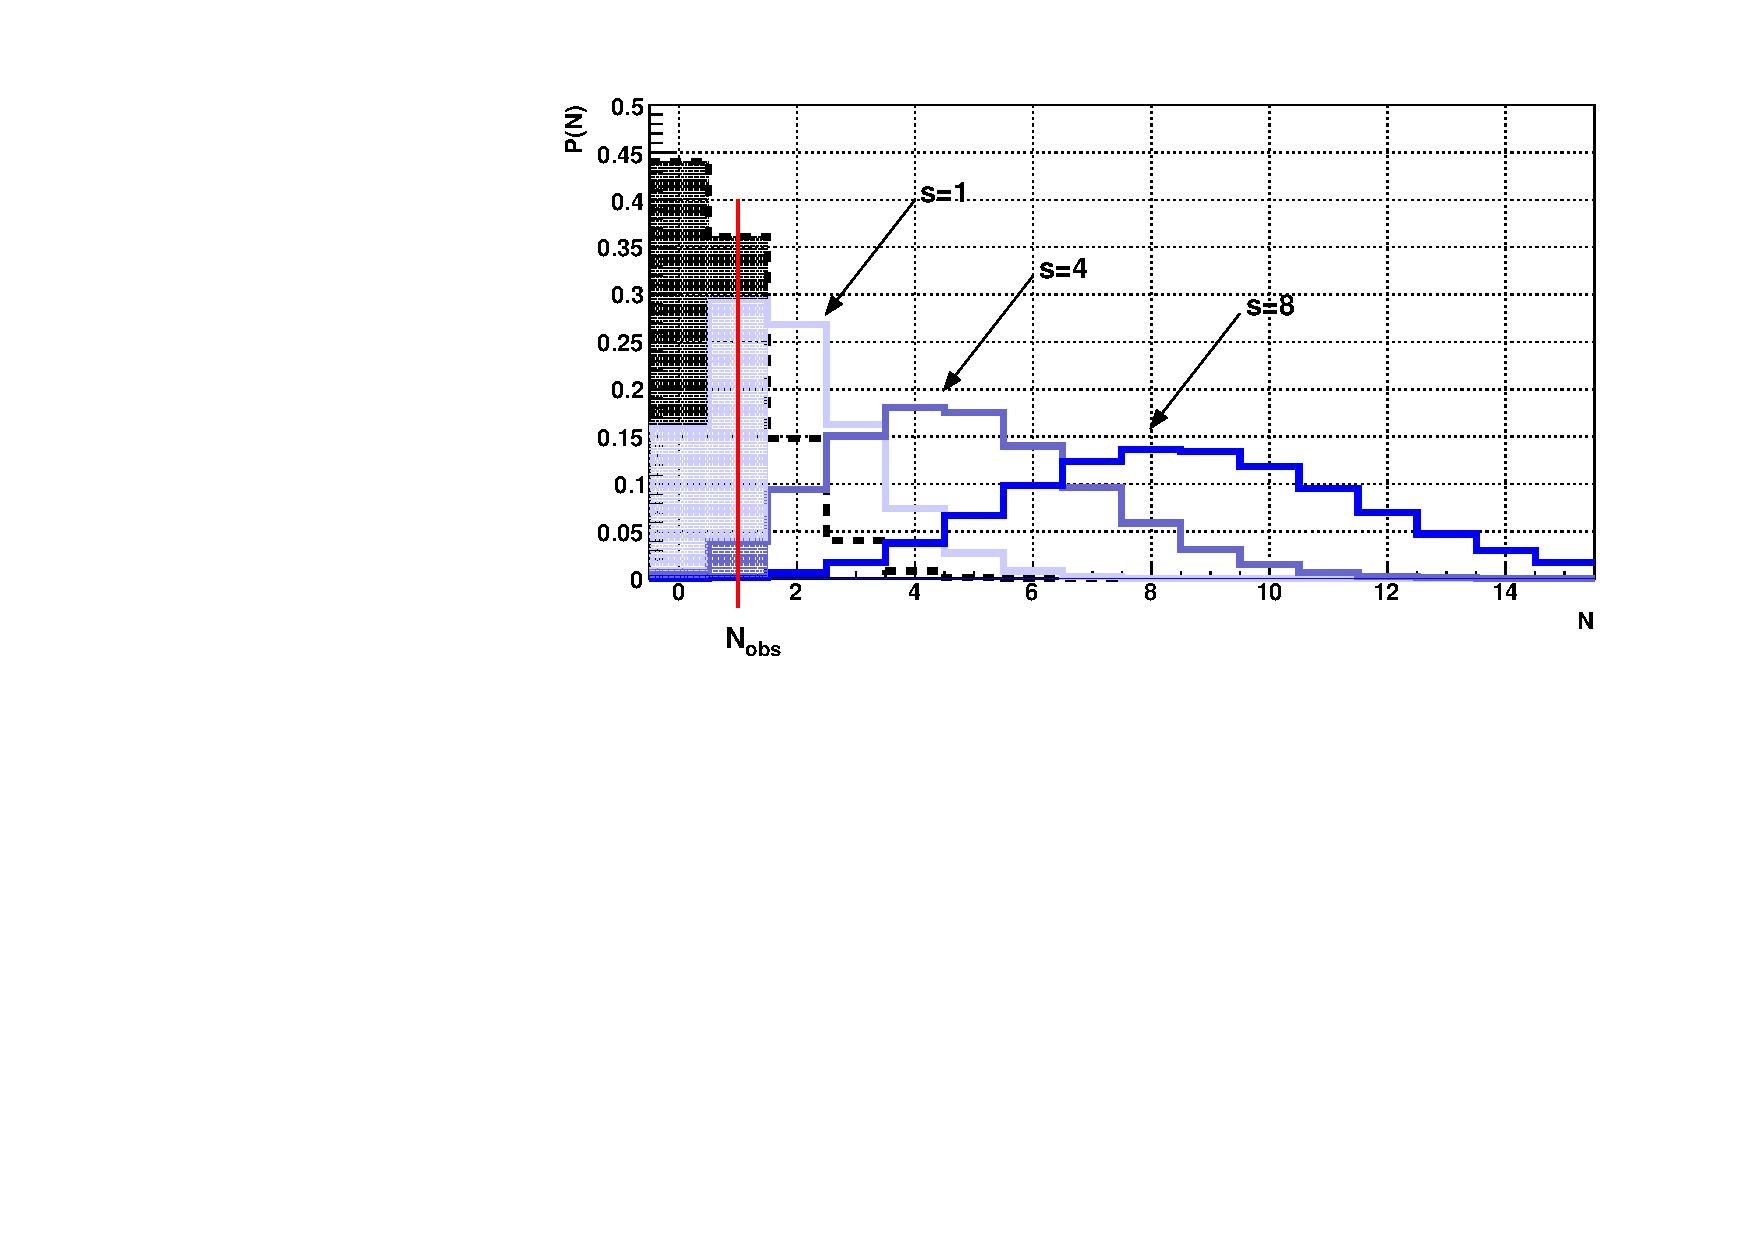
\includegraphics[scale=0.5]{macros/poissonDistributionSig8PvalBkg}
\end{figure}



\lyxframeend{}\lyxframe{Generalizing frequentist methods - Test statistic}
\begin{itemize}
\item \textcolor{blue}{How to choose variable ?}


\pause{\vspace*{0.2cm}}
\begin{itemize}
\item Need single discriminating variable summarizing information from all
channels


\pause{\vspace*{0.2cm}}


$\rightarrow$ Can't use observed yield anymore


\pause{\vspace*{0.2cm}}


$\rightarrow$ \textcolor{red}{Use likelihood based variables}\vspace*{0.2cm}


\begin{center}


$\boxed{{\cal L}_{\text{joint}}={\displaystyle \prod_{c:\text{channels}}{\cal L}_{\text{c}}}}$


\end{center}

\end{itemize}

\pause{\vspace*{0.2cm}}
\begin{itemize}
\item Discriminating power as good as possible\vspace*{0.2cm}


$\rightarrow$ \textcolor{red}{Likelihood ratios are a good choice
(Neyman-Pearson Lemma)}

\end{itemize}
\end{itemize}

\pause{}
\begin{itemize}
\item Terminology: this variable is called \textcolor{red}{test statistic}
or simply \textcolor{red}{test}
\end{itemize}

\lyxframeend{}\lyxframe{Generalizing frequentist methods - Test statistic}
\begin{itemize}
\item Once a test is chosen, apply the rest of the procedure as before
\end{itemize}
\begin{figure}
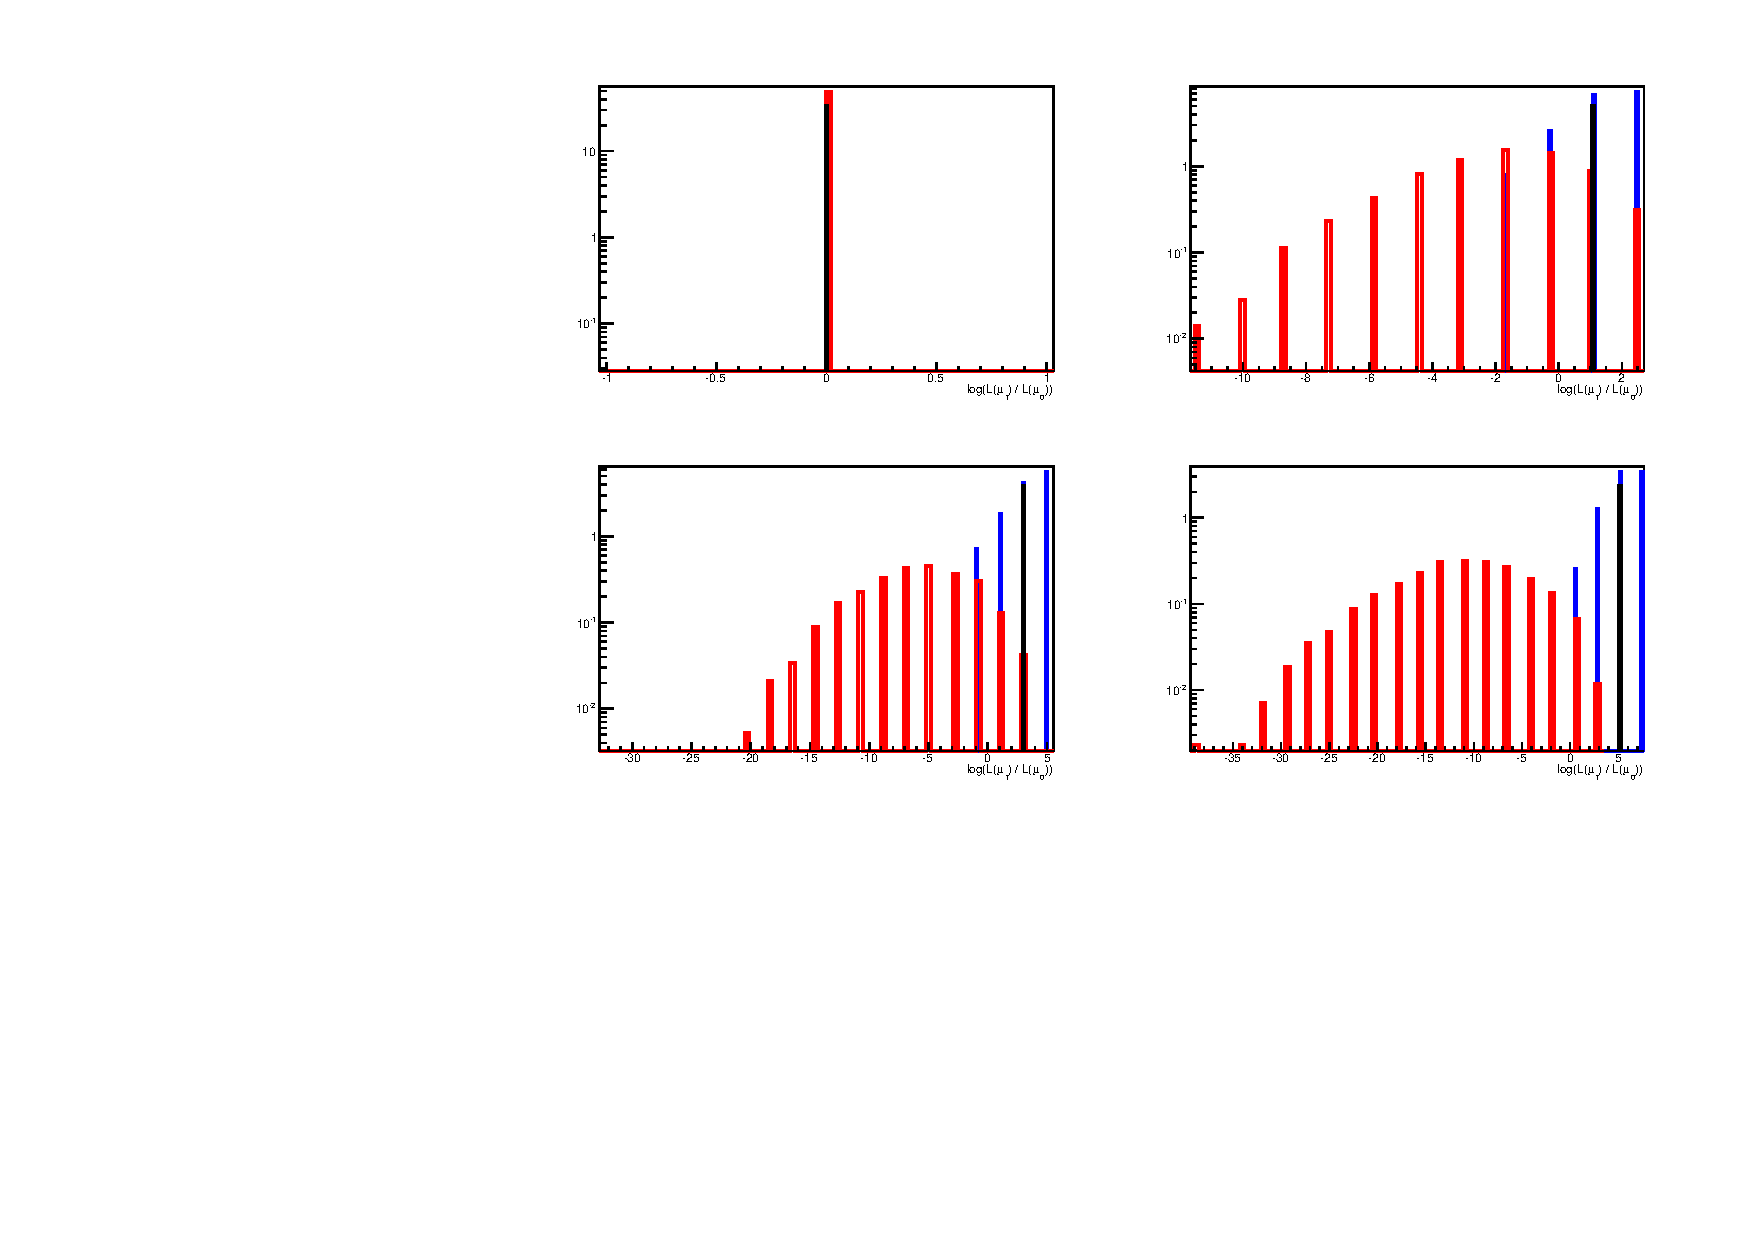
\includegraphics[scale=0.5]{figures/plotTestStatVariousMuExample1}
\end{figure}



\lyxframeend{}\lyxframe{Generalizing frequentist methods - Test statistic}
\begin{itemize}
\item Once a test is chosen, apply the rest of the procedure as before
\end{itemize}
\begin{figure}
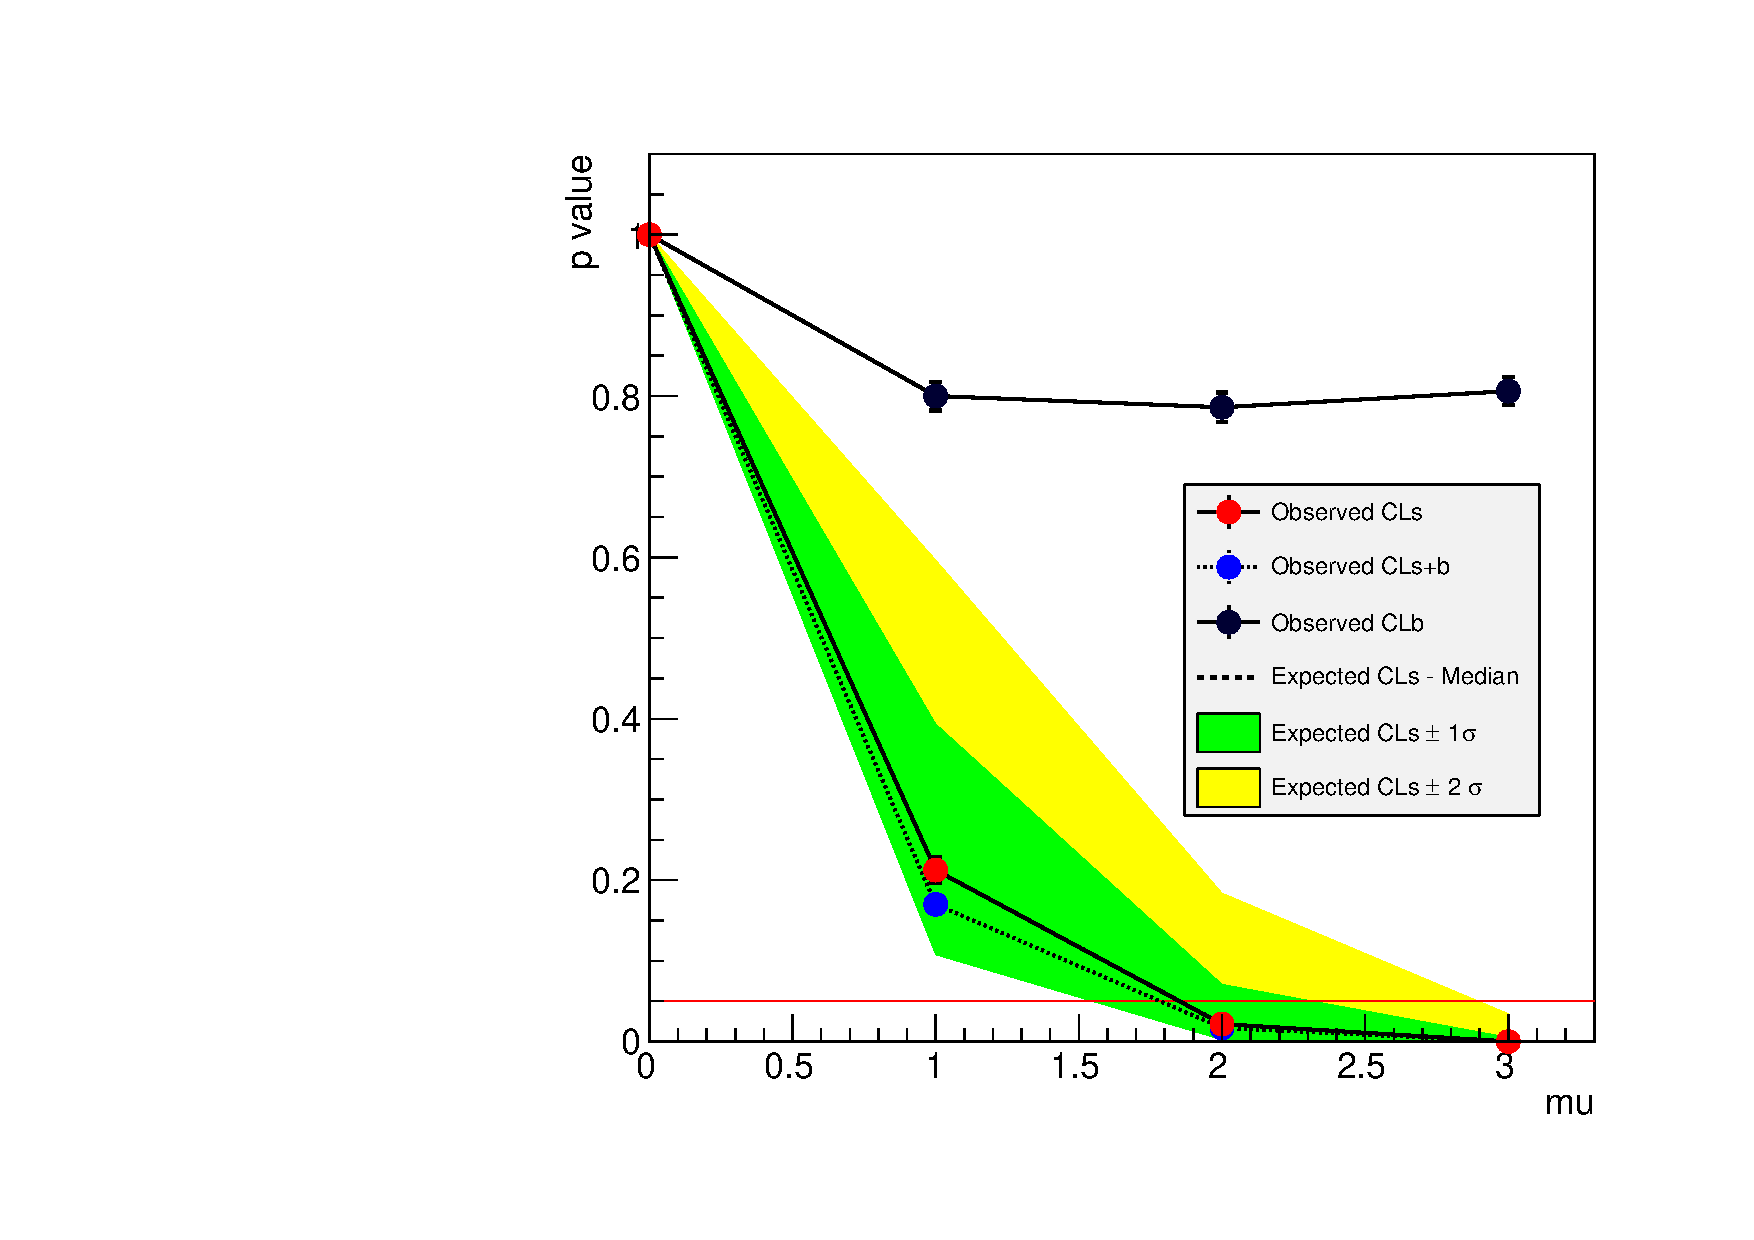
\includegraphics[scale=0.35]{figures/plotTestStatVariousMuExample2}
\end{figure}



\lyxframeend{}\lyxframe{Common test statistics}

\begin{table}
\begin{tabular}{|c|c|c|}
\hline 
Test statistic & Comment & Software\tabularnewline
\hline 
\noalign{\vskip\doublerulesep}
$q_{\mu}=-2\ln\frac{{\cal L}(\mu)}{{\cal L}(\mu=0)}$ & \multirow{2}{*}{\textcolor{black}{\scriptsize{Used at LEP, Tevatron, LHC}}} & \multirow{2}{*}{\textcolor{black}{\scriptsize{McLimit, CLsGenerator, RooStats}}}\tabularnewline[\doublerulesep]
\noalign{\vskip\doublerulesep}
\noalign{\vskip\doublerulesep}
(\textcolor{black}{\footnotesize{simple likelihood ratio}}) &  & \tabularnewline[\doublerulesep]
\noalign{\vskip\doublerulesep}
\hline 
\noalign{\vskip\doublerulesep}
$q_{\mu}'=-2\ln\frac{{\cal L}(\mu)}{{\cal L}(\hat{\mu})}$ & \multirow{2}{*}{\textcolor{black}{\scriptsize{Used at LHC}}} & \multirow{2}{*}{\textcolor{black}{\scriptsize{RooStats}}}\tabularnewline[\doublerulesep]
\noalign{\vskip\doublerulesep}
\noalign{\vskip\doublerulesep}
(\textcolor{black}{\footnotesize{profile likelihood ratio}}) &  & \tabularnewline[\doublerulesep]
\hline 
\noalign{\vskip\doublerulesep}
\end{tabular}
\end{table}

\begin{itemize}
\item Difference w. r. t. single channel case: test depends on $\mu$

\begin{itemize}
\item Distribution under background hypothesis depends on $\mu$\vspace*{0.1cm}
\item $q_{\mu}^{\text{obs}}$ depends on $\mu$
\end{itemize}
\end{itemize}

\lyxframeend{}\lyxframe{CLsGenerator/McLimit test statistic}
\begin{itemize}
\item Number of channels: $n_{c}$\vspace*{0.2cm}
\item Test


\begin{center}


$q_{\mu}=-2\ln\frac{{\cal L}_{1}(\mu)\times{\cal L}_{2}(\mu)\times\text{... \ensuremath{\times}}{\cal L}_{n_{c}}(\mu)}{{\cal L}_{1}(\mu=0)\times{\cal L}_{2}(\mu=0)\times\text{... \ensuremath{\times}}{\cal L}_{n_{c}}(\mu=0)}$
\vspace*{0.2cm}


$\Rightarrow\boxed{q_{\mu}={\displaystyle \sum_{c=1}^{n_{c}}q_{\mu}^{c}}}$


\end{center}

\item For each channel


\begin{center}


$q_{\mu}^{c}=-2\ln\left[\frac{\left(\mu s_{\text{nom}}+\sum b_{i}\right)^{N_{\text{obs}}}e^{-\left(\mu s_{\text{nom}}+\sum b_{i}\right)}}{\left(\sum b_{i}\right)^{N_{\text{obs}}}e^{-\sum b_{i}}}\right]$
\vspace*{0.2cm}


$\boxed{q_{\mu}^{c}=2\left(\mu s_{\text{nom}}-N_{\text{obs}}\ln\left(\frac{\mu s_{\text{nom}}+\sum b_{i}}{\sum b_{i}}\right)\right)}$


\end{center}

\end{itemize}

\lyxframeend{}\lyxframe{CLsGenerator/McLimit test statistic}
\begin{itemize}
\item In single channel case, using $q_{\mu}$ or observed yield as test
is equivalent

\begin{itemize}
\item Everything we said for single channel case remains valid
\end{itemize}
\end{itemize}

\lyxframeend{}\lyxframe{Generalizing bayesian method}
\begin{itemize}
\item Reminder


\begin{center}


\textcolor{blue}{$\text{posterior}\propto\text{likelihood}\times\text{prior}$}


\end{center}


\begin{center}


\textcolor{blue}{${\displaystyle \int}_{0}^{s_{\text{up}}}\text{posterior}=1-\alpha$}


\end{center}

\item Multiple channels: use joint likelihood 


\begin{center}


$\boxed{{\cal L}_{\text{joint}}={\displaystyle \prod_{c:\text{channels}}{\cal L}_{\text{c}}}}$


\end{center}

\end{itemize}

\lyxframeend{}\lyxframe{Softwares}
\begin{itemize}
\item CLsGenerator and BayesianMCMC can be used for multiple channels
\end{itemize}

\lyxframeend{}\lyxframe{Validation of CLsGenerator and BayesianMCMC}
\begin{itemize}
\item We expect that increasing luminosity by factor $N$ is equivalent
to increasing number of channels (having the same sensitivity) by
the same factor (see next two slides)\vspace*{0.3cm}
\item Here we check that CLsGenerator and BayesianMCMC are in agreement
with this expectation

\begin{itemize}
\item Validates in both cases implementation of channel combination
\end{itemize}
\end{itemize}

\lyxframeend{}\lyxframe{Demonstration equivalence lumi/\#channels (CLsGenerator)}
\begin{itemize}
\item Single channel: $q_{\mu}=2\left[\mu s-N_{\text{obs}}\ln\frac{\mu s+b}{b}\right]$
\item $N$ channels: $q_{\mu,1}=2\left[\mu\sum\limits _{c:channels}s_{c}-\sum\limits _{c:channels}N_{\text{obs}}^{c}\ln\frac{\mu s_{c}+b_{c}}{b_{c}}\right]$

\begin{itemize}
\item Assume yields are the same in all channels ($s_{c}=s$, $b_{c}=b$,
$N_{\text{obs}}^{c}=N_{\text{obs}}$):


$q_{\mu,1}=2\left[\mu Ns-N_{\text{obs}}\ln\left(\prod\limits _{c:channels}\frac{\mu s_{c}+b_{c}}{b_{c}}\right)\right]=N\times2\left[\mu s-N_{\text{obs}}\ln\frac{\mu s+b}{b}\right]$


$\Rightarrow q_{\mu,1}=Nq_{\mu}$

\end{itemize}
\item Multiplying lumi. by $N$: $ $$q_{\mu,2}=2\left[\mu s'-N_{\text{obs}}'\ln\frac{\mu s'+b'}{b'}\right]$

\begin{itemize}
\item $s'=Ns$, $b'=Nb$ and $N_{\text{obs}}'=NN_{\text{obs}}$
\end{itemize}

$\Rightarrow$$q_{\mu,2}=N\times2\left[\mu s-N_{\text{obs}}\ln\frac{\mu s+b}{b}\right]=Nq_{\text{\ensuremath{\mu}}}$

\item Conclusion: $q_{\mu,1}=q_{\mu,2}$
\end{itemize}

\lyxframeend{}\lyxframe{Demonstration equivalence lumi/\#channels (BayesianMCMC)}
\begin{itemize}
\item Single channel: ${\cal L}\left(\mu\right)=\frac{\left(\mu s+b\right)^{N_{\text{obs}}}}{N_{\text{obs }}!}e^{-\left(\mu s+b\right)}$
\item $N$ channels: ${\cal L}_{1}\left(\mu\right)=\prod\limits _{c:channels}{\cal L}_{c}\left(\mu\right)=\prod\limits _{c:channels}\frac{\left(\mu s_{c}+b_{c}\right)^{N_{\text{obs}}^{c}}}{N_{\text{obs }}^{c}!}e^{-\left(\mu s_{c}+b_{c}\right)}$

\begin{itemize}
\item Assume yields are the same in all channels ($s_{c}=s$, $b_{c}=b$,
$N_{\text{obs}}^{c}=N_{\text{obs}}$):


$\Rightarrow{\cal L}_{1}\left(\mu\right)=$$\left[\frac{\left(\mu s+b\right)^{N_{\text{obs}}}}{N_{\text{obs }}!}e^{-\left(\mu s+b\right)}\right]^{N}=\text{\ensuremath{\frac{1}{\left(N_{\text{obs}}!\right)^{N}}\left(\mu s+b\right)^{NN_{\text{obs}}}}}e^{-N\left(\mu s+b\right)}$

\end{itemize}
\item Multiplying lumi. by $N$: \textrm{${\cal L}_{2}\left(\mu\right)=\frac{\left(\mu s'+b'\right)^{N_{\text{obs}}'}}{N_{\text{obs }}'!}e^{-\left(\mu s'+b'\right)}$}

\begin{itemize}
\item $s'=Ns$, $b'=Nb$ and $N_{\text{obs}}'=NN_{\text{obs}}$
\end{itemize}

\textrm{\textcolor{black}{\small{$\Rightarrow{\cal L}_{2}\left(\mu\right)=\frac{\left(\mu Ns+Nb\right)^{NN_{\text{obs}}}}{\left(NN_{\text{obs }}\right)!}e^{-\left(\mu Ns+Nb\right)}=\frac{N^{NN_{\text{obs}}}}{\left(NN_{\text{obs}}\right)!}\left(\mu s+b\right)^{NN_{\text{obs}}}e^{-N\left(\mu s+b\right)}$}}}{\small \par}

\item Conclusion: ${\cal L}_{1}\left(\mu\right)\propto{\cal L}_{2}\left(\mu\right)$
so inference on $\mu$ is the same
\end{itemize}

\lyxframeend{}\lyxframe{Validation of CLsGenerator and BayesianMCMC}
\begin{itemize}
\item As always, consider

\begin{itemize}
\item $N_{obs}=1$
\item $b=0.82$
\item $s_{\text{nom}}=2.49$
\end{itemize}
\item Compare two limits\vspace*{0.2cm}


\framebox{\begin{minipage}[c]{0.4\columnwidth}%
\begin{itemize}
\item first one computed from one channel with

\begin{itemize}
\item $N_{obs}=1\times N$
\item $b=0.82\times N$
\item $s_{\text{nom}}=2.49\times N$\end{itemize}
\end{itemize}
%
\end{minipage}} %
\framebox{\begin{minipage}[c]{0.4\columnwidth}%
\begin{itemize}
\item second one computed from $N$ identical channels with

\begin{itemize}
\item $N_{obs}=1$
\item $b=0.82$
\item $s_{\text{nom}}=2.49$\end{itemize}
\end{itemize}
%
\end{minipage}}

\end{itemize}

\lyxframeend{}\lyxframe{Validation of CLsGenerator and BayesianMCMC}

\begin{figure}
\centering{}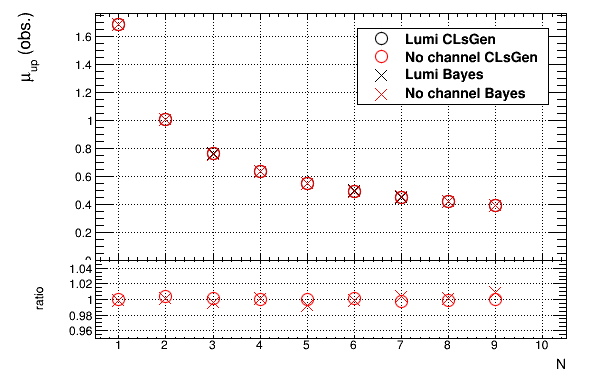
\includegraphics[scale=0.35]{figures/cLimitLumiVsNoChannels}
\end{figure}


\begin{center}

$\rightarrow$ Expectation verified in both CLsGenerator and BayesianMCMC

\end{center}


\lyxframeend{}\section{Uncertainties}


\lyxframeend{}\lyxframe{}

\begin{center}
\vspace*{2cm}
{\Large Uncertainties}
\end{center}


\lyxframeend{}\lyxframe{Problematic}
\begin{itemize}
\item Nominal signal and background yields ($s_{\text{nom}}$ and $b_{i}$)
not known with infinite precision
\item Two types of uncertainties

\begin{itemize}
\item statistical (finite sample size)
\item systematic (e.g. JES, JVF, etc.)\vspace{0.2cm}
\end{itemize}

\begin{center}


\textcolor{magenta}{$\rightarrow$ How to account for uncertainties
in limit setting ?}


\end{center}

\end{itemize}

\lyxframeend{}\lyxframe{Statistical uncertainties}
\begin{itemize}
\item Consider treatment of stat. uncert. as done in McLimit, CLsGenerator
and BayesianMCMC (HistFactory makes things differently)
\end{itemize}

\pause{\vspace*{0.2cm}}
\begin{itemize}
\item Signal and background are considered as random variables with

\begin{itemize}
\item average = nominal yields ($\sum w_{i}$)
\item standard deviation =$\left\{\begin{matrix} \text{stat. uncert. } (\sqrt{\sum w_i^2}) \text{ when nominal yield} \neq 0\\ \text{upper limit (1.14 lumi rescaled) when yield}=0  \end{matrix}\right.$ 
\end{itemize}
\end{itemize}
\vspace*{0.3cm}

\textbf{\textcolor{blue}{\small{Single channel}}}{\small \par}

\vspace*{-0.7cm}

\begin{center}

\textcolor{blue}{\small{$\boxed{{\color{black}{\cal \mathcal{L}}(\mu,s',\{b_{i}'\})=\frac{\left(\mu s'+\sum_{i}b_{i}'\right)^{N_{\text{obs}}}}{N_{\text{obs}}!}e^{-(\mu s'+\sum_{i}b_{i}')}\underbrace{f(s';s_{\text{nom}},\sigma_{s})}_{\text{constraint signal}}\prod\limits _{i}\underbrace{f(b_{i}';b_{i},\sigma_{i})}_{\text{constraint background i}}}}$}}{\small \par}

\end{center}


\pause{\vspace*{0.2cm}}
\begin{itemize}
\item \textcolor{magenta}{Terminology: $s'$ and $\{b_{i}'\}$ are called
nuisance parameters}
\end{itemize}

\lyxframeend{}\lyxframe{What McLimit/CLsGenerator/BayesianMCMC do ?}

\textbf{\textcolor{blue}{\small{Single channel}}}{\small \par}

\vspace*{-0.7cm}

\begin{center}

\textcolor{blue}{\small{$\boxed{{\color{black}{\cal \mathcal{L}}(\mu,s',\{b_{i}'\})=\frac{\left(\mu s'+\sum_{i}b_{i}'\right)^{N_{\text{obs}}}}{N_{\text{obs}}!}e^{-(\mu s'+\sum_{i}b_{i}')}\underbrace{f(s';s_{\text{nom}},\sigma_{s})}_{\text{constraint signal}}\prod\limits _{i}\underbrace{f(b_{i}';b_{i},\sigma_{i})}_{\text{constraint background i}}}}$}}{\small \par}

\end{center}


\pause{\vspace*{0.1cm}}
\begin{itemize}
\item McLimit/CLsGenerator toss pseudo-experiments in which

\begin{itemize}
\item $N_{\text{obs}}$ is sampled from marginal likelihood (hence the hybrid
nature of the method)


\begin{center}


\textrm{\textcolor{magenta}{\footnotesize{${\cal \mathcal{L}}(\mu)={\displaystyle \int}\frac{\left(\mu s'+\sum_{i}b_{i}'\right)^{N_{\text{obs}}}}{N_{\text{obs}}!}e^{-(\mu s'+\sum_{i}b_{i}')}f(s';s_{\text{nom}},\sigma_{s})\prod\limits _{i}f(b_{i}';b_{i},\sigma_{i})\text{d}s'\text{\ensuremath{\prod\limits _{i}}d}b_{i}'\quad(\square)$}}}{\footnotesize \par}


\end{center}

\item Test is computed using nominal values of nuisance parameters


\begin{center}


\textrm{\textcolor{magenta}{\footnotesize{${\cal \mathcal{L}}(\mu,s'=s_{nom},\{b_{i}'\}=b_{i})=\frac{\left(\mu s_{\text{nom}}+\sum_{i}b_{i}\right)^{N_{\text{obs}}}}{N_{\text{obs}}!}e^{-\left(\mu s_{\text{nom}}+\sum_{i}b_{i}\right)}$}}}{\footnotesize \par}


\end{center}

\end{itemize}
\end{itemize}

\pause{\vspace*{0.1cm}}
\begin{itemize}
\item BayesianMCMC uses marginal likelihood \textcolor{black}{\small{$(\square)$
}}as posterior (integration done by Markov Chain Monte Carlo)
\end{itemize}

\lyxframeend{}\lyxframe{Choice of constraint terms}
\begin{itemize}
\item This choice is to some extend arbitrary
\item However, care must be taken because some choices behave sometimes
badly
\item Common choices
\end{itemize}
\begin{table}
\begin{tabular}{|c|c|}
\hline 
Constraint p. d. f. & Available in\tabularnewline
\hline 
\hline 
Normal & McLimit, CLsGenerator, BayesianMCMC\tabularnewline
\hline 
Log-normal & CLsGenerator, BayesianMCMC\tabularnewline
\hline 
Gamma & CLsGenerator, BayesianMCMC\tabularnewline
\hline 
\end{tabular}

\end{table}



\lyxframeend{}\lyxframe{Comparison of distributions}

\begin{figure}
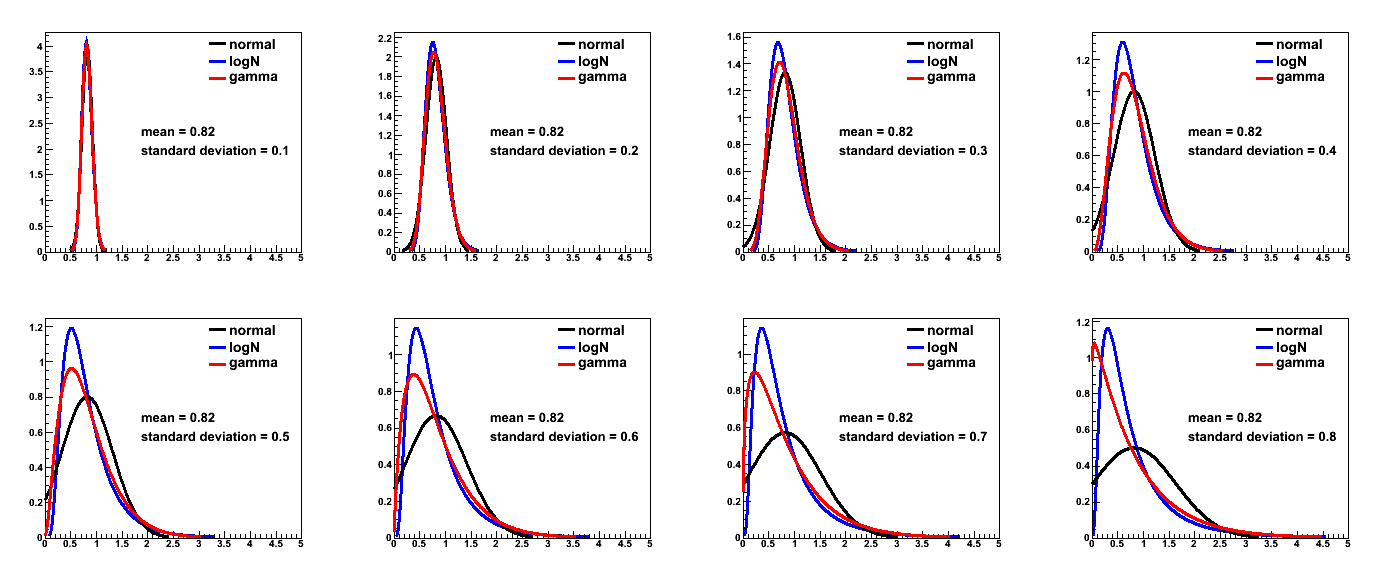
\includegraphics[scale=0.25]{figures/plotNormalLogNGamma}
\end{figure}



\lyxframeend{}\lyxframe{Effect of statistical uncertainty and constraint p. d. f.}
\begin{itemize}
\item $N_{obs}=1$, $b=0.82$ and $s=2.49$
\item Stat uncertainty on $b=0,...,1.4$
\end{itemize}
\begin{center}

\textcolor{black}{\tiny{CLsGenerator}}{\tiny \par}

\end{center}

\vspace*{-0.6cm}

\begin{figure}
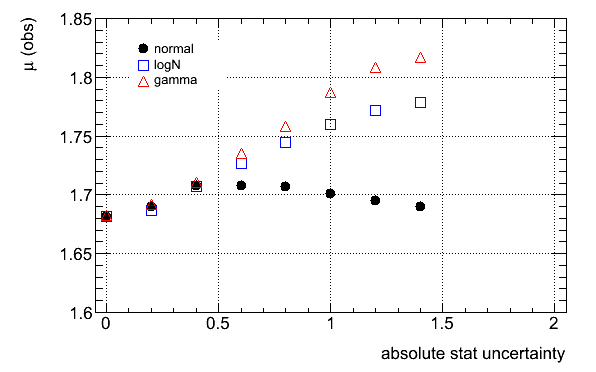
\includegraphics[scale=0.3]{figures/cLimit}
\end{figure}

\begin{itemize}
\item It can be shown that exactly the same results should be obtained with
BayesianMCMC when non stat. uncert. on signal

\begin{itemize}
\item It has been checked that it's actually the case
\end{itemize}
\end{itemize}

\lyxframeend{}\lyxframe{Effect of statistical uncertainty and constraint p. d. f.}

\begin{center}

\textcolor{black}{\scriptsize{normal (top), logN (middle) and gamma
(bottom)}}{\scriptsize \par}

\end{center}

\vspace*{-0.3cm}

\begin{figure}
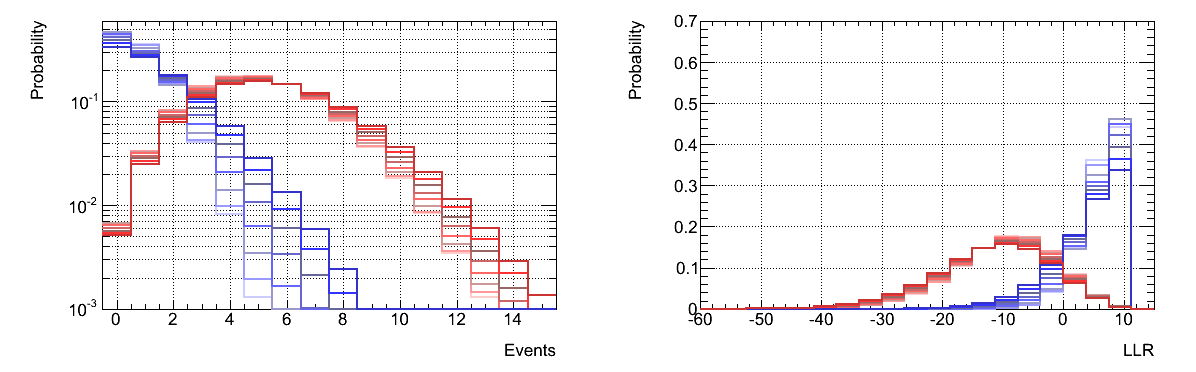
\includegraphics[scale=0.18]{figures/cDistrNormal}
\end{figure}
\vspace*{-0.4cm}

\begin{figure}
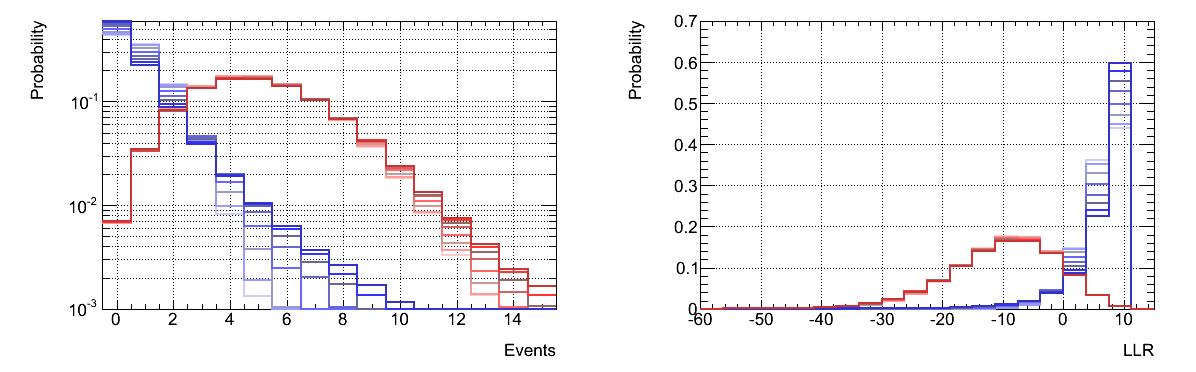
\includegraphics[scale=0.18]{figures/cDistrLogN}
\end{figure}
\vspace*{-0.4cm}

\begin{figure}
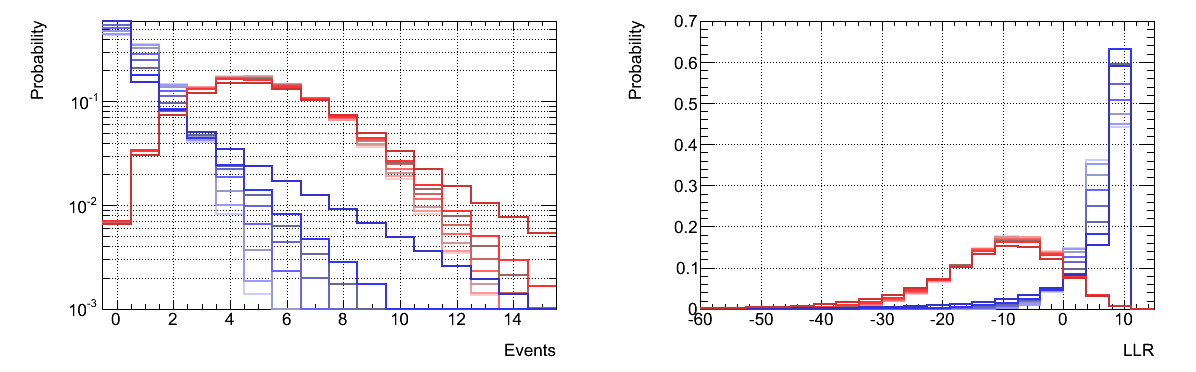
\includegraphics[scale=0.18]{figures/cDistrGamma}
\end{figure}



\lyxframeend{}\lyxframe{Effect of statistical uncertainty and constraint p. d. f.}
\begin{itemize}
\item Truncation at 0 in normal case doesn't smear distributions but shifts
them

\begin{itemize}
\item Happens for both b and s+b distribs $\Rightarrow\mu$ doesn't change
much 
\end{itemize}
\item logN smears less than gamma $\Rightarrow$ better $\mu$ for logN
than for gamma
\item What is the best choice ? logN ?
\end{itemize}
\begin{figure}
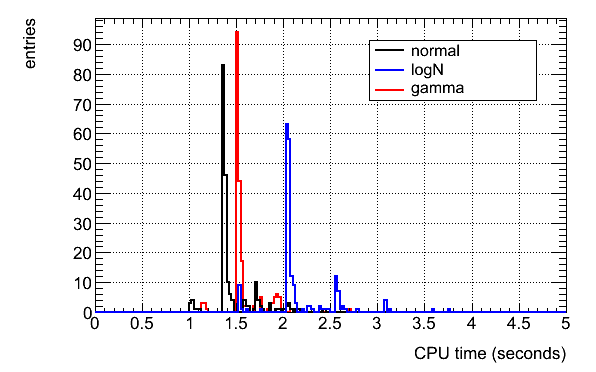
\includegraphics[scale=0.28]{figures/cCPUTime}
\end{figure}



\lyxframeend{}\lyxframe{Comparison of samplings for another particular case (1)}

\begin{minipage}[c]{0.3\columnwidth}%
\begin{itemize}
\item $N_{obs}=1$
\item $b=0.82$
\item $s=2.49$
\item No syst uncertainty
\item Stat uncertainty on $s$ and $b=0.1,...,1.4$\end{itemize}
%
\end{minipage}%
\begin{minipage}[c]{0.4\columnwidth}%
\begin{figure}
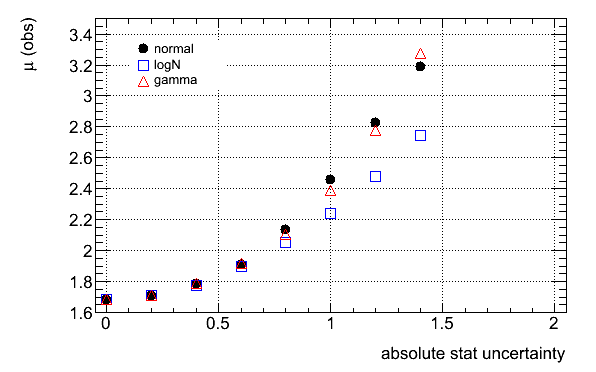
\includegraphics[scale=0.35]{figures/cLimit2}
\end{figure}
%
\end{minipage}


\lyxframeend{}\lyxframe{Comparison of samplings for another particular case (2)}

Normal (top), logN (middle) and Gamma (bottom)

\begin{figure}
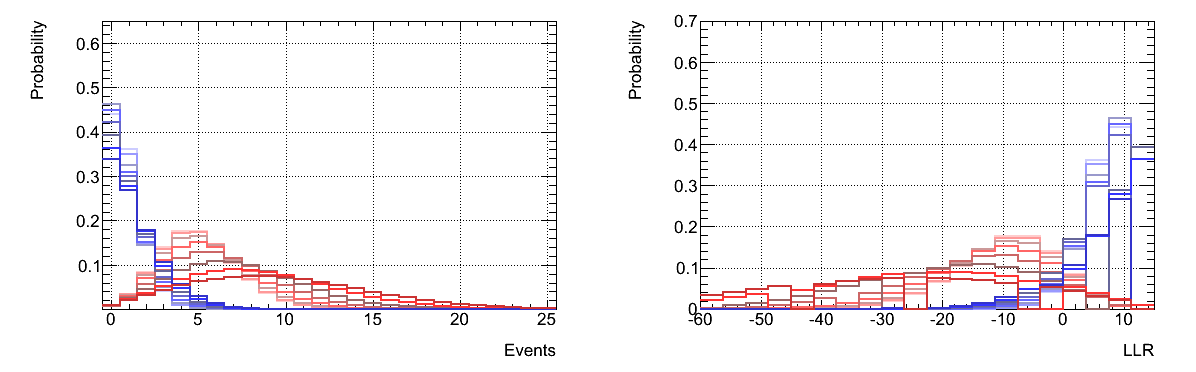
\includegraphics[scale=0.18]{figures/cDistrNormal2}
\end{figure}


\begin{figure}
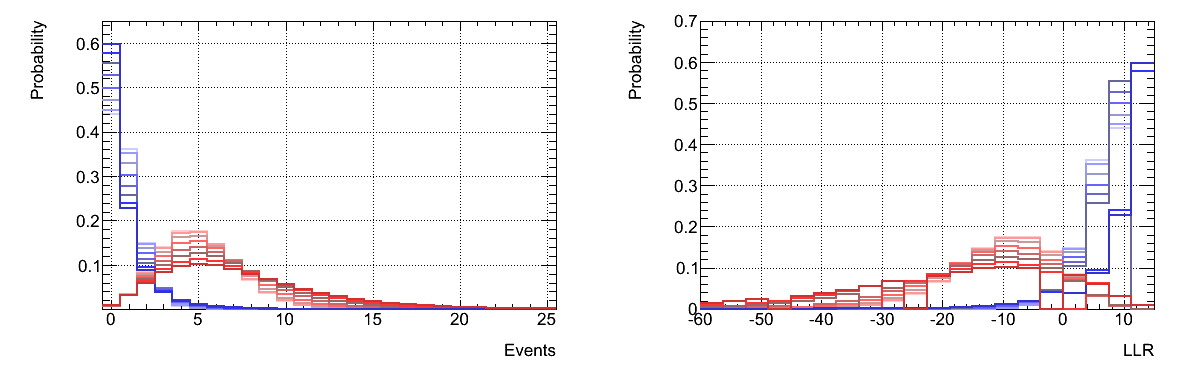
\includegraphics[scale=0.18]{figures/cDistrLogN2}
\end{figure}


\begin{figure}
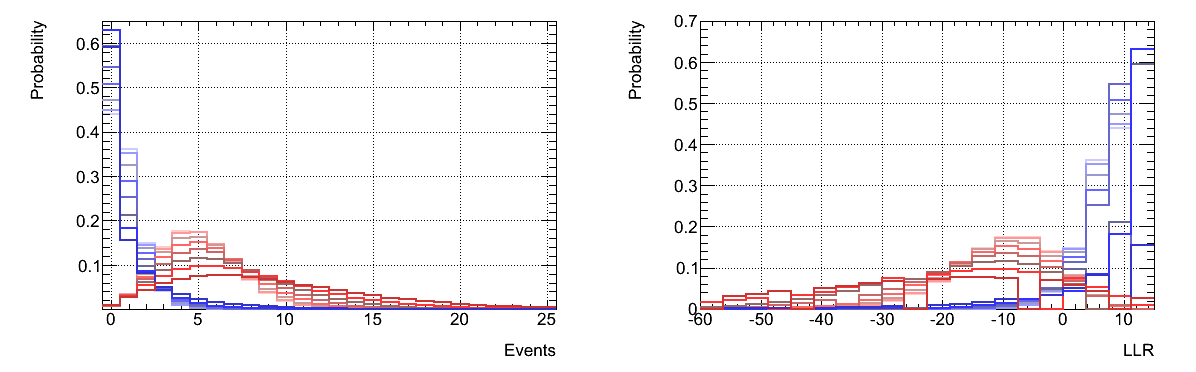
\includegraphics[scale=0.18]{figures/cDistrGamma2}
\end{figure}



\lyxframeend{}\lyxframe{Comparison of samplings for another particular case (3)}
\begin{itemize}
\item logN smears less than gamma $\Rightarrow$ better $\mu$ for logN
than for gamma (as in previous case)
\item Normal case now very different from previous case 

\begin{itemize}
\item s+b distribution is now ``more smeared'' than b alone distribution
$\Rightarrow$ have to go to larger $\mu$ to reach given confidence
level
\end{itemize}
\end{itemize}

\lyxframeend{}\lyxframe{}

\begin{center}
\vspace*{2cm}
{\Large Comparison of CLsGenerator and pure bayesian}
\end{center}


\lyxframeend{}\lyxframe{Purpose of the study}
\begin{itemize}
\item Purpose:

\begin{itemize}
\item Always interesting to compare various methods
\item Comparing the two approaches tells us how sensitive the analysis is
on the treatment of systematics

\begin{itemize}
\item $CL_{\text{s}}$ and bayesian with uniform prior are equivalent without
systematics $\Rightarrow$ differences arise only from the different
treatment of systematics
\end{itemize}
\end{itemize}
\item Bayesian implementation validated by comparing it to CLsGenerator/analytical
without systematics
\end{itemize}

\lyxframeend{}\lyxframe{Bayesian implementation}
\begin{itemize}
\item Statistical model built using RooFit/RooStat

\begin{itemize}
\item It is exactly the same as the CLsGenerator (mclimit) one
\item It is build from the same input files as CLsGenerator
\end{itemize}
\item Marginal likelihood is
\end{itemize}
\begin{center}

\textcolor{blue}{\scriptsize{${\color{blue}{\color{blue}}{\color{black}{\color{black}{\cal \mathcal{L}}_{\text{m}}(\mu)={\displaystyle \int}\frac{\left(\mu s+\sum_{i}b_{i}\right)^{N_{obs}}}{N_{obs}!}e^{-(\mu s+\sum_{i}b_{i})}\prod_{j}e^{-\frac{\eta_{j}^{2}}{2}}\prod_{i}e^{-\frac{(\gamma_{i}-1)^{2}}{2\sigma_{i}^{2}}}e^{-\frac{(\gamma_{s}-1)^{2}}{2\sigma_{s}^{2}}}\prod_{j}\text{d}\eta_{j}\prod_{i}\text{d}\gamma_{i}\text{d}\gamma_{s}}}}$}}{\scriptsize \par}

\end{center}
\begin{itemize}
\item Marginalization done by Markov Chain Monte Carlo
\end{itemize}

\lyxframeend{}\lyxframe{Visualization of Markov Chain}
\begin{itemize}
\item Plots below shows markov chain for following configuration:


\begin{tiny}


+bg Bkg 0.82 1


.syst Syst 0.02 -0.1


+sig Sig 2.49 0.4


+data 1


\end{tiny}

\end{itemize}
\vspace*{-0.5cm}

\begin{figure}
\centering{}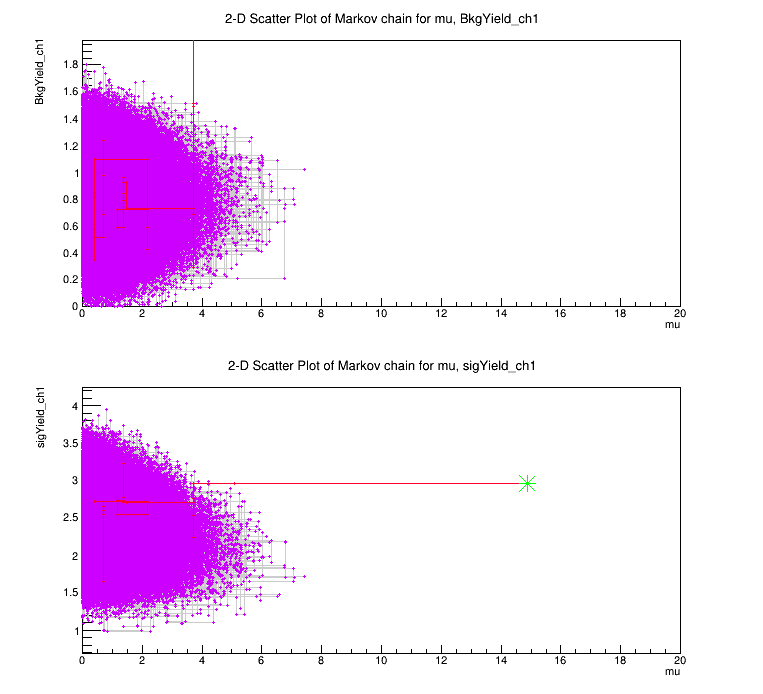
\includegraphics[scale=0.22]{figures/MarkovChainExample}
\end{figure}



\lyxframeend{}\lyxframe{Posterior}
\begin{itemize}
\item Plot below shows posterior and 95\% CL interval for same configuration
as in previous slide
\end{itemize}
\begin{figure}
\centering{}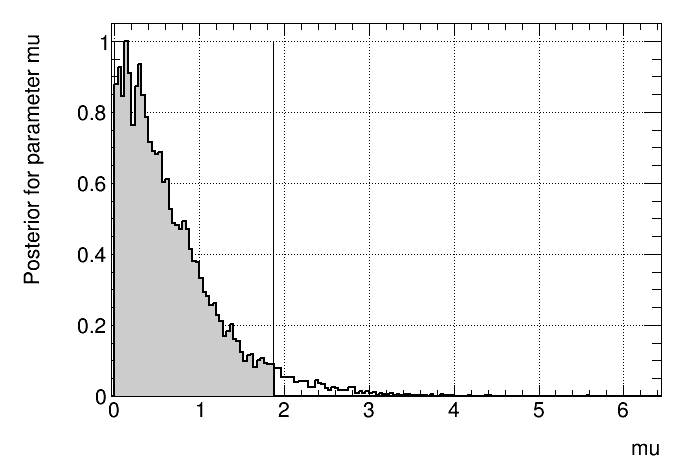
\includegraphics[scale=0.3]{figures/PosteriorExample}
\end{figure}



\lyxframeend{}\lyxframe{CLsGenerator/bayesian comparison with systematics}

\begin{minipage}[c]{0.4\columnwidth}%
\begin{itemize}
\item Configuration

\begin{itemize}
\item $N_{obs}=1$
\item $b=0.82$
\item $s=2.49$
\item Stat uncert. on $b$: $0.5$
\item Stat uncert. on $s$: $0.3$
\item Syst uncert. on $s$:

\begin{itemize}
\item up=$0.05$
\item down=$-0.05$
\end{itemize}
\item Syst uncert. on $b$ ($100\%$ correlated with $s$):

\begin{itemize}
\item up=$0.3$
\item down=$-0.3$\end{itemize}
\end{itemize}
\end{itemize}
%
\end{minipage}%
\begin{minipage}[c]{0.4\columnwidth}%
\begin{figure}
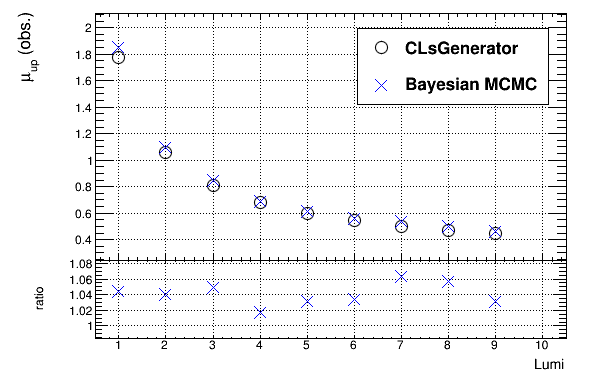
\includegraphics[scale=0.35]{figures/cLimitCLsGenVsBayesianWithSystCase1}
\end{figure}
%
\end{minipage}
\begin{itemize}
\item Effect of systematics treatment difference starts to be visible
\item Need to study the effect of systematics further in both cases
\end{itemize}

\lyxframeend{}\lyxframe{}

\begin{center}
\vspace*{2cm}
{\Large Studies on interpolation/extrapolation in CLsGenerator}
\end{center}


\lyxframeend{}\lyxframe{Interpolation/extrapolation of systematics (1)}
\begin{itemize}
\item For one sample and one systematic uncertainty we know 

\begin{itemize}
\item $N_{nom}$: nominal yield
\item $N_{\uparrow}$: yield with systematic varied $1\sigma$ up
\item $N_{\downarrow}$: yield with systematic varied $1\sigma$ dow
\end{itemize}

\pause{}

\item However, for the purpose of setting limits we need a continuous parametrization
of the yield: $N(\eta)$

\begin{itemize}
\item $\eta$ defined such that $N(\eta=0)=N_{nom}$, $N(\eta=+1)=N_{\uparrow}$
and $N(\eta=-1)=N_{\downarrow}$
\end{itemize}

\pause{}

\item \textcolor{red}{How do we interpolate for $\eta=[-1,1]$ and extrapolate
for $\eta<-1$ and $\eta>$1 ?}
\end{itemize}

\lyxframeend{}\lyxframe{Interpolation/extrapolation of systematics (2)}

Example : $N_{nom}=15,$ $N_{\uparrow}=21$, $N_{\downarrow}=10.5$

\begin{figure}
\begin{centering}
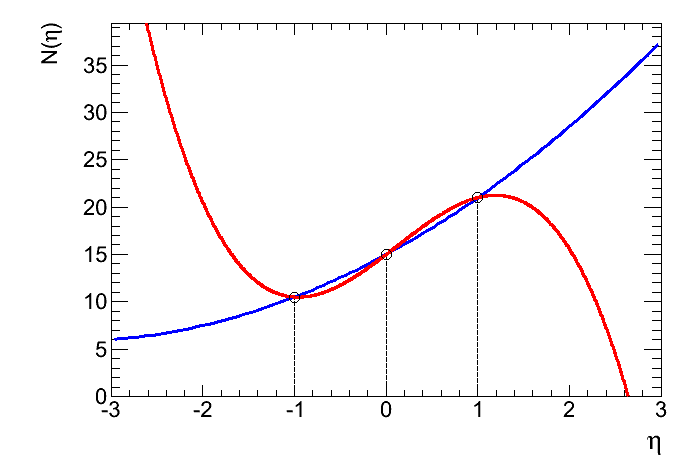
\includegraphics[scale=0.4]{figures/InterExtrapPrinciple}
\par\end{centering}

\end{figure}



\lyxframeend{}\lyxframe{Interpolation/extrapolation of systematics (3)}
\begin{itemize}
\item Rather than using $N_{nom,\uparrow,\downarrow}$, let's use

\begin{itemize}
\item $f^{\uparrow}=\frac{N_{\uparrow}-N_{nom}}{N_{nom}}$
\item $f^{\downarrow}=\frac{N_{\downarrow}-N_{nom}}{N_{nom}}$
\item $f^{syst}(\eta)=\frac{N(\eta)}{N_{nom}}$
\end{itemize}

\pause{}

\item One has 

\begin{itemize}
\item $f^{syst}(\eta=0)$ = 1
\item $f^{syst}(\eta=-1)=1+f^{\downarrow}$
\item $f^{syst}(\eta=1)=1+f^{\uparrow}$
\end{itemize}

\pause{}

\item \textcolor{red}{Goal: find an inter/extrapolation algorithm such that
these relations are satisfied (at least approximately) }
\end{itemize}

\lyxframeend{}\lyxframe{First look at mclimit, linear and exponential algorithms}

\begin{figure}


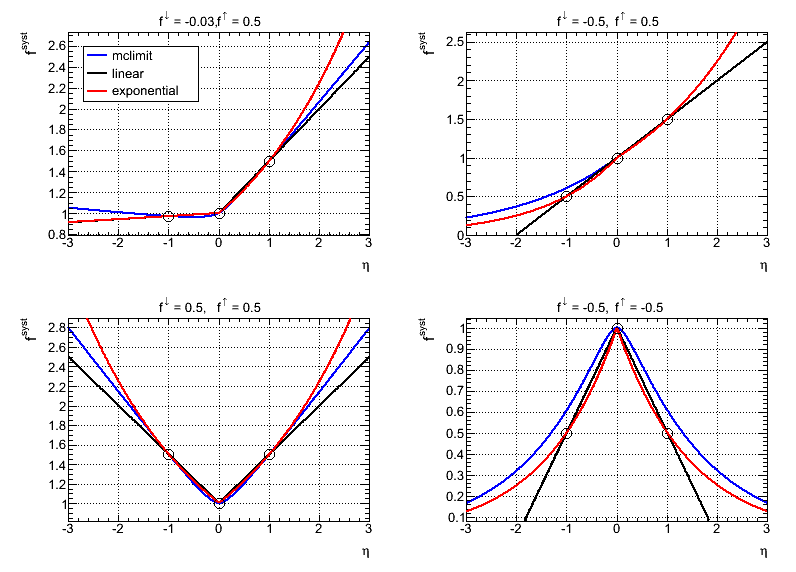
\includegraphics[scale=0.5]{figures/FewExamplesOffsyst}
\end{figure}



\lyxframeend{}\lyxframe{Closer look at mclimit algorithm (1)}
\begin{itemize}
\item What does mclimit give for $\eta=-1,0,+1$ ?

\begin{itemize}
\item $f^{syst}(\eta=0)=1$
\item if $f^{\uparrow}\geq0$: $f^{syst}(\eta=+1)=1+f^{\uparrow}$
\item if $f^{\downarrow}\geq0$: $f^{syst}(\eta=-1)=1+f^{\downarrow}$ 
\item if $f^{\uparrow}<0$: $f^{syst}(\eta=+1)=e^{f^{\uparrow}}$
\item if $f^{\downarrow}<0$: $f^{syst}(\eta=-1)=e^{f^{\downarrow}}$
\end{itemize}

\textcolor{blue}{In the last two cases, $f^{syst}\simeq1+f^{\uparrow(\downarrow)}$
only if }\textrm{\textcolor{blue}{$f^{\uparrow(\downarrow)}\simeq0$
(if $f^{\uparrow(\downarrow)}\simeq-1$, difference can be large).}}

\end{itemize}

\lyxframeend{}\lyxframe{Closer look at mclimit algorithm (2)}
\begin{itemize}
\item What does mclimit give when uncertainties are symetric: $f^{\uparrow}=-f^{\downarrow}$
?

\begin{itemize}
\item $\eta>0$: 

\begin{itemize}
\item $f^{\uparrow}\geq0$: $f^{syst}=1+\eta f^{\uparrow}$
\item $f^{\uparrow}<0$: $f^{syst}=e^{\eta f^{\uparrow}}$
\end{itemize}
\item $\eta<0$: 

\begin{itemize}
\item $f^{\downarrow}\ge0$: $f^{syst}=1-\eta f^{\downarrow}$
\item $f^{\downarrow}<0$: $f^{syst}=e^{-\eta f^{\downarrow}}$
\end{itemize}
\end{itemize}

\textcolor{blue}{mclimit is equivalent to linear for $\eta>0$ if
$f^{\uparrow}\geq0$ or $\eta<0$ if $f^{\downarrow}\geq\text{0}$}

\end{itemize}

\lyxframeend{}\lyxframe{Comparison of algorithms: test 1}

\begin{minipage}[c]{0.5\columnwidth}%
\begin{itemize}
\item $N_{obs}=1$
\item $b=0.82$
\item $s=2.49$
\item No stat uncertainty
\item No syst uncertainty on $s$
\item Syst uncertainty on $b$: $f^{\uparrow}=-f^{\downarrow}=0,0.1,0.2,\hdots,0.9$\end{itemize}
%
\end{minipage}%
\begin{minipage}[c]{0.4\columnwidth}%
\begin{figure}
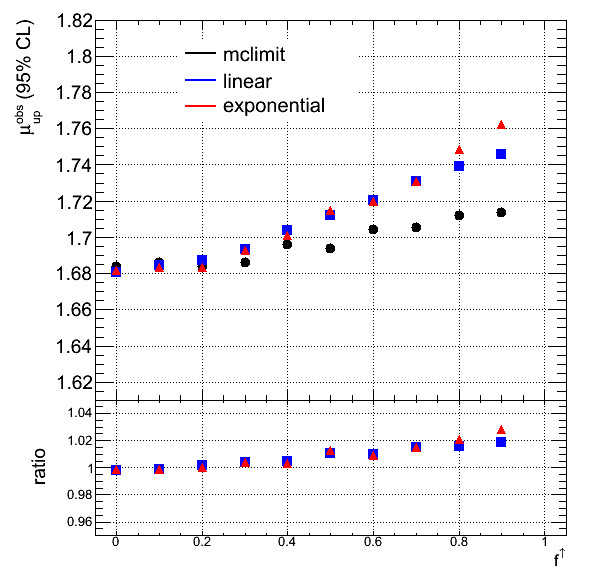
\includegraphics[scale=0.3]{figures/muUpVsSyst_case1}

\end{figure}
%
\end{minipage}


\lyxframeend{}\lyxframe{Comparison of algorithms: test 2}

\begin{minipage}[c]{0.5\columnwidth}%
\begin{itemize}
\item $N_{obs}=100$
\item $b=100$
\item $s=20$
\item No stat uncertainty
\item No syst uncertainty on $s$
\item Syst uncertainty on $b$: $f^{\uparrow}=-f^{\downarrow}=0,0.1,0.2,\hdots,0.9$\end{itemize}
%
\end{minipage}%
\begin{minipage}[c]{0.4\columnwidth}%
\begin{figure}
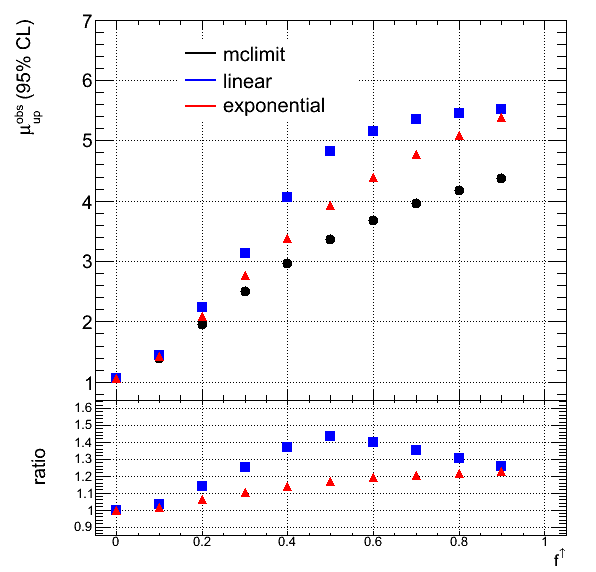
\includegraphics[scale=0.3]{figures/muUpVsSyst_case2}
\end{figure}
%
\end{minipage}


\lyxframeend{}\lyxframe{Comparison of algorithms: test 3}

\begin{minipage}[t]{1\columnwidth}%
\begin{minipage}[c]{0.45\columnwidth}%
\begin{itemize}
\item $N_{obs}=1$
\item $b=0.82$
\item $s=2.49$
\item No stat uncertainty
\item Syst uncertainty on $s$ and $b$ (100\% correlated): $f^{\uparrow}=-f^{\downarrow}=0,0.1,0.2,\hdots,0.6$\end{itemize}
%
\end{minipage}%
\begin{minipage}[c]{0.45\columnwidth}%
\begin{figure}
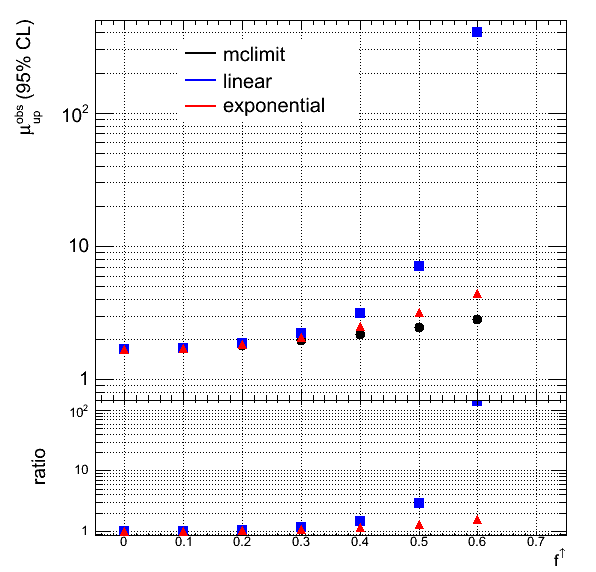
\includegraphics[scale=0.25]{figures/muUpVsSyst_case3}
\end{figure}
%
\end{minipage}

Comments: 
\begin{itemize}
\item $q_{\mu}=2\left(\mu s-N_{obs}\ln\frac{\mu s+b}{b}\right)$
\item When \textrm{$f^{\downarrow}\ll0$, $f^{syst}=0$ quite frequently}
$\Rightarrow s=b=0\Rightarrow N_{obs}=0\Rightarrow q_{\mu}=2\mu s\text{ (for both hypothesis)\ensuremath{\Rightarrow}}$CL$_{s+b}$
and CL$_{s}$ can't go to very low values as $\mu$ increases\end{itemize}
%
\end{minipage}


\lyxframeend{}\lyxframe{Comparison of algorithms: test 3 (cont'd)}

Consider the point $f^{\uparrow}=-f^{\downarrow}=0.6$

\begin{minipage}[c]{1\columnwidth}%
\begin{minipage}[c]{0.32\columnwidth}%
\begin{figure}
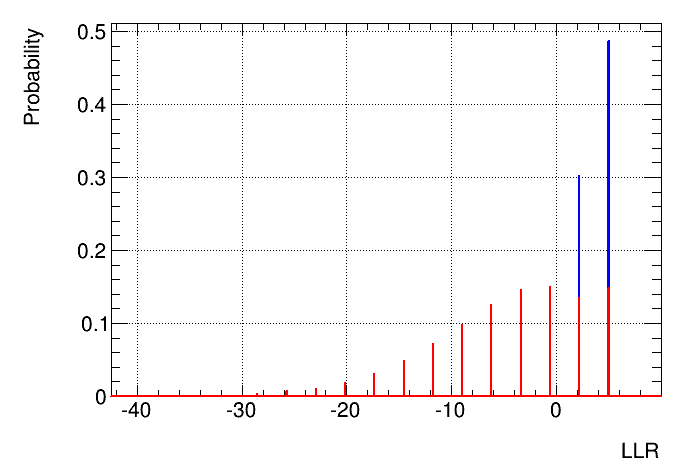
\includegraphics[scale=0.15]{figures/LLR_syst6_mu1}

\textcolor{black}{\scriptsize{${\mu=1}$}}
\end{figure}
%
\end{minipage}%
\begin{minipage}[c]{0.32\columnwidth}%
\begin{figure}


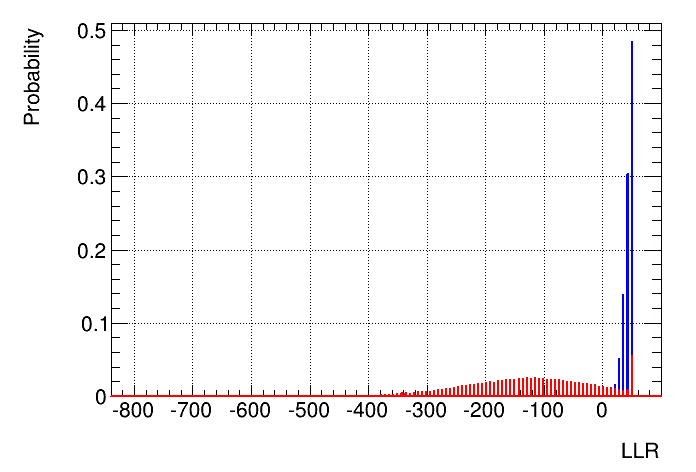
\includegraphics[scale=0.15]{figures/LLR_syst6_mu10}

\textcolor{black}{\scriptsize{$\mu=10$}}
\end{figure}
%
\end{minipage}%
\begin{minipage}[c]{0.32\columnwidth}%
\begin{figure}


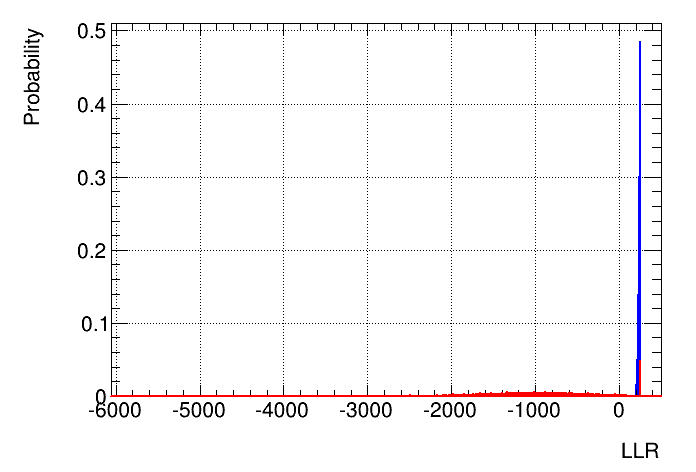
\includegraphics[scale=0.15]{figures/LLR_syst6_mu50}

\textcolor{black}{\scriptsize{$\mu=50$}}
\end{figure}
%
\end{minipage}%
\end{minipage}

\begin{figure}
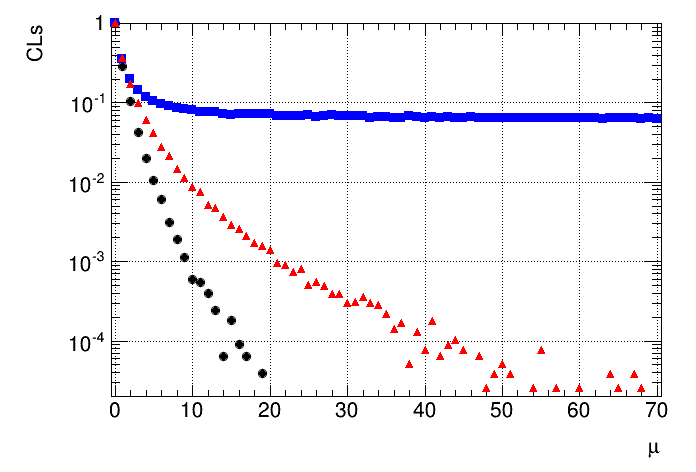
\includegraphics[scale=0.3]{figures/CLsVsMu_case3_SystEq6}
\end{figure}



\lyxframeend{}\lyxframe{Comparison of algorithms: test 3 (cont'd)}
\begin{itemize}
\item After having studied a few situations by varying systematics on signal,
backgrounds and correlations, it appears that one should be very careful
with linear inter/extrapolation

\begin{itemize}
\item when signal systematic uncertainty is large

\begin{itemize}
\item when in addition background systematics are large effect is more pronounced
\item when in addition background systematics are large and correlated to
signal systematics effect can be dramatic (see two previous slides)
\end{itemize}
\end{itemize}
\item Remark: effect exists only if $f^{\uparrow}$ and/or $f^{\downarrow}$
(for the signal at least) is negative
\end{itemize}

\lyxframeend{}\lyxframe{Comparison of algorithms: LHCP mumu channel}

Here we use 4tmm.dat from David (with +data 1)
\begin{itemize}
\item Limits
\begin{table}


\begin{tabular}{|c|c|c|c|}
\hline 
 & mclimit & linear & expo\tabularnewline
\hline 
\hline 
Expected median & 1.70 & 1.70 & 1.69\tabularnewline
\hline 
Expected $\pm1\sigma$ & 1.44-2.08 & 1.43-2.07 & 1.43-2.07\tabularnewline
\hline 
Expected $\pm2\sigma$ & 1.26-3.52 & 1.27-3.53 & 1.27-3.54\tabularnewline
\hline 
Observed & 1.67 & 1.68 & 1.67\tabularnewline
\hline 
\end{tabular}
\end{table}
Conclusion: the three algorithms give compatible results
\end{itemize}
\begin{minipage}[t]{1\columnwidth}%
\begin{minipage}[t]{0.4\columnwidth}%
\begin{itemize}
\item CPU time 


\textcolor{black}{\scriptsize{ran}} \textcolor{black}{\scriptsize{clgen.observedSigStrengthFor95excl(0,1e5,cls)
in identical conditions several times to make this distrib}}\end{itemize}
%
\end{minipage}%
\begin{minipage}[t]{0.75\columnwidth}%
\begin{figure}
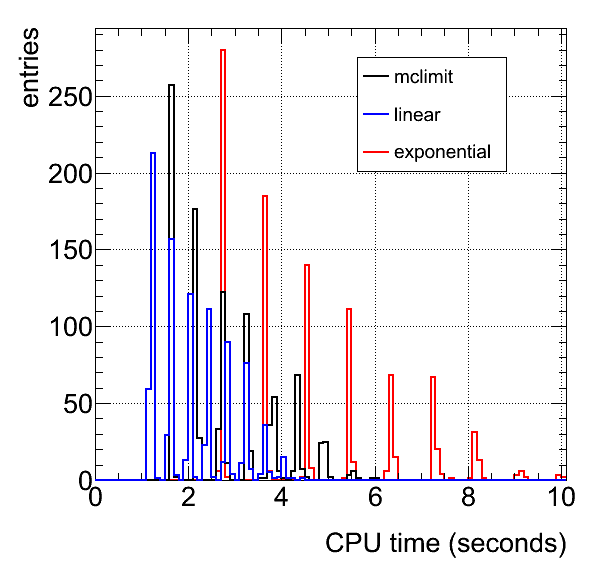
\includegraphics[scale=0.2]{figures/CPUtime}
\end{figure}
%
\end{minipage}%
\end{minipage}


\lyxframeend{}\lyxframe{Understanding $f^{syst}$ distribution: exponential case}
\begin{itemize}
\item $f^{syst}$ sometimes looks very weird. Let's consider exponential
algo with $f^{\downarrow}=-0.1$ and $f^{\uparrow}=0.6$ (on the plot,
Variation=$f^{syst}$)
\end{itemize}
\vspace*{-0.2cm}

\begin{figure}
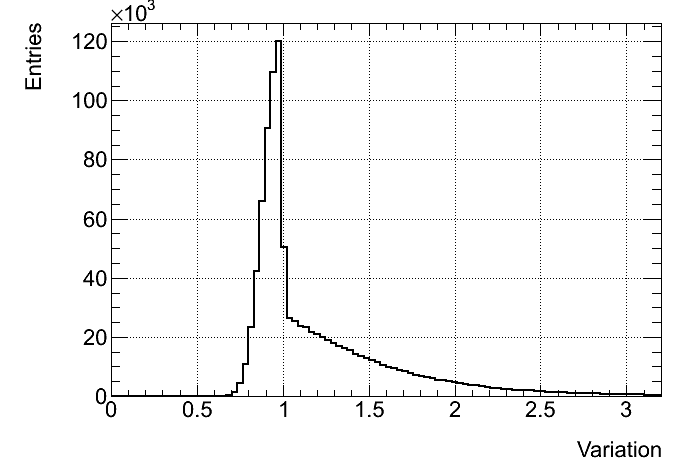
\includegraphics[scale=0.2]{figures/fsystDistr_minus01_plus06_expo}
\end{figure}


\vspace*{-0.5cm}
\begin{itemize}
\item Where does this funny looking shape comes from ?

\begin{itemize}
\item We have $f^{syst}=(1+f^{\uparrow})^{\eta}$ for $\eta>0$ ($(1+f^{\uparrow})^{-\eta}$
for $\eta<0$ ) with $\eta\sim\mathcal{N}(0,1)$
\item It's straightforward to show that \textcolor{black}{\scriptsize{$f^{syst}\sim\frac{1}{\sqrt{2\pi}|\ln\left(1+f^{\uparrow(\downarrow)}\right)|f^{syst}}e^{-\frac{1}{2}\left(\frac{\ln f^{syst}}{\ln\left(1+f^{\uparrow(\downarrow)}\right)}\right)^{2}}$ }}{\scriptsize \par}
\item i.e. $f^{syst}\sim\text{piecewise }log\mathcal{N}$
\end{itemize}
\item Note: understanding the shape of a distribution doesn't mean that
such a distribution is desirable $\rightarrow$ is it ?
\end{itemize}

\lyxframeend{}\lyxframe{Understanding $f^{syst}$ distribution: linear and mclimit cases}
\begin{itemize}
\item linear case is obvious: $f^{syst}\sim$ piecewise gaussian truncated
at 0. Using values of previous slide we have
\end{itemize}
\vspace*{-0.2cm}

\begin{figure}
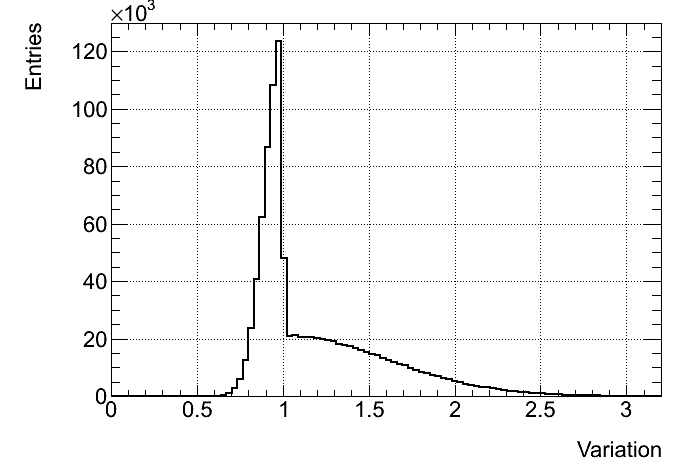
\includegraphics[scale=0.2]{figures/fsystDistr_minus01_plus06_linear}
\end{figure}


\vspace*{-0.5cm}
\begin{itemize}
\item mclimit case: doesn't seem to be possible to determine analytic solution.
Using values of previous slide we have
\end{itemize}
\vspace*{-0.2cm}

\begin{figure}
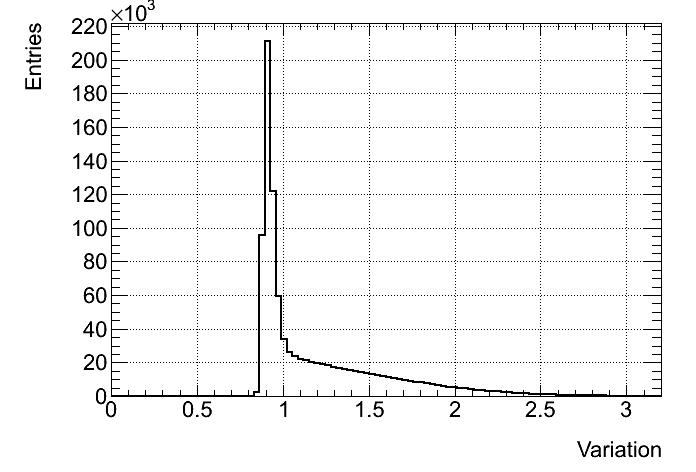
\includegraphics[scale=0.2]{figures/fsystDistr_minus01_plus06_mclimit}
\end{figure}


\vspace*{-0.5cm}


\lyxframeend{}\lyxframe{Coming back to test 2}
\begin{itemize}
\item In some extreme cases (very large systematics), linear and expo give
really really worrying distributions
\item Let's consider the point $f^{\uparrow}=-f^{\downarrow}=0.9$ and $\mu=5.5$
of test 2.
\end{itemize}
\begin{minipage}[c]{1\columnwidth}%
\begin{minipage}[c]{0.32\columnwidth}%
\begin{figure}
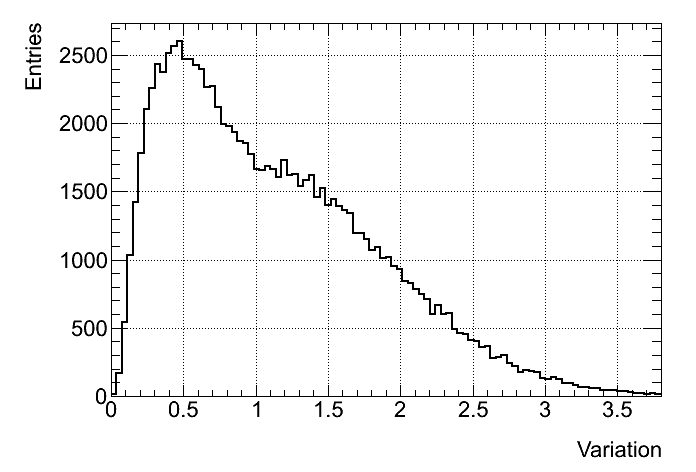
\includegraphics[scale=0.15]{figures/fsyst_mclimit_test2_9_9}
\end{figure}
%
\end{minipage}%
\begin{minipage}[c]{0.32\columnwidth}%
\begin{figure}
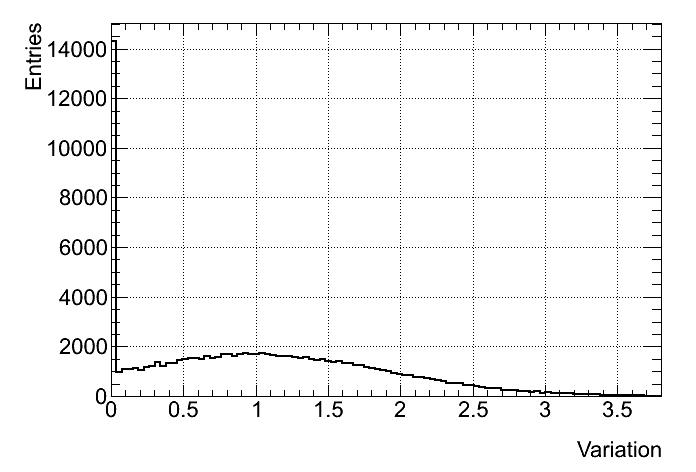
\includegraphics[scale=0.15]{figures/fsyst_linear_test2_9_9}
\end{figure}
%
\end{minipage}%
\begin{minipage}[c]{0.32\columnwidth}%
\begin{figure}
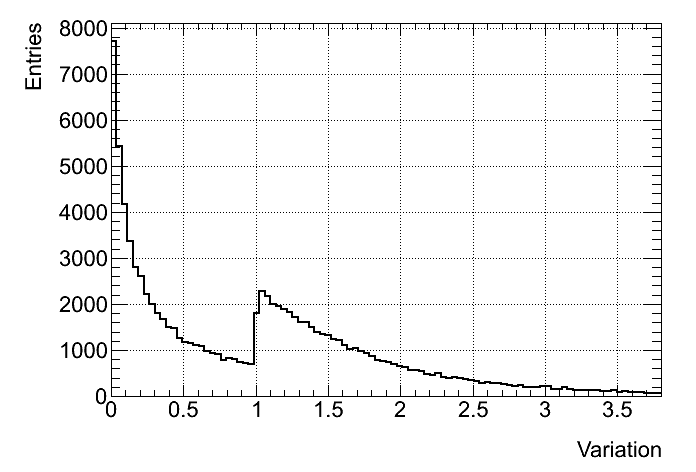
\includegraphics[scale=0.15]{figures/fsyst_expo_test2_9_9}
\end{figure}
%
\end{minipage}%
\end{minipage}

\begin{minipage}[c]{1\columnwidth}%
\begin{minipage}[c]{0.32\columnwidth}%
\begin{figure}
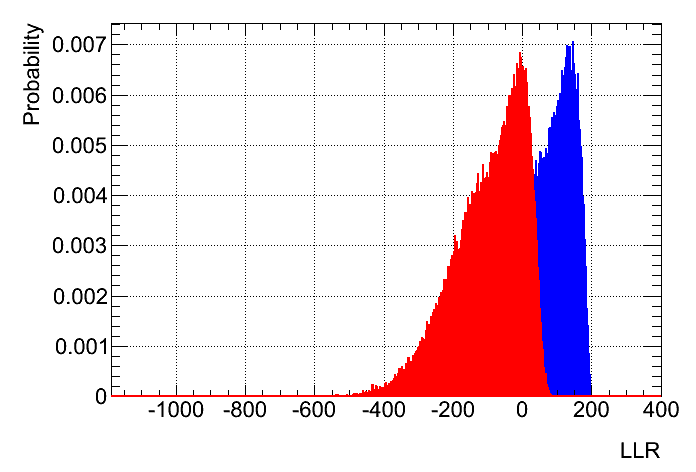
\includegraphics[scale=0.15]{figures/LLR_mclimit_test2_9_9}

\textcolor{black}{\tiny{mclimit}}
\end{figure}
%
\end{minipage}%
\begin{minipage}[c]{0.32\columnwidth}%
\begin{figure}
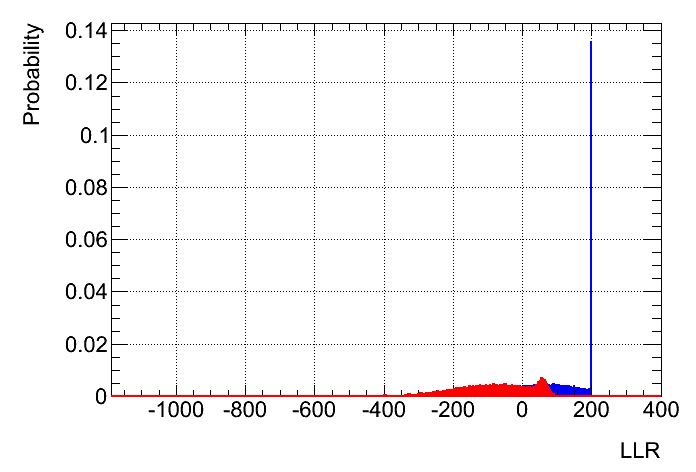
\includegraphics[scale=0.15]{figures/LLR_linear_test2_9_9}

\textcolor{black}{\tiny{linear}}
\end{figure}
%
\end{minipage}%
\begin{minipage}[c]{0.32\columnwidth}%
\begin{figure}
\includegraphics[scale=0.15]{figures/LLR_expo_test2_9_9}

\textcolor{black}{\tiny{expo}}
\end{figure}
%
\end{minipage}%
\end{minipage}
\begin{itemize}
\item Using truncated piecewise gaussian (linear) and piecewise $log\text{\ensuremath{\mathcal{N}}}$
(expo) seems to be absurd $\rightarrow$mclimit seems to be much more
reasonable in such large systematics case
\end{itemize}

\lyxframeend{}\lyxframe{Preliminary conclusions (1)}
\begin{itemize}
\item mclimit, linear and exponential algorithms give similar results for
small systematics

\begin{itemize}
\item Any choice seems to be rather safe in this case
\end{itemize}
\item Differences can be significant for large systematics

\begin{itemize}
\item linear shouldn't be used when signal systematics (and background ?)
are large
\item expo shouldn't be used when systematics on background and/or signal
are large and $f^{\downarrow}\text{\text{or}}f^{\uparrow}\ll0$
\item mclimit seems to be the safest choice when systematics are large
\end{itemize}
\item Argument of continuous derivative which at first sight seemed important
only for MINUIT is actually also important when no fitting is done
as it provides distributions of $f^{syst}$ that are smooth (particularly
important for large systematics).
\end{itemize}

\lyxframeend{}\lyxframe{Preliminary conclusions (2)}
\begin{itemize}
\item mclimit:

\begin{itemize}
\item pros: $f^{syst}$ smooth, $f^{syst}(\eta)\text{\ensuremath{\neq}0 \ensuremath{\forall\eta}}$
\item cons: $f^{syst}(\eta=\pm1)\neq1+f^{\uparrow(\downarrow)}$ when $f^{\uparrow(\downarrow)}<0$, 
\end{itemize}
\item linear:

\begin{itemize}
\item pros: simple, fast
\item cons: $f^{syst}(\eta)\text{=0}$ in some cases ($\Rightarrow$ problem
when signal syst large)
\end{itemize}
\item expo: 

\begin{itemize}
\item pros: simple, $f^{syst}(\eta)\text{\ensuremath{\neq}0 \ensuremath{\forall\eta}}$
\item cons: $f^{syst}$ can be very discontinuous for large $f^{\uparrow(\downarrow)}$,
slow
\end{itemize}
\end{itemize}

\lyxframeend{}\lyxframe{Preliminary conclusions (3)}
\begin{itemize}
\item Systematics are such a pain ! It's good that we're not affected too
much by them in the same-sign analysis
\end{itemize}

\lyxframeend{}\lyxframe{Ideas for further studies (1)}
\begin{itemize}
\item Try linear interpolation and expo extrapolation
\item Alternative to TMath::Power() for exponential case ?
\item Try $\eta\sim log\mathcal{\mathcal{N}}$

\begin{itemize}
\item Note that $\eta\sim log\mathcal{N}$ + linear is equivalent to $\eta\sim\mathcal{N}$+
expo (in both cases $f^{syst}\sim log\mathcal{N}$)

\begin{itemize}
\item As $\eta\sim\mathcal{N}$+ expo is quite slow, could be interesting
to see if it's faster in terms of CPU to do $\eta\sim log\mathcal{N}$
+ linear
\end{itemize}
\end{itemize}
\item Try $\eta\sim Gamma$
\end{itemize}

\lyxframeend{}\lyxframe{Ideas for further studies (2)}
\begin{block}
<1->{Statistical model}

${\cal \mathcal{L}}(\mu,\{\eta\},\{\gamma\})=\frac{\left(\mu s+\sum_{i}b_{i}\right)^{N_{obs}}}{N_{obs}!}e^{-(\mu s+\sum_{i}b_{i})}$


where 
\begin{itemize}
\item $b_{i}=b_{i}(\{\eta\},\{\gamma\})=b_{i}^{nom}\times\prod_{j}f_{ij}(\eta_{j})\times\gamma_{i}$ 
\item $s=s(\{\eta\},\{\gamma\})=s^{nom}\times\prod_{j}f_{j}^{s}(\eta_{j})\times\gamma_{s}$ 
\end{itemize}

and
\begin{itemize}
\item $\eta_{j}\sim\mathcal{N}(0,1)$
\item $\gamma_{i}\sim\mathcal{N}(1,\sigma_{i})$ and \textrm{$\gamma_{s}\sim\mathcal{N}(1,\sigma_{s})$}
\end{itemize}
\end{block}
\begin{itemize}
\item When generating pseudo exp, $N_{obs}$ generated according to marginal
likelihood:


\textcolor{blue}{\scriptsize{${\color{blue}{\color{blue}}{\color{black}{\color{black}{\cal \mathcal{L}}_{\text{m}}(\mu)={\displaystyle \int}\frac{\left(\mu s+\sum_{i}b_{i}\right)^{N_{obs}}}{N_{obs}!}e^{-(\mu s+\sum_{i}b_{i})}\prod_{j}e^{-\frac{\eta_{j}^{2}}{2}}\prod_{i}e^{-\frac{(\gamma_{i}-1)^{2}}{2\sigma_{i}^{2}}}e^{-\frac{(\gamma_{s}-1)^{2}}{2\sigma_{s}^{2}}}\prod_{j}\text{d}\eta_{j}\prod_{i}\text{d}\gamma_{i}\text{d}\gamma_{s}}}}$}}{\scriptsize \par}


However, ${\cal \mathcal{L}}(\mu,\{\eta\}=0,\{\gamma\}=1)$ is used
to calculate the test 


$\Rightarrow$ try calculating the test with marginal likelihood

\end{itemize}

\lyxframeend{}\lyxframe{Vrac}
\begin{itemize}
\item Popper
\item Construction Neyman
\end{itemize}

\lyxframeend{}
\end{document}
